% Options for packages loaded elsewhere
\PassOptionsToPackage{unicode}{hyperref}
\PassOptionsToPackage{hyphens}{url}
%
\documentclass[
]{book}
\usepackage{amsmath,amssymb}
\usepackage{iftex}
\ifPDFTeX
  \usepackage[T1]{fontenc}
  \usepackage[utf8]{inputenc}
  \usepackage{textcomp} % provide euro and other symbols
\else % if luatex or xetex
  \usepackage{unicode-math} % this also loads fontspec
  \defaultfontfeatures{Scale=MatchLowercase}
  \defaultfontfeatures[\rmfamily]{Ligatures=TeX,Scale=1}
\fi
\usepackage{lmodern}
\ifPDFTeX\else
  % xetex/luatex font selection
\fi
% Use upquote if available, for straight quotes in verbatim environments
\IfFileExists{upquote.sty}{\usepackage{upquote}}{}
\IfFileExists{microtype.sty}{% use microtype if available
  \usepackage[]{microtype}
  \UseMicrotypeSet[protrusion]{basicmath} % disable protrusion for tt fonts
}{}
\makeatletter
\@ifundefined{KOMAClassName}{% if non-KOMA class
  \IfFileExists{parskip.sty}{%
    \usepackage{parskip}
  }{% else
    \setlength{\parindent}{0pt}
    \setlength{\parskip}{6pt plus 2pt minus 1pt}}
}{% if KOMA class
  \KOMAoptions{parskip=half}}
\makeatother
\usepackage{xcolor}
\usepackage{longtable,booktabs,array}
\usepackage{calc} % for calculating minipage widths
% Correct order of tables after \paragraph or \subparagraph
\usepackage{etoolbox}
\makeatletter
\patchcmd\longtable{\par}{\if@noskipsec\mbox{}\fi\par}{}{}
\makeatother
% Allow footnotes in longtable head/foot
\IfFileExists{footnotehyper.sty}{\usepackage{footnotehyper}}{\usepackage{footnote}}
\makesavenoteenv{longtable}
\usepackage{graphicx}
\makeatletter
\def\maxwidth{\ifdim\Gin@nat@width>\linewidth\linewidth\else\Gin@nat@width\fi}
\def\maxheight{\ifdim\Gin@nat@height>\textheight\textheight\else\Gin@nat@height\fi}
\makeatother
% Scale images if necessary, so that they will not overflow the page
% margins by default, and it is still possible to overwrite the defaults
% using explicit options in \includegraphics[width, height, ...]{}
\setkeys{Gin}{width=\maxwidth,height=\maxheight,keepaspectratio}
% Set default figure placement to htbp
\makeatletter
\def\fps@figure{htbp}
\makeatother
\setlength{\emergencystretch}{3em} % prevent overfull lines
\providecommand{\tightlist}{%
  \setlength{\itemsep}{0pt}\setlength{\parskip}{0pt}}
\setcounter{secnumdepth}{5}
\usepackage{fontspec}
\usepackage{xltxtra}
\XeTeXlinebreaklocale "th_TH"
\XeTeXlinebreakskip = 0pt plus 1pt  
\usepackage{fonts-tlwg}

\setmainfont[Script=Thai,%
    Scale=MatchLowercase,%
    WordSpace=1.25,%
    Mapping=tex-text,]{TH Sarabun New}

%% ---- Load line spacing package ---- %%
\usepackage{setspace}

% Introducing hair space 
\newrobustcmd{\hrsp}{\ifmmode\mskip1mu\else\kern0.0625em\fi}





\usepackage{tcolorbox}

% Define a new tcolorbox environment
\newtcolorbox{hello}{
  colframe=red, % border color
  colback=red!10, % background color
  coltext=red, % text color
  boxrule=0.5mm, % border thickness
  left=1mm, % left margin
  right=1mm, % right margin
  top=1mm, % top margin
  bottom=1mm % bottom margin
}
\ifLuaTeX
  \usepackage{selnolig}  % disable illegal ligatures
\fi
\usepackage[]{natbib}
\bibliographystyle{apalike}
\usepackage{bookmark}
\IfFileExists{xurl.sty}{\usepackage{xurl}}{} % add URL line breaks if available
\urlstyle{same}
\hypersetup{
  pdftitle={SCMA104 Systems of Ordinary Differential Equations and Applications in Medical Science},
  pdfauthor={Pairote Satiracoo},
  hidelinks,
  pdfcreator={LaTeX via pandoc}}

\title{SCMA104 Systems of Ordinary Differential Equations and Applications in Medical Science}
\author{Pairote Satiracoo}
\date{2024-09-10}

\usepackage{amsthm}
\newtheorem{theorem}{ทฤษฎี}[chapter]
\newtheorem{lemma}{Lemma}[chapter]
\newtheorem{corollary}{Corollary}[chapter]
\newtheorem{proposition}{Proposition}[chapter]
\newtheorem{conjecture}{Conjecture}[chapter]
\theoremstyle{definition}
\newtheorem{definition}{นิยาม}[chapter]
\theoremstyle{definition}
\newtheorem{example}{ตัวอย่าง}[chapter]
\theoremstyle{definition}
\newtheorem{exercise}{Exercise}[chapter]
\theoremstyle{definition}
\newtheorem{hypothesis}{Hypothesis}[chapter]
\theoremstyle{remark}
\newtheorem*{remark}{Remark}
\newtheorem*{solution}{Solution}
\begin{document}
\maketitle

{
\setcounter{tocdepth}{1}
\tableofcontents
}
\chapter{หลักการและความสำคัญของแคลคูลัสและระบบสมการเชิงอนุพันธ์สามัญ}\label{uxe2buxe25uxe01uxe01uxe32uxe23uxe41uxe25uxe30uxe04uxe27uxe32uxe21uxe2auxe33uxe04uxe0duxe02uxe2duxe07uxe41uxe04uxe25uxe04uxe25uxe2auxe41uxe25uxe30uxe23uxe30uxe1auxe1auxe2auxe21uxe01uxe32uxe23uxe40uxe0auxe07uxe2duxe19uxe1euxe19uxe18uxe2auxe32uxe21uxe0d}

แคลคูลัสมีส่วนประกอบหลักที่สำคัญอยู่ 2 องค์ประกอบ คือ

\begin{enumerate}
\def\labelenumi{\arabic{enumi}.}
\item
  การหาอนุพันธ์ (differentiation) และ
\item
  การหาปริพันธ์ (Integration)
\end{enumerate}

การประยุกต์เรื่องการหาอนุพันธ์ในการแก้ปัญหาเบื้องต้นที่สำคัญในทางชีววิทยา หรือทางการแพทย์ ประกอบด้วย การหาอัตราการเปลี่ยนแปลงของปริมาณของตัวแปรที่เราสนใจ และการใช้แคลคูลัสในการแก้ปัญหาการหาค่าสูงสุดและค่าต่ำสุดของปัญหาหรือฟังก์ชันที่แสดงความสัมพันธ์ของตัวแปรที่เราสนใจ

ตัวอย่างการเปลี่ยนแปลงของปริมาณที่สนใจ เช่น ขนาดของประชากร จำนวนของผู้ติดเชื้อจากโรคทางเดินหายใจ ระดับนำ้ตาลในกระแสเลือด ปริมาณของยาที่มีอยู่ในกระแสเลือกหรือส่วนหนึ่งของร่างกาย โดยที่การเปลี่ยนแปลงดังกล่าวสามารถเปรียบเทียบได้กับเวลา ดังต่อไปนี้

\begin{itemize}
\item
  ประชากรในประเทศไทยปี พ.ศ. 2566 มีจำนวน 66.05 ล้านคน (ข้อมูลอ้างอิงจาก \href{https://www.boi.go.th/index.php?page=demographic}{สำนักงานคณะกรรมการส่งเสริมการลงทุน})
\item
  ข้อมูลจำนวนผู้รักษาตัวในโรงพยาบาลจากศูนย์ข้อมูล COVID-19 ระหว่างวันที่ 28 กรกฎาคม ถึงวันที่ 3 สิงหาคม พ.ศ. 2567 (ข้อมูลอ้างอิงจาก \href{https://www.facebook.com/informationcovid19?locale=th_TH}{ศูนย์ข้อมูล Covid-19})
\end{itemize}

\begin{figure}

\includegraphics[width=1\linewidth]{images/fig-covid-19} \caption{ข้อมูลจำนวนผู้รักษาตัวในโรงพยาบาลจากศูนย์ข้อมูล COVID-19}\label{fig:fig-covid-19}
\end{figure}

\begin{itemize}
\tightlist
\item
  การเปลี่ยนแปลงของระดับนำ้ตาลในเลือดระหว่างมืออาหารสามมือในหนึ่งวัน (รูปภาพอ้างอิงจาก \href{https://en.wikipedia.org/wiki/Blood_sugar_level}{Wikipedia: Blood Sugar Level})
\end{itemize}

\begin{figure}
\includegraphics[width=1\linewidth]{images/fig-blood-glucose} \caption{ความผันผวนของระดับน้ำตาลในเลือด (สีแดง) และฮอร์โมนอินซูลิน (สีน้ำเงิน) ในมนุษย์ระหว่างมื้ออาหารสามมื้อ}\label{fig:fig-blood-glucose}
\end{figure}

\begin{itemize}
\tightlist
\item
  การเปลี่ยนแปลงของปริมาณยาในกระแสเลือดที่เวลาต่างๆ สำหรับการให้ยาโดยวิธีต่างๆ (รูปภาพอ้างอิงจาก \href{https://www.mdpi.com/1420-3049/28/24/8038}{บทความทางวิชาการในฐานข้อมูล MDPI})
\end{itemize}

\begin{figure}
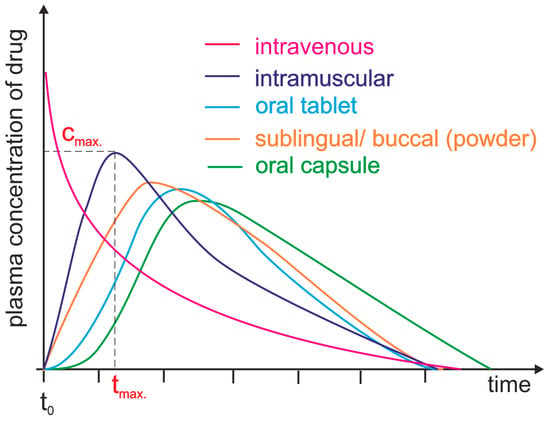
\includegraphics[width=1\linewidth]{images/fig-drug-absorption} \caption{ความเข็มข้นของยาในกระแสเลือดที่เวลาต่างๆ }\label{fig:fig-drug-absorption}
\end{figure}

ในการทำความเข้าใจการเปลี่ยนแปลงของปริมาณข้างต้นเทียบกับเวลา เราสามารถประยุกต์ใช้การสร้างแบบจำลองทางคณิตศาสตร์เพื่อมาใช้อธิบายการเปลี่ยนแปลงของปริมาณต่างๆ ที่เกี่ยวข้อง

\begin{quote}
\textbf{การสร้างแบบจำลองทางคณิตศาสตร์} เป็นกระบวนการอธิบายปัญหาหรือ ปรากฎการต่างๆ ที่เกิดขึ้นในธรรมชาติ โดยปกติแล้วจะอยู่ในรูปของสมการทางคณิตศาสตร์ ซึ่งแบบจำลองทางคณิตศาสตร์นี้จะช่วยให้อธิบายสิ่งต่างๆ ที่เกิดขึ้นในปัญหาหรือปรากฏที่สนใจ
\end{quote}

ตัวอย่างต่อไปนี้จะแสดงถึงแนวคิดในการประยุกต์ของแคลคูลัสที่เกี่ยวข้องกับอัตราการเปลี่ยนแปลงของ

\begin{example}
\protect\hypertarget{exm:exm1}{}\label{exm:exm1}ในการทดลองหนึ่ง นักวิจัยต้องการศึกษาการขยายพันธ์ของแบคทีเรียที่มีการการแบ่งตัวที่เรียกว่า binary fission (การแบ่งตัวแบบทวิภาค) ซึ่งแบคทีเรียจะมีการแบ่งจากหนึ่งเป็นสองเซลเท่าๆ กัน และได้ผลการทำลองดังต่อไปนี้
\end{example}

\begin{figure}
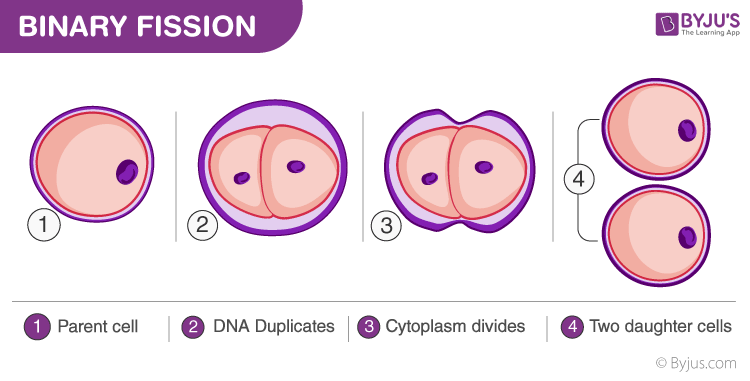
\includegraphics[width=1\linewidth]{images/fig-binary-fission} \caption{กระบวนการแบ่งตัวแบบทวิภาคของแบคทีเรีย}\label{fig:fig-binary-fission}
\end{figure}

(รูปอ้างอิงจาก \href{https://byjus.com/biology/binary-fission/}{BYJU's Learning Website} )

\begin{table}

\caption{\label{tab:bacteria-table}จำนวนของแบคทีเรียที่เวลา t ใดๆ}
\centering
\begin{tabular}[t]{l|r|r|r|r|r|r|r}
\hline
เวลา (10 นาที) & 0 & 1 & 2 & 3 & 4 & 5 & 6\\
\hline
จำนวนแบคทีเรีย & 1 & 2 & 4 & 8 & 16 & 32 & 64\\
\hline
\end{tabular}
\end{table}

ตาราง \ref{tab:bacteria-table} และรูปที่ \ref{fig:population-plot} แสดงการเปลี่ยนแปลงของจำนวนแบคทีเรียที่เวลาใดๆ ในตัวอย่างนี้การเปลี่ยนแปลงของจำนวนของแบคทีเรียที่เวลา \(t\) สามารถเขียนในรูปฟังก์ชัน \(N(t)\) ถ้าให้ \(N_0\) แทนจำนวนของแบคทีเรียตอนเริ่มการทดลอง แล้วแบบจำลองทางคณิตศาสตร์สำหรับการเพิ่มของจำนวนแบคทีเรียจะสามารถเขียนในรูปของสมการ

\begin{equation}
N(t) = N_0 \cdot 2 ^t, \quad t = 0,1,2, \ldots
\label{eq:population-growth}
\end{equation}

ในแบบจำลองทางคณิตศาสตร์นี้การเปลี่ยนแปลงของจำนวนแบคทีเรียที่เวลา \(t\) ใดๆ เพิ่มขึ้นในลักษณะที่เรียกว่า เอกซ์โพเนนเชียล (Exponential Population Growth)

\begin{figure}
\centering
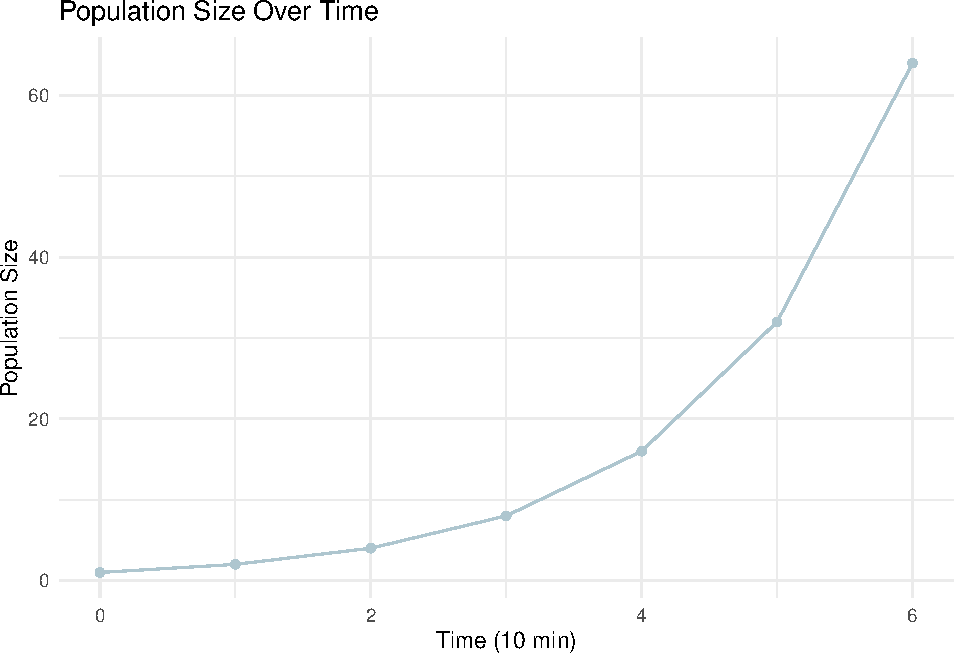
\includegraphics{SCMA104bookdownproj_files/figure-latex/population-plot-1.pdf}
\caption{\label{fig:population-plot}Population Size Over Time}
\end{figure}

\begin{example}
\protect\hypertarget{exm:exm2}{}\label{exm:exm2}ในการสร้างแบบจำลองทางคณิตศาสตร์ ในตัวอย่างของการขยายพันธ์แบคทีเรีย หรือในปัญหาอื่นๆ แทนที่เราจะพยายามหาความสัมพันธ์ หรือฟังก์ชัน \(N(t)\) ในรูปของเวลา \(t\) โดยตรง ถ้าเราทราบกระบวนการที่เกี่ยวข้องกับการอัตราการเปลี่ยนแปลงของตัวแปร \(N(t)\) นั้น เราสามารถนำมาใช้ในการสร้างแบบจำลองทางคณิตศาสตร์ ได้ดังต่อนี้ กระบวนการที่เกี่ยวข้องกับการเปลี่ยนแปลงของจำนวนแบคทีเรีย (การเพิ่มหรือลดลงของแบคทีเรีย) ที่เกิดขึ้นในระหว่างเวลา \(t\) และเวลา \(t + h\) เกิดจากจำนวนแบคทีเรียที่เพิ่มขึ้น (เกิดขึ้นมาใหม่) ในช่วงเวลาดังกล่าว และลดลงจากจำนวนแบคทีเรียที่ลดลง (ตายไป) ในช่วงเวลาดังกล่าวเช่นกัน ซึ่งเราสามารถเขียนในรูปของสมการได้ดังต่อไปนี้
\end{example}

\begin{equation}
   \begin{aligned}
      N(t + h) &= N(t) \\
               &\quad +     \text{จำนวนแบคทีเรียที่เกิดขึ้นใหม่ระหว่าง } t \text{ และ } t+h \\
              &\quad - \text{จำนวนแบคทีเรียที่ตายไประหว่าง } t \text{ และ } t+h
    \end{aligned}          
    \label{eq:population-growth-2}
\end{equation}

ในที่นี้ ``\textbf{การเกิด}'' เราหมายถึงการเพิ่มจำนวนของแบคทีเรียจากหนึ่งเป็นสอง และเราจะกำหนดให้ \(h\) เป็นช่วงเวลาสั้นๆ (ซึ่งเราสามารถใช้ความรู้แคลคูลัสในการสร้างแบบจำลองทางคณิตศาสตร์ในรูปของสมการเชิงอนุพันธ์ (differential equation)) ในสมการ \eqref{eq:population-growth-2} ถ้าเราสมมติว่า การเพิ่มของแบคทีเรียเป็นสัดส่วนกับจำนวนแบคทีเรียที่มีอยู่ในขณะนั้น หรือเขียนในรูปของสมการได้ดังนี้

\[
\text{จำนวนแบคทีเรียที่เกิดใหม่ระหว่าง } t \text{ และ } t + h \approx b \cdot N \cdot h
\]

\[
\text{จำนวนแบคทีเรียที่ตายไประหว่าง } t \text{ และ } t + h \approx m \cdot N \cdot h
\]

โดยที่ค่าคงตัว \(b\) และ \(m\) ในสมการข้างต้น คือ อัตราการเกิด (birth rate) และอัตราการตาย (mortality rate)

เมื่อแทนจำนวนแบคทีเรียที่เกิดใหม่ และตายไประหว่างช่วงเวลาที่กำหนดลงในสมการ \eqref{eq:population-growth-2} จะได้สมการ

\begin{equation}
N(t + h) - N(t) = b\cdot N(t) \cdot h - m\cdot N(t) \cdot h
\label{eq:population-growth-3}
\end{equation}

เราสามารถจัดรูปสมการ \eqref{eq:population-growth-3} ได้ไหมในรูปของ\textbf{อัตราการเปลี่ยนแปลงเฉลี่ย}ของจำนวนแบคทีเรียในช่วงเวลาดังกล่าว ดังนี้

\begin{align}
\frac{N(t + h) - N(t)}{h} &= b\cdot N(t)  - m\cdot N(t)\\
\label{eq:population-growth-4}
\end{align}

ดังนั้น ถ้าเราให้ \(h\) เข้าใกล้ 0 ผ่านการหาค่าลิมิต เราจะได้อัตราการเปลี่ยนแปลงขณะหนึ่ง (instantaneous rate of change) และเขียนได้ในรูปของสมการเชิงอนุพันธ์ ดังนี้

\begin{align}
\frac{dN}{dt} = \lim_{h \rightarrow 0}\frac{N(t + h) - N(t)}{h} &= b\cdot N(t)  - m\cdot N(t)\\
\label{eq:population-growth-5}
\end{align}

ทั้งนี้ในการแก้สมการเชิงอนุพันธ์ \eqref{eq:population-growth-5} เพื่อให้ได้คำตอบที่แสดงจำนวนแบคทีเรีย \(N(t)\) ในรูปของฟังก์ชันของ \(t\) เราจะต้องกำหนดเงื่อนไขเพิ่มเติมที่เกี่ยวข้องกับจำนวนแบคทีเรีย \(N(t)\) ที่เวลา \(t\) หนึ่ง โดยทั่วไปเราจะกำหนดค่าเริ่มต้นของจำนวนแบคทีเรียที่ \(t = 0\) ดังนั้น ถ้าเรากำหนดเงื่อนไขเริ่มต้น (initial condition)

\begin{equation}
N(0) = N_0
\label{eq:population-growth-6}
\end{equation}

เราสามารถหาคำตอบของสมการเชิงอนุพันธ์ที่มีเงื่อนไขเริ่มต้นโดยวิธีการหาปริพันธ์ (Integration) ได้คำตอบของสมการดังนี้

\begin{equation}
N(t) = N_0 e^{(b-m)t}
\label{eq:population-growth-7}
\end{equation}

\begin{example}
\protect\hypertarget{exm:exm3}{}\label{exm:exm3}

ในการทดลองเลี้ยงยีสต์ในขวดทดลองที่มีอาหารเลี้ยงยีสต์ในปริมาณที่เหมาะสม ผู้ทำการทดลองสนใจที่จะประมาณค่าของยีสต์โดยอาศัยแบบจำลองการเปลี่ยนแปลงของประชากรที่อธิบายด้วยสมการ \eqref{eq:population-growth-7} กำหนดให้

\begin{itemize}
\item
  ภายใต้สภาวะของการทดลองที่เหมาะสม ยีสต์จะแบ่งตัวทุกๆ 90 นาที
\item
  ยีสต์มีครึ่งชีวิตเท่ากับ 1 สัปดาห์
\end{itemize}

จากข้อมูลดังกล่าว จงแสดงวิธีทำเพื่อหาคำตอบจากคำถามต่อไปนี้

\begin{enumerate}
\def\labelenumi{\arabic{enumi}.}
\item
  จงประมาณค่าของอัตราการเกิด \(b\) (1/ชั่วโมง) และอัตราการตาย \(m\) (1/ชั่วโมง)
\item
  เขียนแบบจำลองทางคณิตศาสตร์โดยใช้ค่า \(b\) และ \(m\) ที่ประมาณค่าได้ (สมการ \eqref{eq:population-growth-7})
\item
  ใช้เครื่องมือที่นักศึกษามีอยู่ในการวาดกราฟแสดงความสัมพันธ์ของจำนวนยีสต์ที่เวลาต่างๆ
\item
  เปรียบเทียบผลลัพธ์ที่ได้กับรูปภาพแสดงการเปลี่ยนแปลงของยีสต์จากการทดลองในห้องปฏิการ ตามรูปที่ \ref{fig:fig-yeast-cells} (รูปภาพอ้างอิงจาก \href{https://homework.study.com/explanation/a-graph-of-a-population-of-yeast-cells-in-a-new-laboratory-culture-as-a-function-of-time-is-shown-a-describe-how-the-rate-of-population-increase-varies-b-when-is-this-rate-highest-c-on-what-intervals-is-the-population-function-concave-upward-or-d.html}{https://homework.study.com/})
\end{enumerate}

\end{example}

\begin{figure}

{\centering 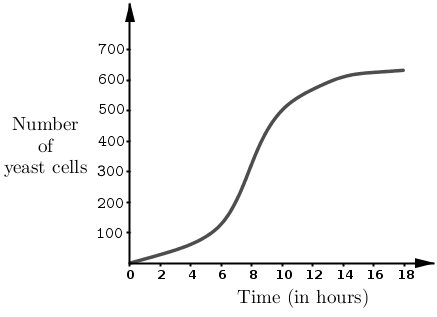
\includegraphics[width=0.5\linewidth]{images/fig-yeast-cells} 

}

\caption{กราฟการเจริญเติบโตของเซลล์ยีสต์}\label{fig:fig-yeast-cells}
\end{figure}

\begin{example}
\protect\hypertarget{exm:exm4}{}\label{exm:exm4}

จงใช้อินเทอร์เน็ตเพื่อค้นหาตัวอย่างแบบจำลองทางคณิตศาสตร์ที่อธิบายโดยสมการเชิงอนุพันธ์หรือระบบสมการเชิงอนุพันธ์ ข้อมูลที่ต้องการประกอบด้วย

\begin{enumerate}
\def\labelenumi{\arabic{enumi}.}
\item
  ค้นหาหน้าเว็บที่ให้ข้อมูลเกี่ยวกับแบบจำลองทางคณิตศาสตร์ในปัญหาที่นักศึกษาสนใจ
\item
  จดบันทึก URL ของหน้าเว็บ
\item
  เขียนสรุปสั้นๆ ว่าโมเดลนี้ใช้เพื่ออะไร
\end{enumerate}

\end{example}

\textbf{วิธีทำ}

ตัวอย่างของแบบจำลองทางคณิตศาสตร์ที่ได้จากการสืบค้นข้อมูลอินเทอร์เน็ตจาก

\begin{itemize}
\item
  \href{https://sites.northwestern.edu/recalculated/2019/05/05/calculus-in-medicine/}{CALCULUS IN MEDICINE (https://sites.northwestern.edu/recalculated/2019/05/05/calculus-in-medicine/)}
\item
  \href{https://ns.mahidol.ac.th/english/th/departments/MN/th/doc/km54/เภสัชจลนศาสตร์\%20(Pharmacokinetics).pdf}{เภสัชจลนศาสตร์ (Pharmacokinetics) และ เภสัชพลศาสตร์ (Pharmacodynamics) (https://ns.mahidol.ac.th/english/th/departments/MN/th/doc/km54/เภสัชจลนศาสตร์\%20(Pharmacokinetics).pdf)}
\end{itemize}

แบบจำลองทางคณิตศาสตร์จำลองการเปลี่ยนแปลงของความเข้มข้นของยา \(c\) ณ เวลา \(t\) โดยที่กำหนดขนาดยา (drug dosage) เท่ากับ \(d\)

\[
\frac{dc}{dt} = \frac{k_a}{k_a - k_e}\left[ k_a \cdot d \cdot b \cdot e^{-at} - k_e \cdot c \cdot v \right]
\]

โดยที่

\begin{itemize}
\item
  \(k_a\) คือ ค่าคงตัวของการดูดซึมยา
\item
  \(k_e\) คือ ค่าคงตัวของการกำจัดยา
\item
  \(v\) แทน ปริมาตรของยาในร่างกาย
\item
  \(b\) แทน สัดส่วนของปริมาณยาที่ถูกดูดซึมเข้าไปในร่างกายเทียบกับขนาดของยา
\end{itemize}

ตามหลักเภสัชจลนศาสตร์ เมื่อได้รับยาเข้าสู่ร่างกาย จะมีกระบวนการดูดซึมยา การกระจายตัวของยา การเปลี่ยนแปลงยา และการขับถ่ายยาออกจากร่างกาย

\begin{figure}
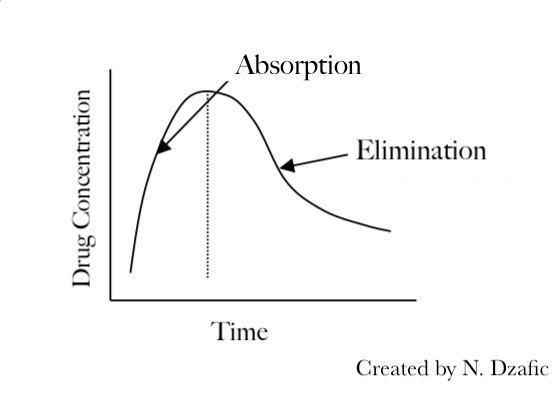
\includegraphics[width=0.5\linewidth]{images/fig-drub-absorption} \caption{การเปลี่ยนแปลงความเข้มข้นของยาในระยะการดูดซึม และการกำจัดออกจากร่างกาย}\label{fig:fig-drub-absorption}
\end{figure}

การสร้างแบบจำลองทางคณิตศาสตร์จะมีประโยชน์ที่สำคัญที่ทำให้ผู้เชี่ยวชาญด้านยาสามารถกำหนดขนาดของยาที่เหมาะสม อย่างต่อเนื่องเป็นระยะเวลาที่เพียงพอกับการรักษา เพื่อให้ได้ผลการรักษาที่ดีที่สุด

โดยสรุป แคลคูลัสและสมการเชิงอนุพันธ์เป็นเครื่องมือสำคัญในการทำความเข้าใจว่าสิ่งต่างๆ เปลี่ยนแปลงไปอย่างไรและ แคลคูลัสช่วยให้เราวิเคราะห์อัตราการเปลี่ยนแปลงและพื้นที่ใต้เส้นโค้ง ในขณะที่สมการเชิงอนุพันธ์ช่วยให้เราสร้างแบบจำลองระบบที่ซับซ้อนในสาขาต่างๆ เช่น ฟิสิกส์ วิศวกรรม เศรษฐศาสตร์ และชีววิทยา แนวคิดทางคณิตศาสตร์เหล่านี้มีความสำคัญต่อการแก้ปัญหาในโลกแห่งความเป็นจริง เมื่อโลกของเราก้าวหน้ามากขึ้น ความสำคัญของแคลคูลัสและสมการเชิงอนุพันธ์ก็จะเพิ่มขึ้นอย่างต่อเนื่อง ซึ่งสนับสนุนความก้าวหน้าทางวิทยาศาสตร์และเทคโนโลยี

\chapter{ลิมิต (Limits)}\label{uxe25uxe21uxe15-limits}

อาจกล่าวได้ว่า วิชาแคลคูลัส
ถือกำเนิดขึ้นมาจากความพยายามในการแก้ปัญหาทางเรขาคณิตบนระนาบ 2 ปัญหาหลักๆ คือ

\begin{itemize}
\item
  การหาเส้นตรงที่สัมผัสเส้นโค้งที่กำหนดให้

  กำหนดฟังก์ชัน (function) \(f\) และกำหนดจุด \(P(x_{0},y_{0})\) บนกราฟ
  \(y = f(x)\) จงหาสมการของเส้นตรงที่สัมผัสกราฟ \(y = f(x)\) ที่จุด \(P\)
\item
  การหาพื้นที่ของบริเวณที่กำหนดให้

  กำหนด function \(f\) และช่วง \([a,b]\) ในโดเมนของ \(f\)
  จงหาพื้นที่ที่ถูกปิดล้อมด้วยแกน \(X\) และกราฟ \(y = f(x)\) สำหรับ \(x \in [a,b]\)
\end{itemize}

แนวความคิดในการแก้ปัญหาทั้งสอง นำไปสู่การศึกษาเรื่อง ลิมิต (Limits)
ซึ่งเป็นพื้นฐานของวิชาแคลคูลัสนั่นเอง

แต่ในปัจจุบันเราพบว่าวิชาแคลคูลัสมีประโยชน์ในการช่วยแก้ปัญหาในสาขาวิชาต่าง ๆ มากมาย เช่น
เราจะพบในการศึกษาวิชานี้ว่า แคลคูลัสมีบทบาทในการแก้ปัญหาต่อไปนี้

\begin{itemize}
\item
  โดยทั่วไป ยาชนิดฉีดจะต้องใช้เวลาระยะหนึ่งหลังจากฉีดเข้าสู่ร่างกาย
  ในการที่จะไหลเวียนในกระแสโลหิต จนกระทั่งมีความเข้มข้นสูงสุด สมมุติว่า
  ยาฉีดชนิดหนึ่งหลังจากฉีดเข้าสู่ร่างกายนาน \(t\) ชั่วโมง จะมีความเข้มข้นเป็น
  \(C(t) = 0.15(e^{-0.18t}-e^{-1.2t})\) มิลลิกรัมต่อมิลลิลิตร จงหาว่า
  นานเท่าใดหลังจากฉีดยา จึงจะมีความเข้มข้นของยา ในกระแสโลหิตสูงที่สุด
\item
  เราอาจประมาณได้อย่างมีเหตุผลว่า artery มีรูปร่างที่เป็นผลมาจากการหมุนรอบแกน
  ของเส้นโค้งในระนาบ โดยในสภาวะนิ่ง รัศมีของ artery มีค่าคงที่เท่ากับ 1 หน่วย
  (รูปทรงกระบอก) แต่ในขณะที่หัวใจสูบฉีดโลหิตผ่าน artery artery จะพองตัวออก
  ทำให้รัศมีเปลี่ยนไปตามสมการ \(R(x) = 1+0.4x-0.04x^{2}\) หน่วย เมื่อ
  \(0 \leq x\leq 10\) เป็นตำแหน่งบนแนวยาวของ artery จงหาว่า ปริมาณโลหิตที่อยู่ใน
  artery ขณะที่หัวใจสูบฉีดโลหิตผ่านเข้ามาเป็นกี่เท่าของความจุโลหิตในสภาวะนิ่ง
\item
  ความก้าวหน้าในทางการแพทย์ และเทคโนโลยีปัจจุบัน
  ทำให้มีการประดิษฐ์อุปกรณ์ช่วยในการรักษาโรคเบาหวานชิ้นหนึ่งขึ้น
  อุปกรณ์นี้มีลักษณะเป็นแคปซูล ซึ่งเมื่อฝังอุปกรณ์นี้ภายในร่างกายแล้ว
  มันจะหลั่งสารอินซูลินที่บรรจุอยู่ภายใน ออกสู่กระแสโลหิต โดยมีอัตราการหลั่งเป็น
  \(f\left( t\right) =0.5te^{-0.09t}\) ลูกบาศก์เซนติเมตรต่อวัน เมื่อ t คือ
  เวลาเป็นวัน นับจากอุปกรณ์เริ่มทำงาน จงหาว่า
  แพทย์จะต้องสั่งให้บรรจุอินซูลินในแคปซูลเป็นปริมาณเท่าใด
  เพื่อให้อุปกรณ์นี้สามารถให้อินซูลินแก่ผู้ป่วยได้นาน 3 เดือน
\item
  การหาเส้นตรงที่สัมผัสเส้นโค้ง \(y = f(x)\) ณ จุด \(P_{0}(x_{0},y_{0})\)
\end{itemize}

\begin{figure}

{\centering 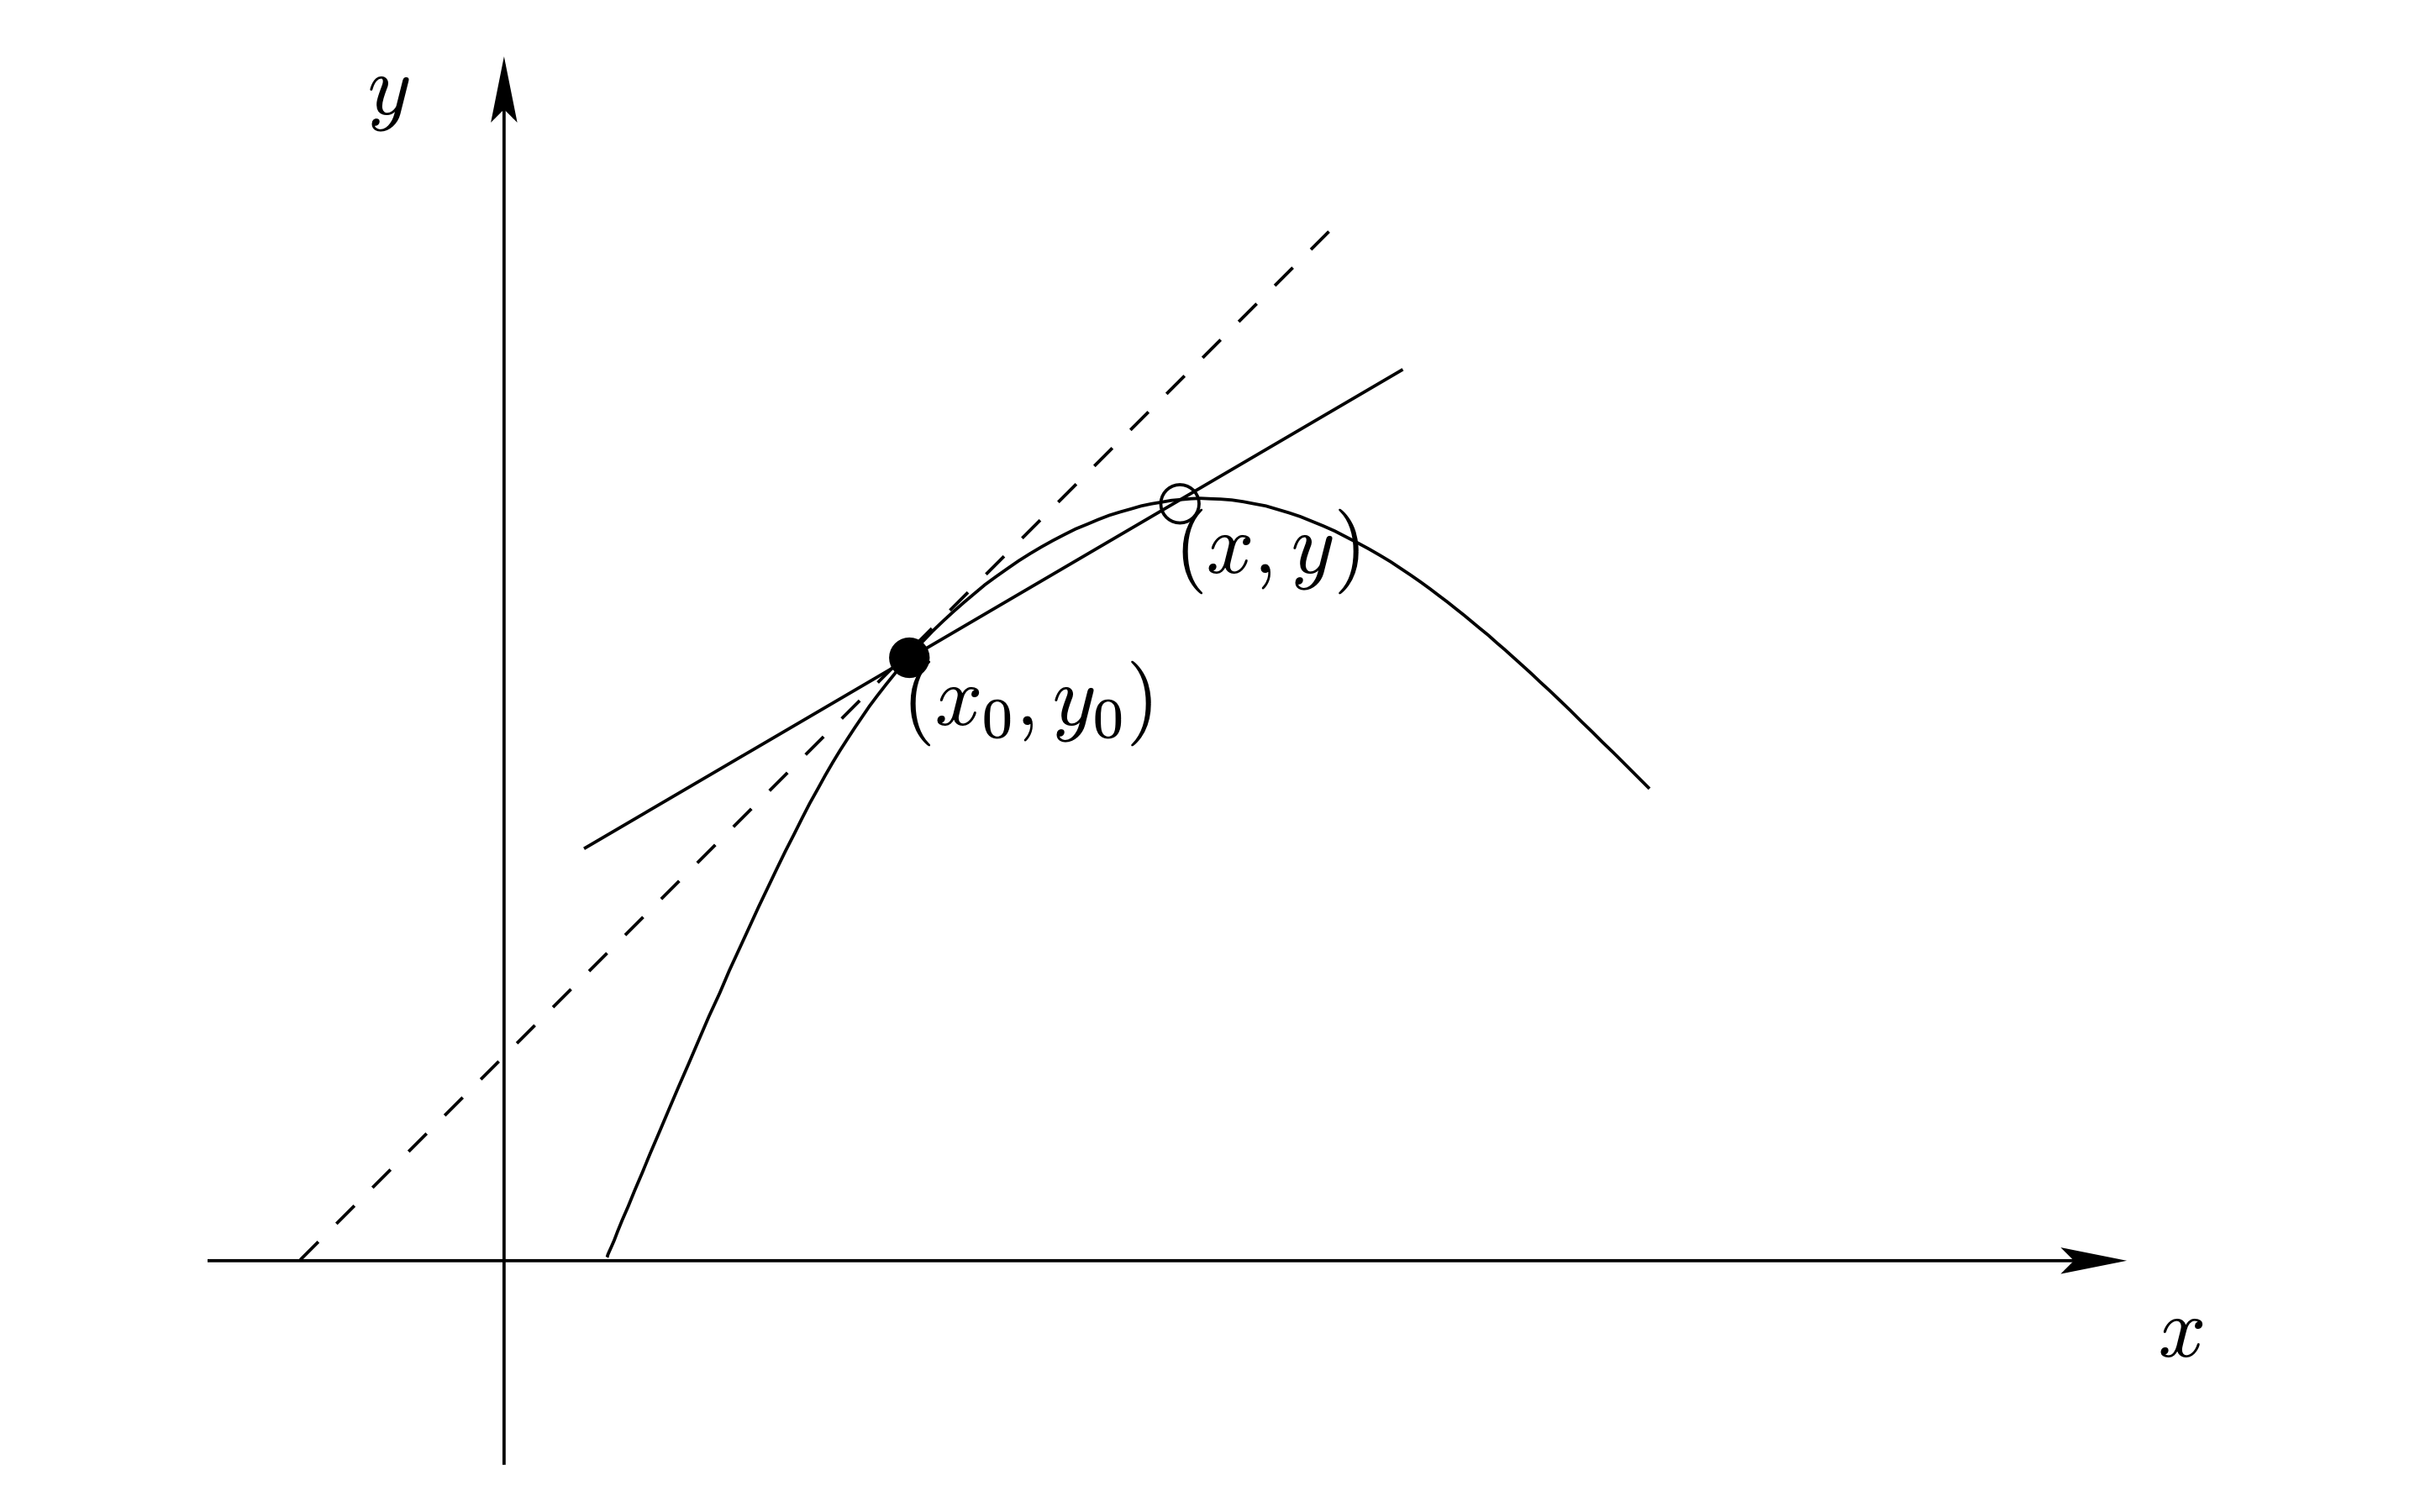
\includegraphics[width=0.5\linewidth]{images/fig-tangent-line} 

}

\caption{การหาเส้นตรงที่สัมผัสเส้นโค้ง}\label{fig:fig-tangent-line}
\end{figure}

ขั้นตอนสรุปการหาเส้นตรงที่สัมผัสเส้นโค้ง \ref{fig:fig-tangent-line}

\begin{enumerate}
\def\labelenumi{\arabic{enumi}.}
\item
  เลือกจุดอื่นบนกราฟ เรียกจุดนี้ว่า \(P(x,y)\)
\item
  ลากเส้นผ่าน \(PP_{0}\)
\item
  ทำซ้ำโดยเลือกจุด P ให้ใกล้ \(P_{0}\) มากขึ้น
\item
  เส้น \(PP_{0}\) ที่ได้จะ ``เข้าใกล้'' เส้นสัมผัสมากขึ้นทุกที
\end{enumerate}

\begin{itemize}
\tightlist
\item
  การหาพื้นที่ ``ใต้กราฟ'' ระหว่าง x = a กับ x = b
\end{itemize}

\begin{figure}

{\centering 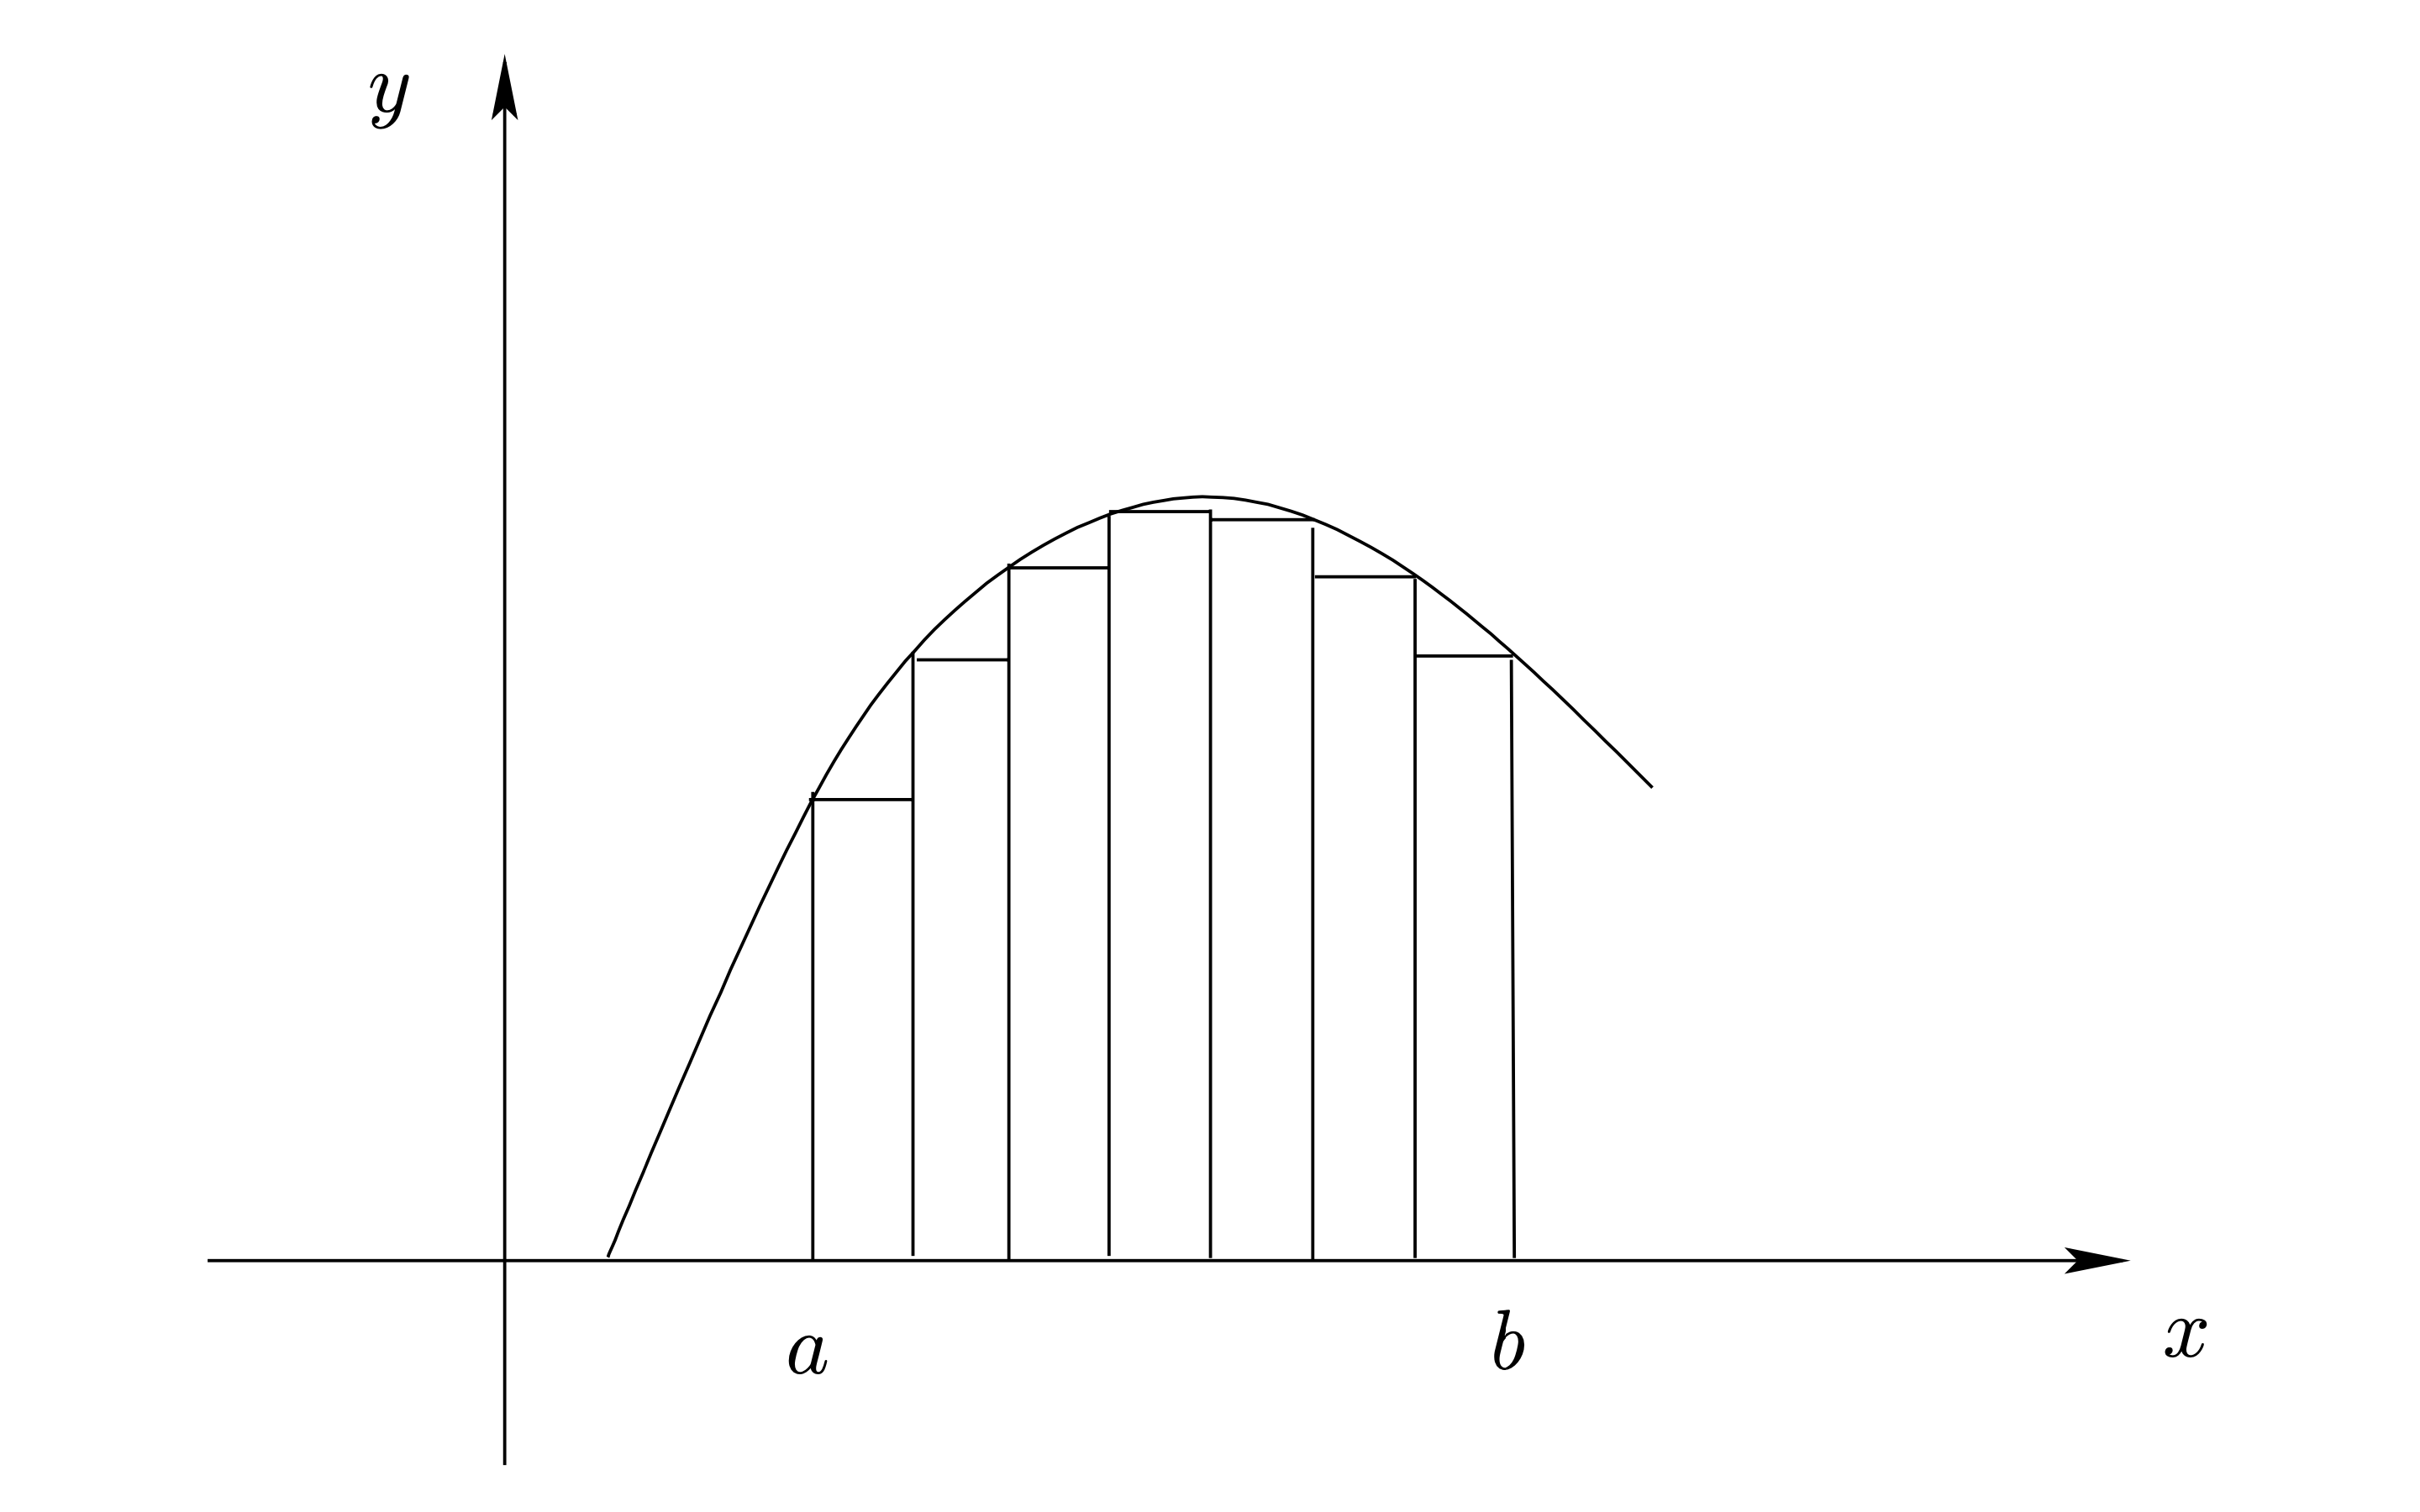
\includegraphics[width=0.5\linewidth]{images/fig-area-under-curve} 

}

\caption{การหาพื้นที่ใต้กราฟ}\label{fig:fig-area-under-curve}
\end{figure}

ขั้นตอนเบื้องต้นสำหรับการหาพื้นที่ใต้กราฟ

\begin{enumerate}
\def\labelenumi{\arabic{enumi}.}
\tightlist
\item
  แบ่ง \([a,b]\) เป็นช่วงเล็กๆ
\item
  หาพื้นที่รวมของสี่เหลี่ยมผืนผ้าทั้งหมด
\item
  ทำซ้ำๆ โดยแบ่งช่วงให้เล็กมากขึ้น
\item
  พื้นที่ที่ได้จะ ``เข้าใกล้'' พื้นที่ที่ต้องการมากขึ้นทุกที
\end{enumerate}

\begin{example}
\protect\hypertarget{exm:ex-limit-1}{}\label{exm:ex-limit-1}จงหาสมการของเส้นสัมผัสกราฟ \(y=-x^{2}+6x-2\) ณ จุด \(P_{0}(2,6)\)
\end{example}

\textbf{วิธีทำ} เลือกจุด \(P(x,y)\) โดยที่ \(x \neq 2\) และลากเส้น \(PP_{0}\) จะได้ว่า
ความชันของ \(PP_{0}\) เท่ากับ

\begin{equation}
  \begin{aligned}
    \frac{y-6}{x-2} &= \frac{-x^{2}+6x-8}{x-2} \\
                    &=-\frac{\left( x-2\right) \left( x-4\right) }{x-2} \\
                    &=4-x
  \end{aligned}
\end{equation}

ถ้า \(P\) อยู่ใกล้ \(P_{0}\) มากขึ้น ค่า x ย่อมเกือบเป็น 2 ดังนั้น ความชันของ \(PP_{0}\)
จึงเข้าใกล้ \(4-2 = 2\) มากขึ้นเรื่อย ๆ เส้นสัมผัสจึงควรมีความชันเป็น 2 และสมการเส้นสัมผัส
คือ \(y-6=2\left( x-2\right)\)

\begin{figure}

{\centering 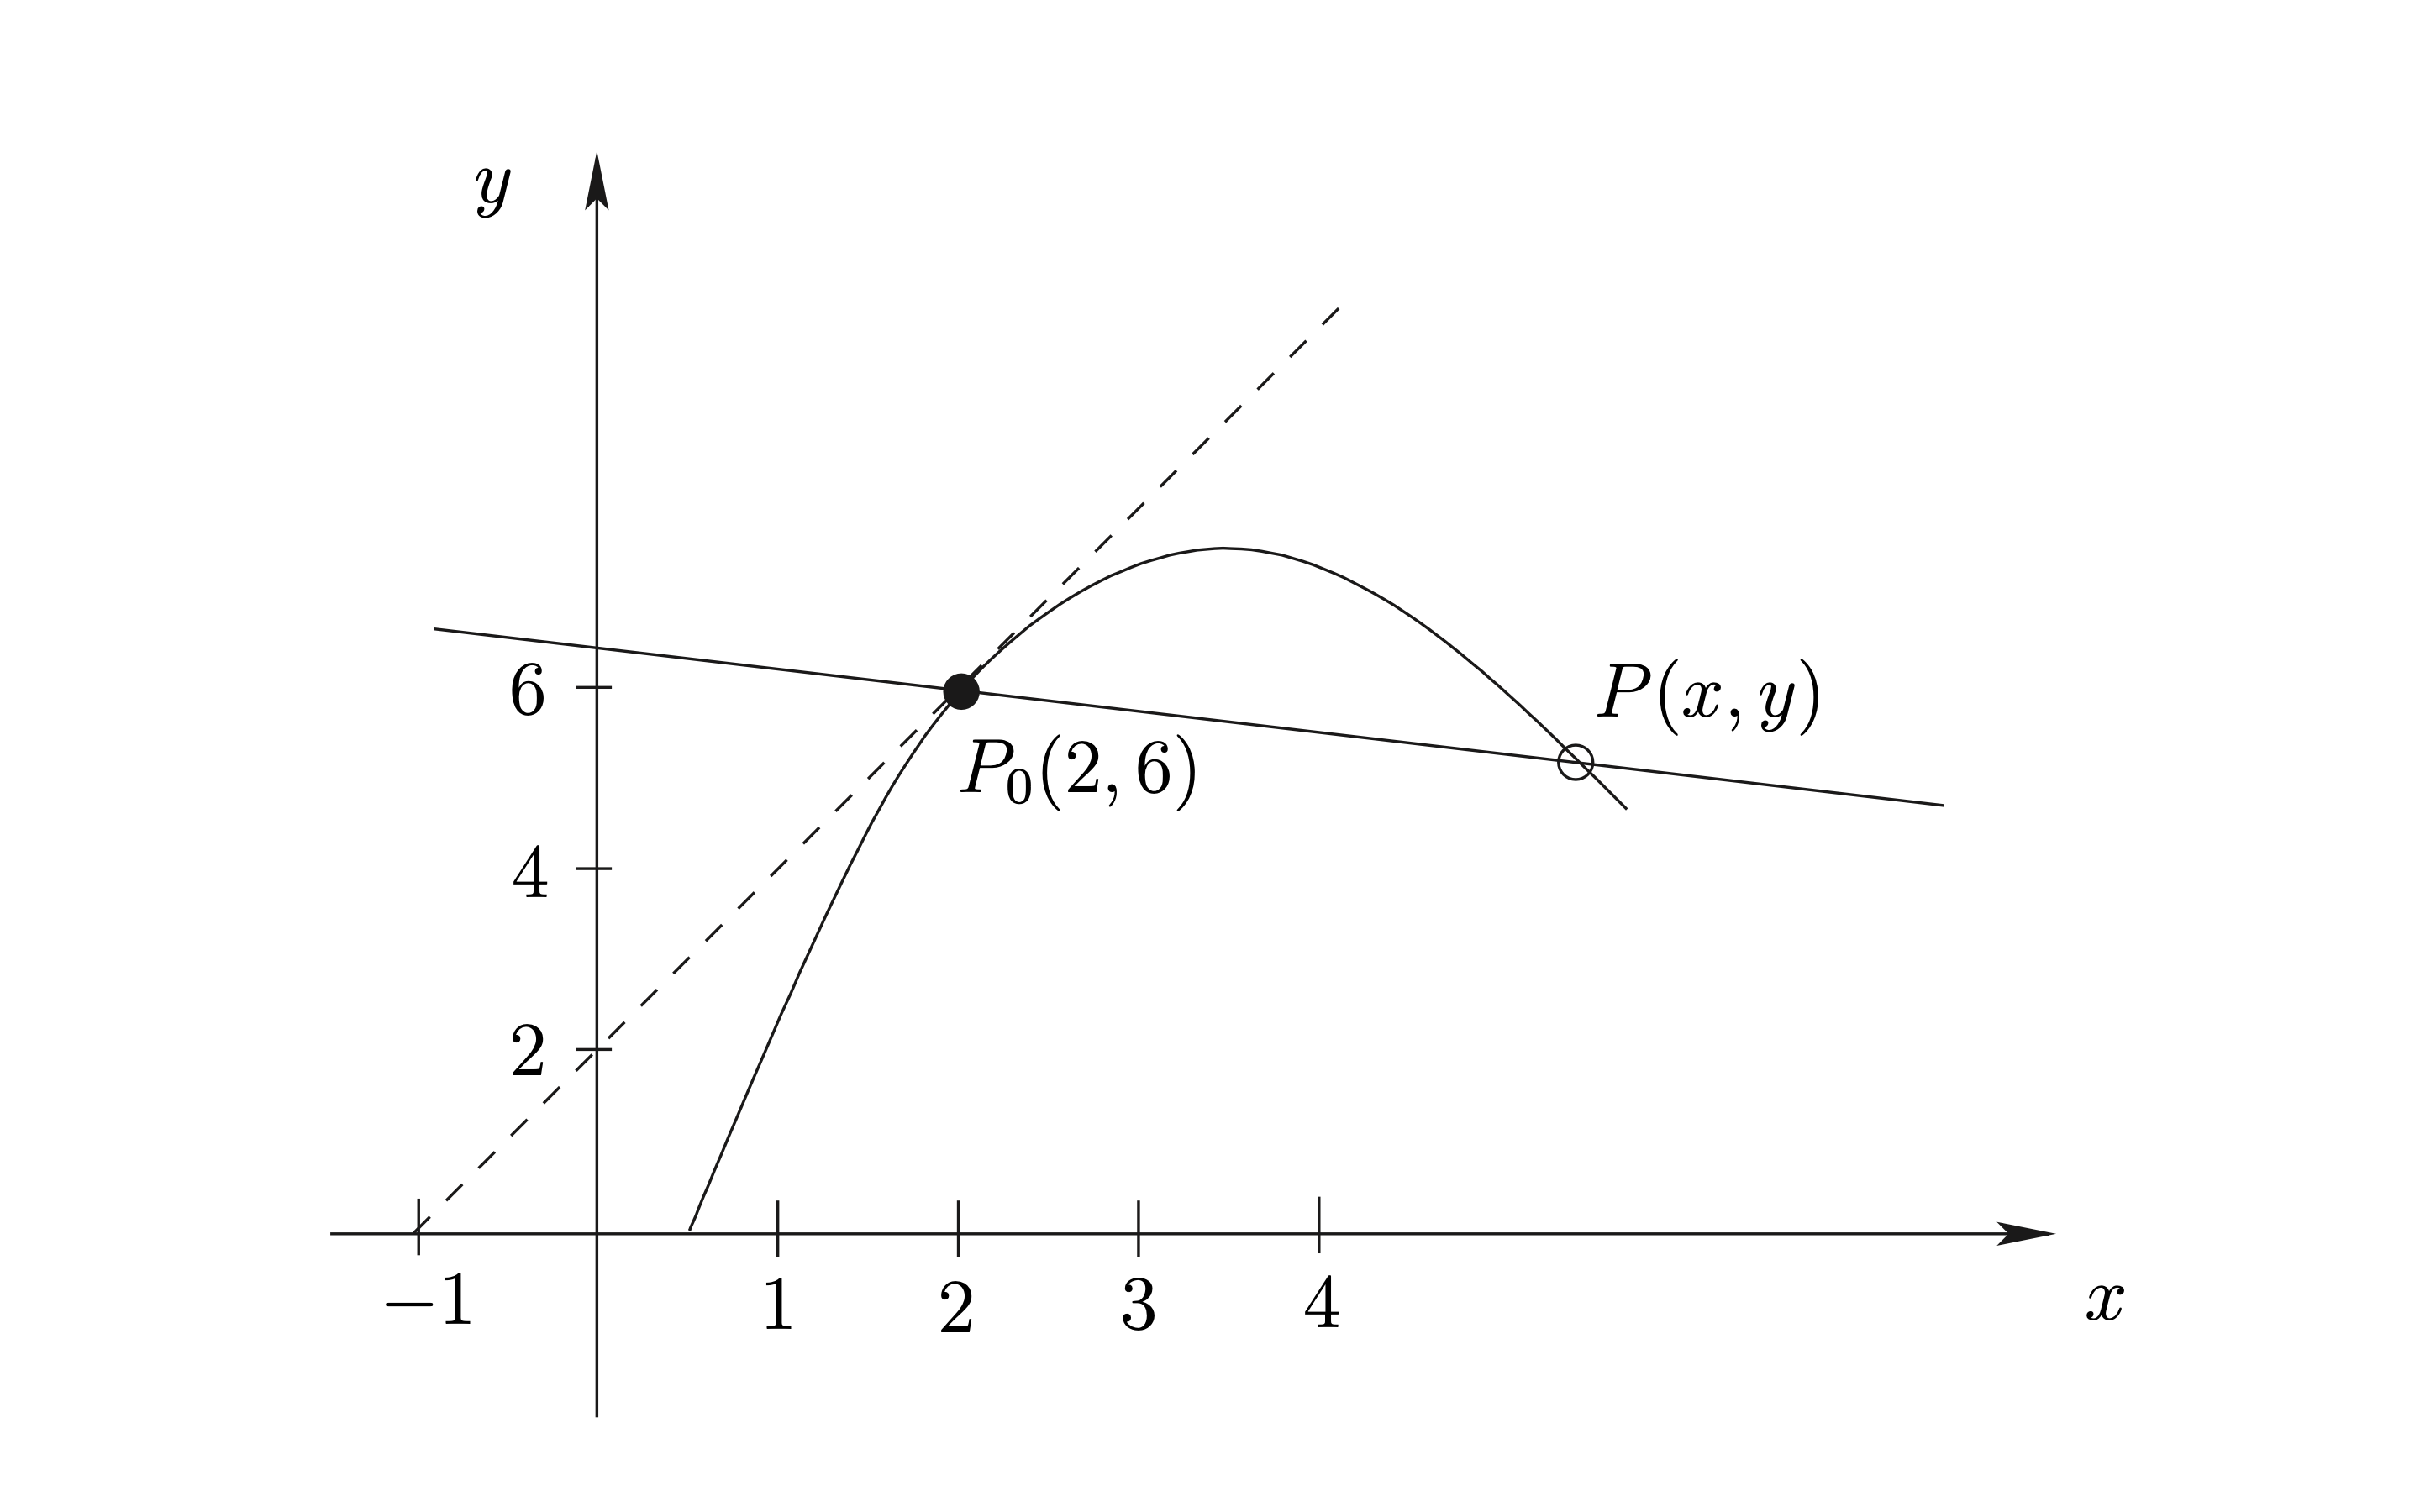
\includegraphics[width=0.5\linewidth]{images/fig-tangent-line-2} 

}

\caption{การหาเส้นตรงที่สัมผัสเส้นโค้ง \(y=-x^{2}+6x-2\)}\label{fig:fig-tangent-line-2}
\end{figure}

จะเห็นว่า ในตัวอย่าง \ref{exm:ex-limit-1} นี้ เราสนใจพฤติกรรมของ function

\(\frac{-x^{2}+6x-8}{x-2}\) เมื่อ \(x \neq 2\) แต่มีค่าใกล้ 2 มาก ๆ นี่คือ ที่มาของเรื่อง

\begin{definition}
\protect\hypertarget{def:def-limit}{}\label{def:def-limit}ให้ \(f : D_{f}\rightarrow R\) โดยที่ \(D_{f}\subseteq R\) และให้ \(a \in R\)
โดยที่มีช่วง \((a,b)\) บางช่วงที่
\(\left( a,b\right) \subseteq D_{f}\left( b>a\right)\)

เรากล่าวว่า ``ลิมิต (limit) ของ \(f(x)\) เมื่อ x เข้าใกล้ a ทางขวา
หาค่าได้และมีค่าเท่ากับจำนวนจริง L'' ถ้า ``ไม่ว่าเราจะกำหนดบริเวณรอบ ๆ \(L\)
ไว้แคบเพียงใด เมื่อเราพิจารณาค่าของ \(f(x)\) สำหรับค่า \(x\) ที่มากกว่า a โดยที่ให้ค่า ของ
\(x\) ลดลงเรื่อย ๆ จนถีงจุดหนึ่ง ค่าของ \(f(x)\) จะอยู่ในบริเวณรอบ ๆ \(L\) ที่เรากำหนดไว้นั้น
และยังคงเป็นเช่นนี้สำหรับ \(x\) อื่น ๆ ที่น้อยกว่านั้น (แต่มากกว่า \(a\) ) ทั้งหมดด้วย''

ในทำนองเดียวกัน ถ้าเราพิจารณาพฤติกรรมของ function สำหรับ \(x\) ที่น้อยกว่า \(a\) จะได้
limit ทางซ้าย ดังนี้ ให้ \(f : D_{f}\rightarrow R\) โดยที่ \(D_{f}\subseteq R\)
และให้ \(a \in R\) โดยที่มีช่วง \((b,a)\) บางช่วงที่
\(\left( b,a\right) \subseteq D_{f}\left( b<a\right)\)

เรากล่าวว่า ``limit ของ \(f(x)\) เมื่อ \(x\) เข้าใกล้ a ทางซ้าย หาค่าได้
และมีค่าเท่ากับจำนวนจริง \(L\)'' ถ้า ``ไม่ว่าเราจะกำหนดบริเวณรอบ ๆ \(L\) ไว้แคบเพียงใด

เมื่อเราพิจารณาค่าของ \(f(x)\) สำหรับค่า \(x\) ที่น้อยกว่า \(a\) โดยที่ให้ค่า ของ \(x\)
เพิ่มขึ้นเรื่อย ๆ จนถีงจุดหนึ่ง ค่าของ \(f(x)\) จะอยู่ในบริเวณรอบ ๆ \(L\) ที่เรากำหนดไว้นั้น
และยังคงเป็นเช่นนี้สำหรับ \(x\) อื่น ๆ ที่มากกว่านั้น (แต่น้อยกว่า \(a\) ) ทั้งหมดด้วย''
\end{definition}

\begin{figure}

{\centering 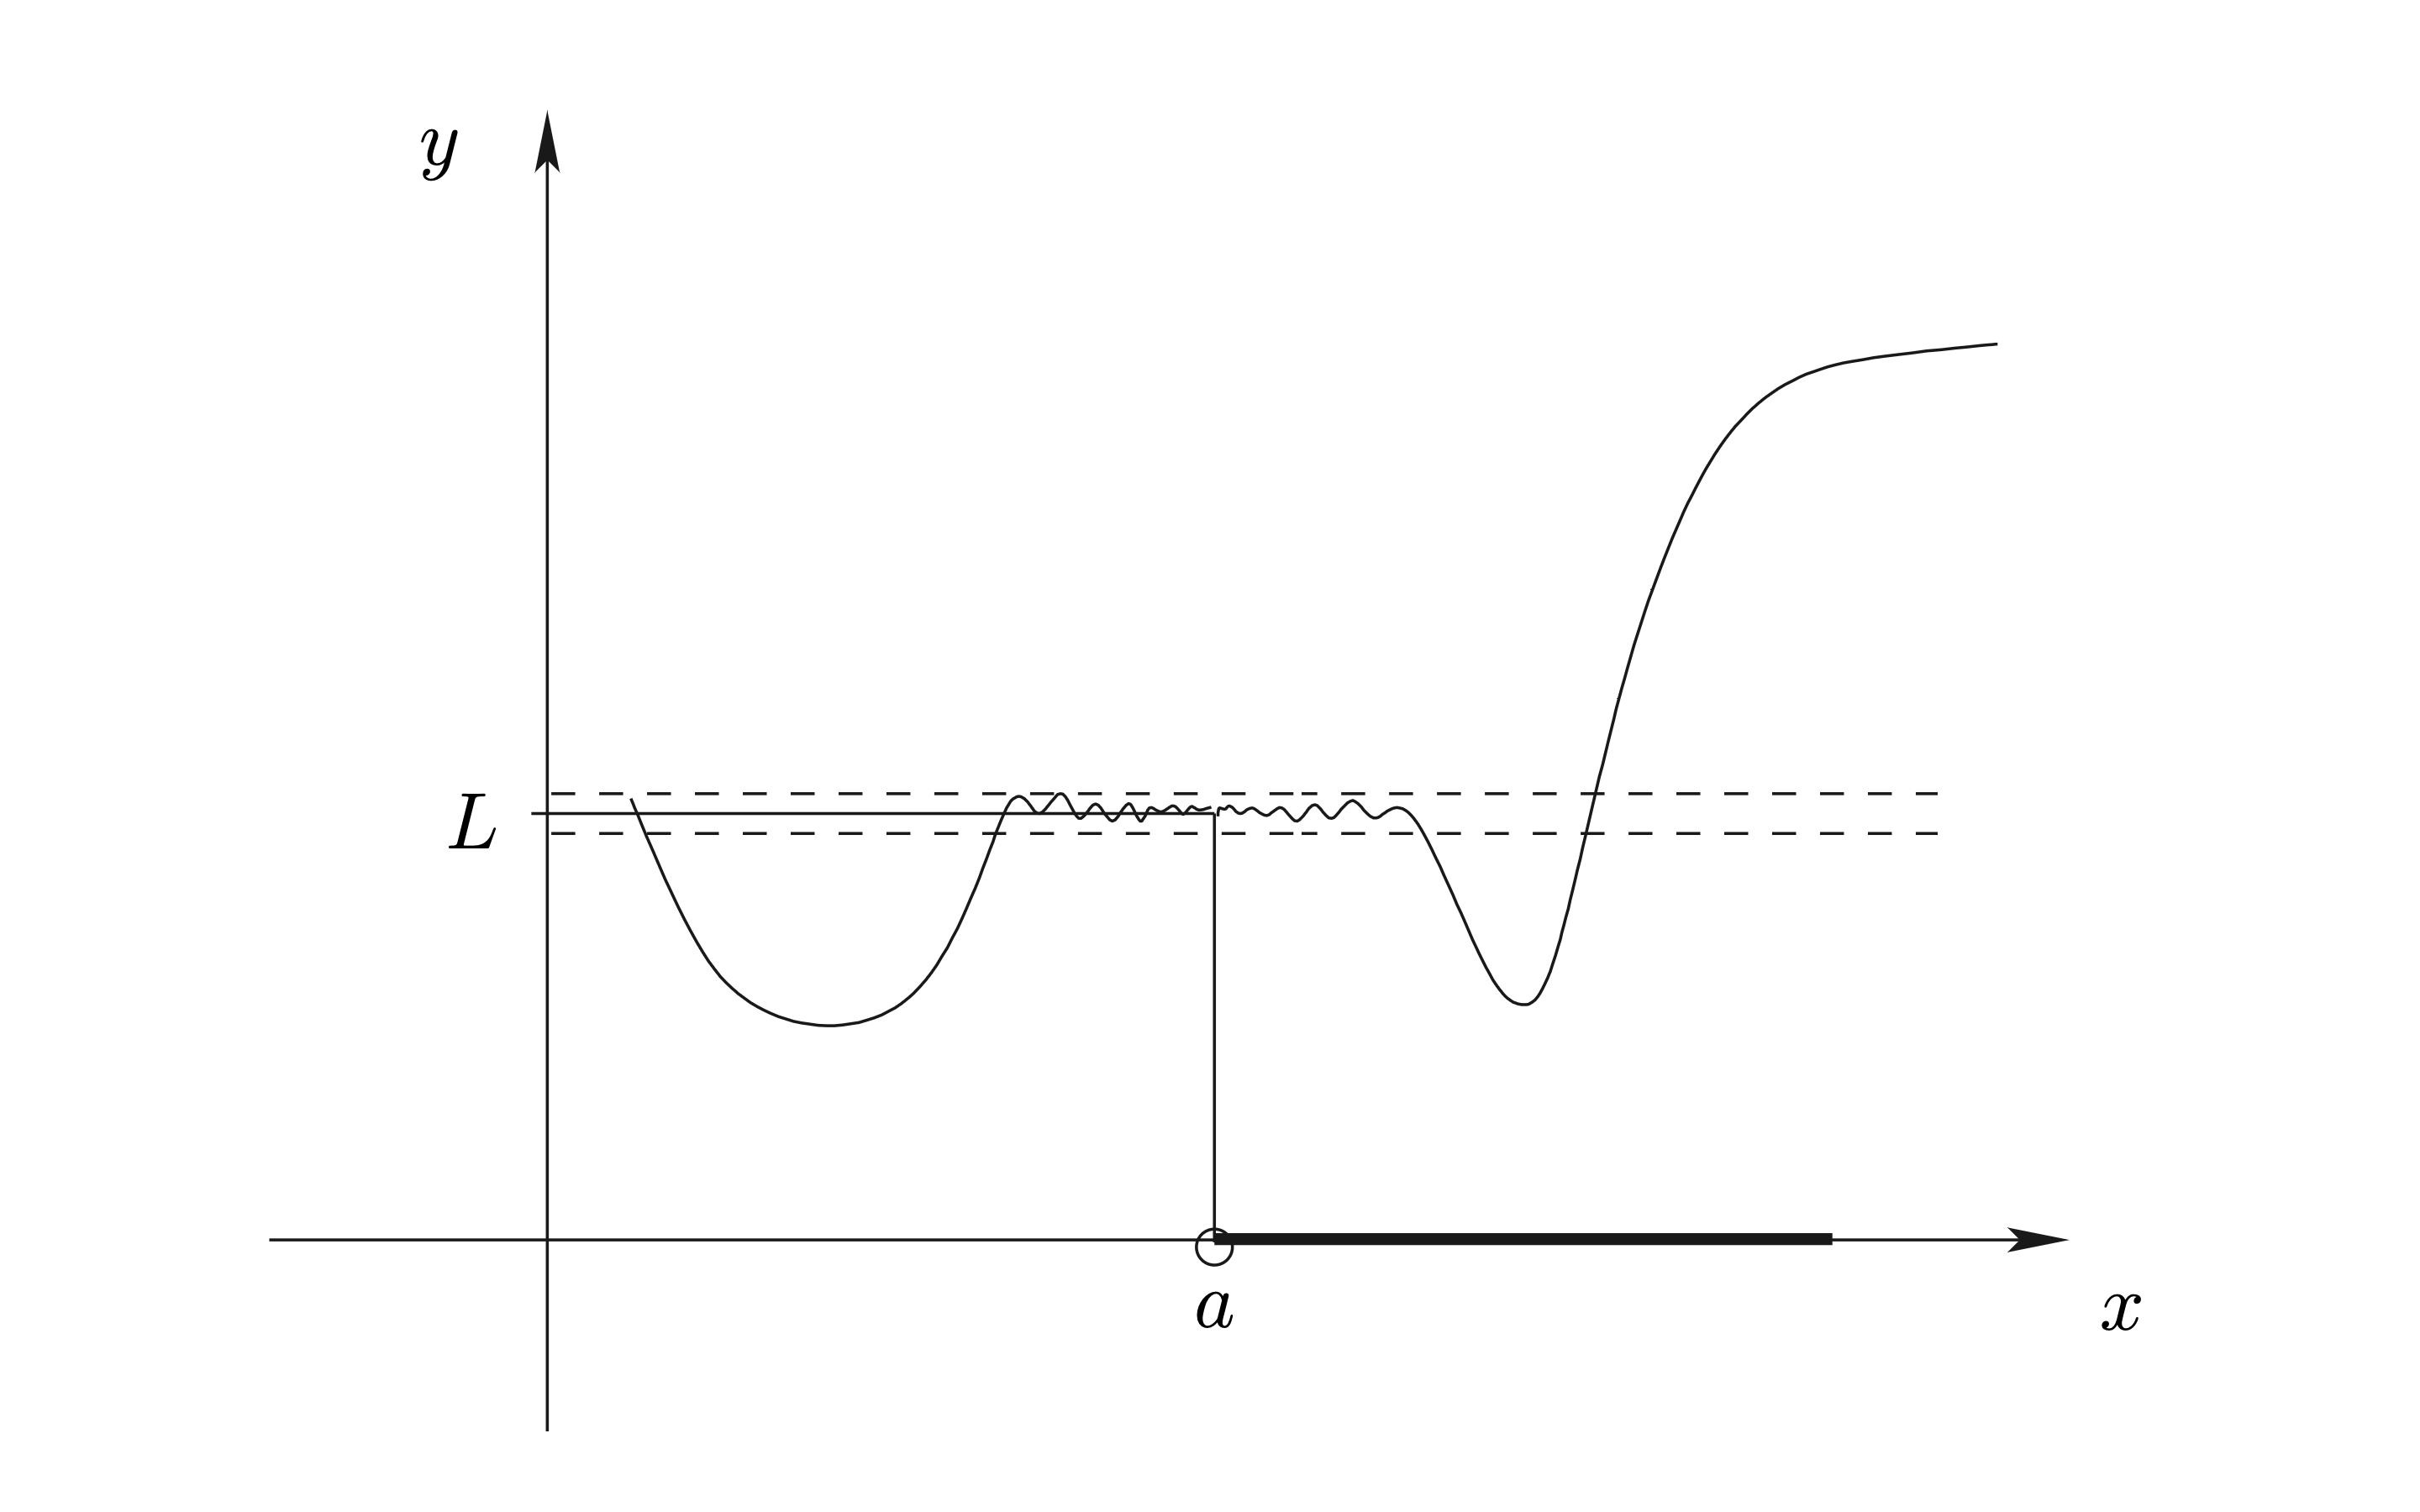
\includegraphics[width=0.5\linewidth]{images/fig-right-limit} 

}

\caption{ลิมิตทางขวา}\label{fig:fig-right-limit}
\end{figure}

\begin{figure}

{\centering 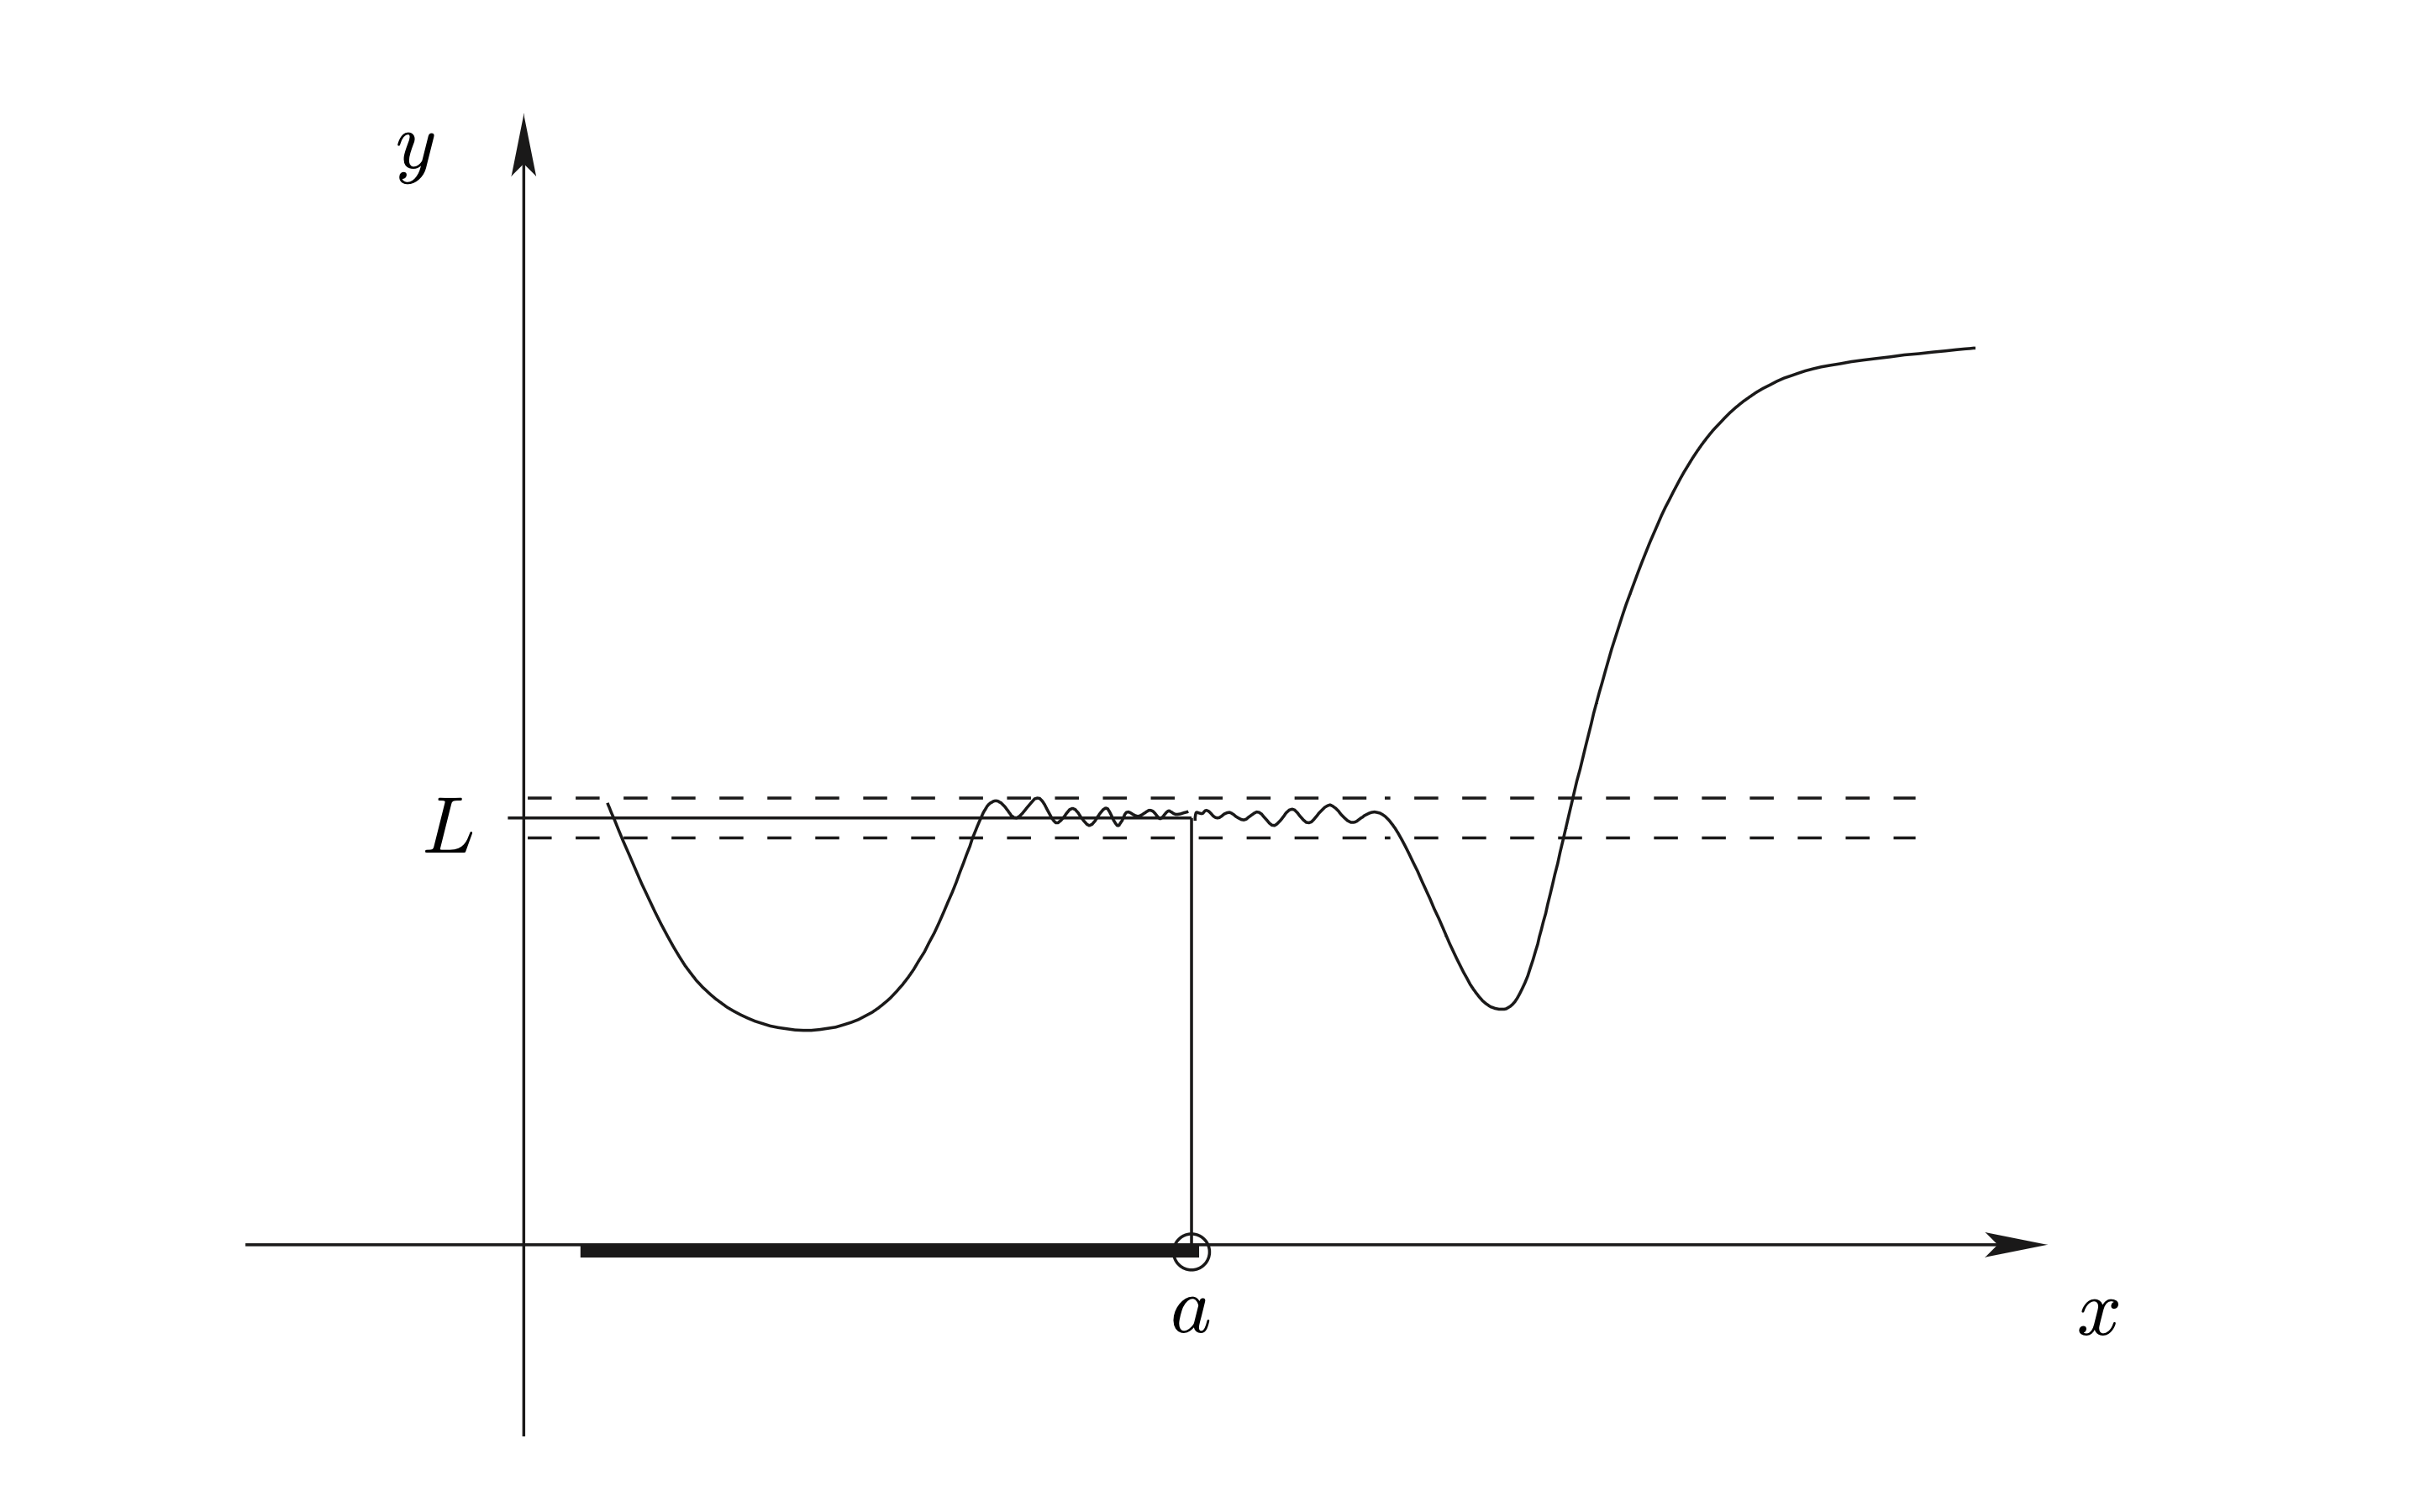
\includegraphics[width=0.5\linewidth]{images/fig-left-limit} 

}

\caption{ลิมิตทางซ้าย}\label{fig:fig-left-limit}
\end{figure}

เราใช้สัญลักษณ์ \(\underset{x\rightarrow a^{+}}{\lim}f(x)\) แทนข้อความ ``limit
ของ \(f(x)\) เมื่อ \(x\) เข้าใกล้ a ทางขวา'' และใช้สัญลักษณ์
\(\underset{x\rightarrow a^{-}}{\lim}f(x)\) แทนข้อความ ``limit ของ \(f(x)\)
เมื่อ \(x\) เข้าใกล้ a ทางซ้าย

\begin{definition}
\protect\hypertarget{def:def-limit-2}{}\label{def:def-limit-2}ในกรณีที่ทั้ง \(\underset{x\rightarrow a^{+}}{\lim}f(x)\) และ
\(\underset{x\rightarrow a^{-}}{\lim}f(x)\) หาค่าได้ และมีค่าเท่ากัน

เรากล่าวว่า \(\underset{x\rightarrow a}{\lim}f(x)\) หาค่าได้ และมีค่าเท่ากับค่านั้น
\end{definition}

\begin{example}
\protect\hypertarget{exm:ex-limit-2}{}\label{exm:ex-limit-2}function \(f\) ที่ \(\underset{x\rightarrow a^{+}}{\lim}f(x)\) หาค่าไม่ได้ ดังนั้น

\(\underset{x\rightarrow a}{\lim}f(x)\) จึงหาค่าไม่ได้ด้วย
\end{example}

\textbf{วิธีทำ} จากรูปต่อไปนี้

\begin{figure}

{\centering 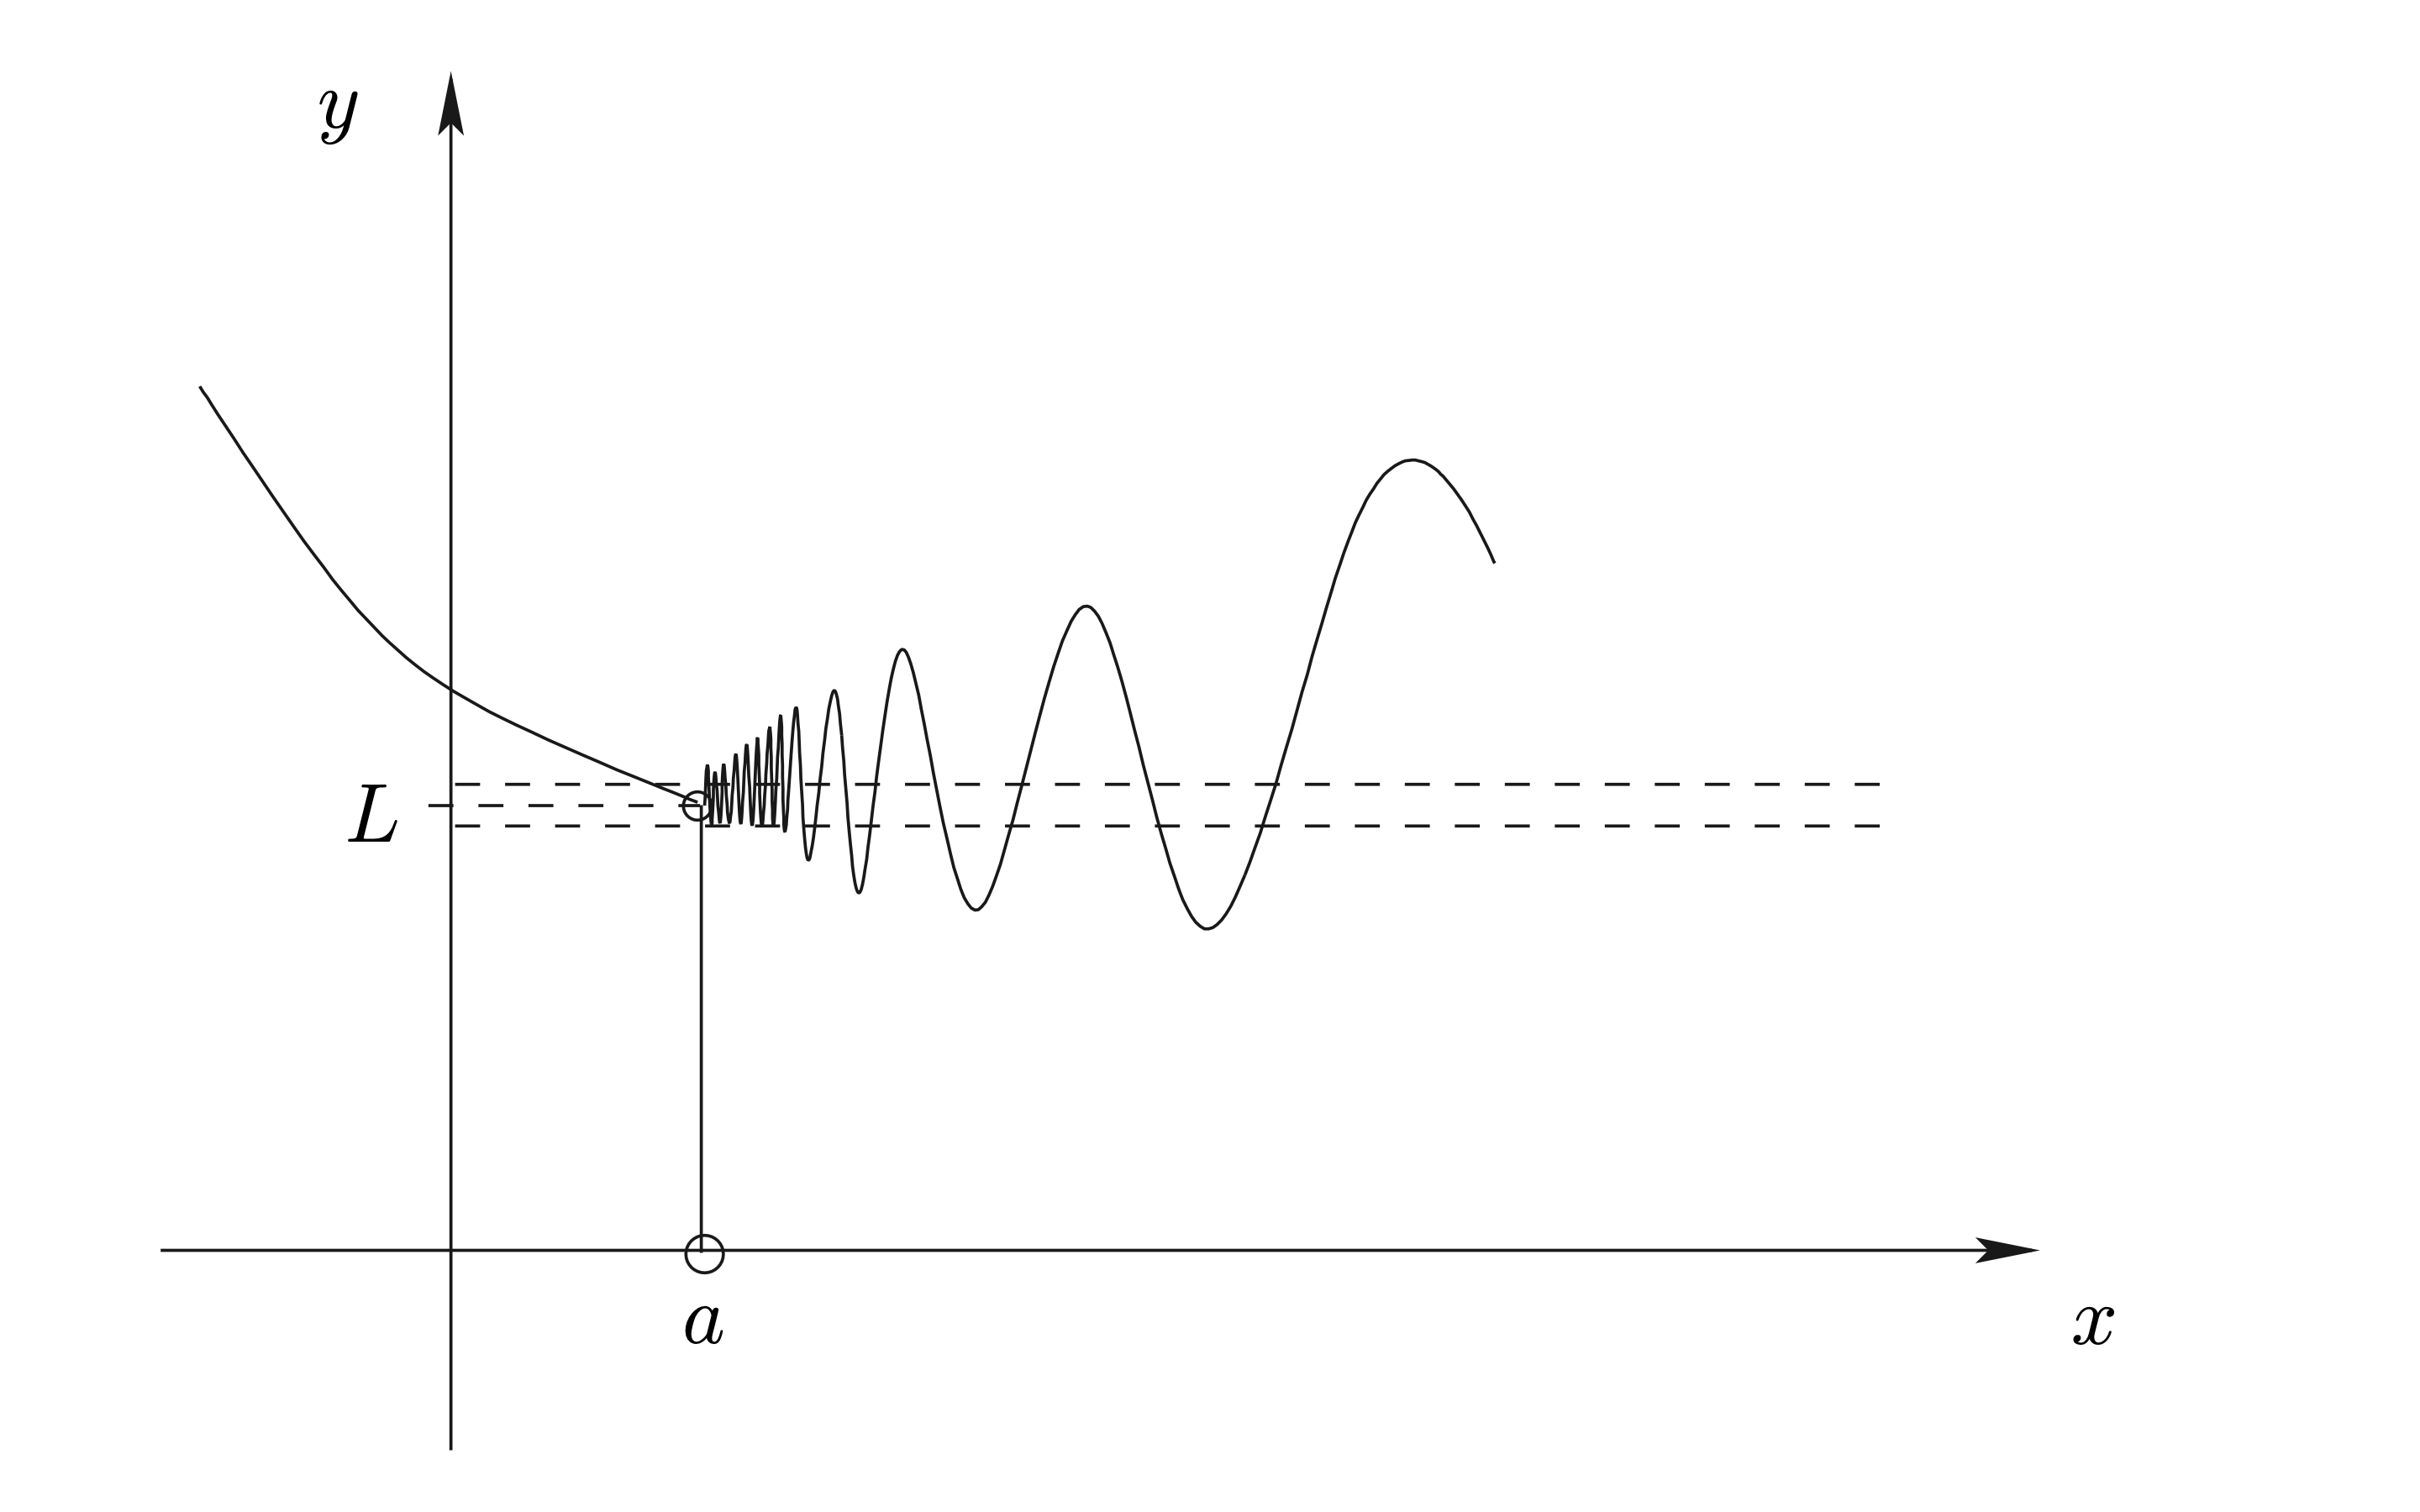
\includegraphics[width=0.5\linewidth]{images/fig-limit-1} 

}

\caption{กราฟของฟังก์ชันที่หาลิมิตไม่ได้}\label{fig:fig-limit-1}
\end{figure}

ในกรณีนี้ จะเห็นว่า ไม่ว่าจะเลือก \(L\) เป็นค่าใด ก็ไม่สามารถสรุปได้ว่า
\(\underset{x\rightarrow 0^{+}}{\lim}f(x)=L\)
เพราะไม่ใช่ทุกครั้งที่เรากำหนดบริเวณรอบ ๆ \(L\) แล้ว function
จะสอดคล้องตามนิยามเสมอไป จึงสรุปว่า \(\underset{x\rightarrow a}{\lim}f(x)=L\)
หาค่าไม่ได้ด้วย

\begin{theorem}
\protect\hypertarget{thm:thm-limit-1}{}\label{thm:thm-limit-1}\leavevmode

\begin{enumerate}
\def\labelenumi{\arabic{enumi}.}
\item
  \(\underset{x\rightarrow c}{\lim}c=c\) ถ้า c เป็นจำนวนจริง
\item
  \(\underset{x\rightarrow a}{\lim}x=a\)
\end{enumerate}

\end{theorem}

\begin{theorem}
\protect\hypertarget{thm:thm-limit-2}{}\label{thm:thm-limit-2}

ถ้า \(\underset{x\rightarrow a}{\lim}f(x)\) และ
\(\underset{x\rightarrow a}{\lim}g(x)\) หาค่าได้แล้ว จะได้

\begin{enumerate}
\def\labelenumi{\arabic{enumi}.}
\item
  \(\underset{x\rightarrow a}{\lim}(f+g)(x)=\underset{x\rightarrow a}{\lim}f(x)+\underset{x\rightarrow a}{\lim}g(x)\)
\item
  \(\underset{x\rightarrow a}{\lim}(f-g)(x)=\underset{x\rightarrow a}{\lim}f(x)-\underset{x\rightarrow a}{\lim}g(x)\)
\item
  \(\underset{x\rightarrow a}{\lim}(f\cdot g)(x)=\left( \underset{x\rightarrow a}{\lim}f(x)\right) \cdot \left( \underset{x\rightarrow a}{\lim}g(x)\right)\)
\item
  \(\underset{x\rightarrow a}{\lim}\left( \frac{f}{g}\right) (x)=\frac{\underset{x\rightarrow a}{\lim}f(x)}{\underset{x\rightarrow a}{\lim}g(x)}\)
  ถ้า \(\underset{x\rightarrow a}{\lim}g(x)\neq 0\)
\end{enumerate}

\end{theorem}

\textbf{หมายเหตุ} ทฤษฎีบททั้งสองนี้ยังคงเป็นจริงสำหรับ limit ทางซ้าย และ limit ทางขวาด้วย

\begin{theorem}
\protect\hypertarget{thm:thm-limit-3}{}\label{thm:thm-limit-3}ถ้า \(\underset{x\rightarrow a}{\lim}f(x)\) หาค่าได้ และ
\(\root{n}\of{f\left( x\right) }\) หาค่าได้ สำหรับทุก ๆ \(x\) ในช่วงเปิดบางช่วงที่มี
\(a\) อยู่ด้วย แล้ว
\(\underset{x\rightarrow a}{\lim}\root{n}\of{f\left( x\right) }=\root{n}\of{\underset{x\rightarrow a}{\lim}f(x)}\)
\end{theorem}

\textbf{หมายเหตุ} ทฤษฎีบทนี้เป็นจริงสำหรับ limit ทางซ้าย และ limit ทางขวาด้วย
โดยเปลี่ยนเงื่อนไข ``ทุก ๆ \(x\)'' เป็น ``ทุก ๆ \(x < a\)'' และ ``ทุก ๆ \(x > a\)'' ตามลำดับ

\begin{theorem}
\protect\hypertarget{thm:thm-limit-4}{}\label{thm:thm-limit-4}ถ้า \(f\) และ \(g\) เป็น function ซึ่ง \(f\left( x\right) =g\left( x\right)\)
สำหรับทุก ๆ \(x\) ยกเว้นบาง \(x\) ซึ่งมีอยู่เพียงจำนวนจำกัด แล้ว
\(\underset{x\rightarrow a}{\lim}f(x)=\underset{x\rightarrow a}{\lim}g(x)\)
ถ้า limit อันใดอันหนึ่งหาค่าได้
\end{theorem}

\textbf{หมายเหตุ} ทฤษฎีบทนี้ยังคงเป็นจริงสำหรับ limit ทางซ้าย และ limit ทางขวาด้วย

\begin{example}
\protect\hypertarget{exm:ex-limit-3}{}\label{exm:ex-limit-3}จงหาค่าของ \(\underset{x\rightarrow 2}{\lim}\frac{-x^{2}+6x-8}{x-2}\)
\end{example}

\textbf{วิธีทำ}

\begin{equation}
  \begin{aligned}
    \lim_{x\rightarrow 2}\frac{-x^{2}+6x-8}{x-2}
    &= \lim_{x\rightarrow 2} -\frac{\left( x-2\right) \left( x-4\right) }{x-2}\\
    &= \lim_{x\rightarrow 2} -\left( x-4\right) \\ %ต่างกับ function เดิม ที่ค่าเดียของ x คือ x = 2
    &= \lim_{x\rightarrow 2}\left( 4-x\right) \\
    &= \lim_{x\rightarrow 2}4-\lim_{x\rightarrow 2}x\\
    &= 4-2 \\
    &= 2
  \end{aligned}
\end{equation}

\begin{example}
\protect\hypertarget{exm:ex-limit-4}{}\label{exm:ex-limit-4}

จงหาค่าของ \(\underset{x\rightarrow 3}{\lim}\frac{\sqrt{x}-\sqrt{3}}{x-3}\)
\textbf{วิธีทำ}

\begin{equation}
  \begin{aligned}
    \lim_{x\rightarrow 3}\frac{\sqrt{x}-\sqrt{3}}{x-3}
    &= \lim_{x\rightarrow 3}\frac{\sqrt{x}-\sqrt{3}}{x-3}\cdot \frac{\sqrt{x}+\sqrt{3}}{\sqrt{x}+\sqrt{3}} \\
    &= \lim_{x\rightarrow 3}\frac{x-3}{\left( x-3\right) \left( \sqrt{x}+\sqrt{3}\right) } \\
    &= \lim_{x\rightarrow 3}\frac{1}{\sqrt{x}+\sqrt{3}}\\
    &= \frac{\lim_{x\rightarrow 3}1}{\lim_{x\rightarrow 3} \sqrt{x} + \lim_{x\rightarrow 3} \sqrt{3}} \\
    &= \frac{\lim_{x\rightarrow 3}1}{\sqrt{\lim_{x\rightarrow 3}x}+\lim_{x\rightarrow 3}\sqrt{3}} \\
    &= \frac{1}{\sqrt{3}+\sqrt{3}} \\
    &= \frac{1}{2\sqrt{3}} \\
  \end{aligned}
\end{equation}

\end{example}

\begin{example}
\protect\hypertarget{exm:ex-limit-5}{}\label{exm:ex-limit-5}

จงหา limits ต่อไปนี้

\begin{enumerate}
\def\labelenumi{\arabic{enumi}.}
\item
  \(\underset{x\rightarrow 0^{+}}{\lim}\frac{\sqrt{x}-\sqrt{3}}{x-3}\)
\item
  \(\underset{x\rightarrow 0^{-}}{\lim}\frac{\sqrt{x}-\sqrt{3}}{x-3}\)
\item
  \(\underset{x\rightarrow 0}{\lim}\frac{\sqrt{x}-\sqrt{3}}{x-3}\)
\end{enumerate}

\end{example}

\textbf{วิธีทำ}

\begin{enumerate}
\def\labelenumi{\arabic{enumi}.}
\item
  \(\underset{x\rightarrow 0^{+}}{\lim}\frac{\sqrt{x}-\sqrt{3}}{x-3}\)\(=\frac{0-\sqrt{3}}{x-3}=\frac{\sqrt{3}}{3}\)
\item
  เนื่องจาก function \(\frac{\sqrt{x}-\sqrt{3}}{x-3}\) ไม่ใช่ function
  ที่หาค่าได้บนช่วงเปิด \(\left( b,0\right)\) ใด ๆ เลย ดังนั้น
  \(\underset{x\rightarrow 0^{-}}{\lim}\frac{\sqrt{x}-\sqrt{3}}{x-3}\)
  จึงหาค่าไม่ได้
\item
  เนื่องจาก
  \(\underset{x\rightarrow 0^{-}}{\lim}\frac{\sqrt{x}-\sqrt{3}}{x-3}\)
  หาค่าไม่ได้ ดังนั้น
  \(\underset{x\rightarrow 0}{\lim}\frac{\sqrt{x}-\sqrt{3}}{x-3}\)
  จึงหาค่าไม่ได้
\end{enumerate}

\textbf{ข้อสังเกต} ในกรณีที่ function ที่มีค่ามากขึ้นโดยไม่มีขอบเขต เมื่อตัวแปรต้นเข้าใกล้ \(a\)
(ทางซ้ายหรือขวา หรือทั้งสองทาง) บางตำรากล่าวว่า limit ของ function มีค่าเป็น
\(+\infty\) และถ้า function มีค่าลดลงโดยไม่มีขอบเขต จะกล่าวว่า limit ของ function
มีค่าเป็น \(-\infty\) ในวิชานี้เราจะถือตามนิยามที่ให้ไว้ ดังนั้นในกรณีข้างต้น จะกล่าวว่า limit
ดังกล่าวหาค่าไม่ได้ (เว้นแต่จะระบุให้พิจารณาค่า \(\pm \infty\) ด้วย)

\begin{example}
\protect\hypertarget{exm:ex-limit-6}{}\label{exm:ex-limit-6}

จงหา limit ของ function \(f\left( x\right) =\frac{1}{x}\)

\begin{enumerate}
\def\labelenumi{\arabic{enumi}.}
\item
  เมื่อ \(x\) เข้าใกล้ 0 ทางซ้าย
\item
  เมื่อ \(x\) เข้าใกล้ 0 ทางขวา
\item
  เมื่อ \(x\) เข้าใกล้ 0
\end{enumerate}

\end{example}

\textbf{วิธีทำ}

\begin{enumerate}
\def\labelenumi{\arabic{enumi}.}
\item
  \(\underset{x\rightarrow 0^{-}}{\lim}\frac{1}{x}\) หาค่าไม่ได้ (หรือเท่ากับ
  \(-\infty\))
\item
  \(\underset{x\rightarrow 0^{+}}{\lim}\frac{1}{x}\) หาค่าไม่ได้ (หรือเท่ากับ
  \(+\infty\))
\item
  \(\underset{x\rightarrow 0}{\lim}\frac{1}{x}\) หาค่าไม่ได้
\end{enumerate}

ในบางครั้ง เราสนใจพฤติกรรมของ function \(f\) เมื่อค่าตัวแปรต้นมีค่ามากขึ้นโดยไม่มีขอบเขต
หรือน้อยลงโดยไม่มีขอบเขต ในกรณีเช่นนี้ เราใช้สัญลักษณ์
\(\underset{x\rightarrow +\infty }{\lim}f\left( x\right)\) และ
\(\underset{x\rightarrow -\infty }{\lim}f\left( x\right)\) ตามลำดับ
แทนที่จะใช้ \(\underset{x\rightarrow \infty ^{-}}{\lim}f\left( x\right)\) และ
\(\underset{x\rightarrow \infty ^{+}}{\lim}f\left( x\right)\)
(โปรดอ่านนิยามในเอกสารอ้างอิง) ทฤษฎีบทเกี่ยวกับ limit ที่กล่าวมาข้างต้นทั้งหมด
เป็นจริงในกรณีนี้ด้ย นอกจากนี้ เรายังมี ทฤษฎีบทต่อไปนี้

\begin{theorem}
\protect\hypertarget{thm:thm-limit-5}{}\label{thm:thm-limit-5}\leavevmode

\begin{enumerate}
\def\labelenumi{\arabic{enumi}.}
\item
  \(\underset{x\rightarrow +\infty }{\lim}x=+\infty\)
\item
  \(\underset{x\rightarrow -\infty }{\lim}x=-\infty\)
\item
  ถ้า \(\underset{x\rightarrow a}{\lim}f\left( x\right) =\pm \infty\) แล้ว
  \(\underset{x\rightarrow a}{\lim}f\left( x\right) =0\) ซึ่งเป็นจริงสำหรับ
  limit ทางซ้าย และ limit ทางขวาด้วย ในที่นี้ \(a\in R\) หรือ a เป็น \(+\infty\)
  หรือ \(-\infty\)
\end{enumerate}

\end{theorem}

\begin{example}
\protect\hypertarget{exm:ex-limit-7}{}\label{exm:ex-limit-7}\(\underset{x\rightarrow -\infty }{\lim}\frac{x^{2}+12}{x^{3}-5}=?\)
\end{example}

\textbf{วิธีทำ}

\begin{equation}
  \begin{aligned}
    \underset{x\rightarrow -\infty }{\lim}\frac{x^{2}+12}{x^{3}-5}
        &=\underset{x\rightarrow -\infty }{\lim}\frac{\left( x^{2}+12\right) /x^{3}}{\left( x^{3}-5\right) /x^{3}} \\
        &=\underset{x\rightarrow -\infty }{\lim}\frac{\frac{1}{x}+\frac{12}{x^{3}}}{1-\frac{5}{x^{3}}}
    =\frac{0+0}{1-0}=0
  \end{aligned}
\end{equation}

\begin{example}
\protect\hypertarget{exm:ex-limit-8}{}\label{exm:ex-limit-8}\(\underset{x\rightarrow +\infty }{\lim}x^{-\frac{2}{3}}=?\)
\end{example}

\textbf{วิธีทำ}

\begin{equation}
  \begin{aligned}
    \underset{x\rightarrow +\infty }{\lim}x^{-\frac{2}{3}}
        &=\underset{x\rightarrow +\infty }{\lim}\root{3}\of{\left( \frac{1}{x}\right) ^{2}} \\
        &=\root{3}\of{\left( \underset{x\rightarrow +\infty }{\lim}\frac{1}{x}\right) ^{2}}
            =0
  \end{aligned}
\end{equation}

\begin{example}
\protect\hypertarget{exm:ex-limit-9}{}\label{exm:ex-limit-9}\(\underset{x\rightarrow +\infty }{\lim}\frac{x^{\frac{1}{3}}+3x^{\frac{1}{5}}+5x^{\frac{1}{7}}}{3x^{\frac{1}{3}}+5x^{\frac{1}{5}}+7x^{\frac{1}{7}}}=?\)
\end{example}

\textbf{วิธีทำ}

\begin{equation}
  \begin{aligned}
    \underset{x\rightarrow +\infty }{\lim}\frac{x^{\frac{1}{3}}+3x^{\frac{1}{5}}+5x^{\frac{1}{7}}}{3x^{\frac{1}{3}}+5x^{\frac{1}{5}}+7x^{\frac{1}{7}}}
        &=\underset{x\rightarrow +\infty }{\lim}\frac{x^{\frac{1}{3}}\left( 1+3x^{-\frac{2}{15}}+5x^{-\frac{4}{21}}\right) }{x^{\frac{1}{3}}\left( 3+5x^{-\frac{2}{15}}+7x^{-\frac{4}{21}}\right) } \\
        &=\underset{x\rightarrow +\infty }{\lim}\frac{1+3x^{-\frac{2}{15}}+5x^{-\frac{4}{21}}}{3+5x^{-\frac{2}{15}}+7x^{-\frac{4}{21}}}
=\frac{1}{3}
  \end{aligned}
\end{equation}

\textbf{ข้อสังเกต} ตัวแปร \(x\) ในสัญลักษณ์
\(\underset{x\rightarrow a}{\lim}f\left( x\right)\) เรียกว่า ``ตัวแปรหุ่น''
(dummy variable) เพราะไม่ได้กล่าวถึงตัวแปร \(x\)
แต่เราใช้มันเพื่อเขียนสัญลักษณ์แทนจำนวนจริงจำนวนหนึ่งที่ค่าของ function \(f\) ใกล้เข้าไปหา
ในยามที่ตัวแปรต้นของมันมีค่าใกล้ \(a\) เข้าไปทุกที เราอาจเขียน
\(\underset{t\rightarrow a}{\lim}f\left( t\right)\) แทนจำนวนจำนวนนี้ก็ได้
เป็นต้น ตัวอย่างของ dummy variable อื่น ๆ เช่น ตัวแปร \(n\) ในสัญลักษณ์
\(\underset{n=1}{\overset{4}{\sum }}n^{2}\) ซึ่งอาจเขียนใหม่เป็น
\(\underset{k=1}{\overset{4}{\sum }}k^{2}\) ก็ได้ ทั้งสองสัญลักษณ์นี้แทนจำนวน
\(1^{2}+2^{2}+3^{3}+4^{4}\)

\begin{example}
\protect\hypertarget{exm:ex-limit-10}{}\label{exm:ex-limit-10}จงหา \(\underset{x\rightarrow 3}{\lim}f\left( x\right)\) เมื่อ

\[
f(x) =
\begin{cases}
x^2 - 5 & \text{ถ้า } x \leq 3 \\
\sqrt{x + 13} & \text{ถ้า } x > 3
\end{cases}
\]
\end{example}

\textbf{วิธีทำ}

\begin{equation}
  \begin{aligned}
    \underset{x\rightarrow 3^{-}}{\lim}f\left( x\right)
    &=\underset{x\rightarrow 3^{-}}{\lim}x^{2}-5 \leftarrow \boxed{  f(x) = x^{2}-5  \mbox{ เมื่อ $x$ อยู่ทางซ้ายของ 3}}\\
    &=4
  \end{aligned}
\end{equation}

\begin{equation}
  \begin{aligned}
    \underset{x\rightarrow 3^{+}}{\lim}f\left( x\right)
        &= \underset{x\rightarrow 3^{+}}{\lim}\sqrt{x+13} \leftarrow
        \boxed{ f(x)=\sqrt{x+13} \mbox{ เมื่อ $x$ อยู่ทางขวาของ 3}} \\
        &=4
  \end{aligned}
\end{equation}

เนื่องจาก
\(\underset{x\rightarrow 3^{-}}{\lim}f\left( x\right) =\)~\(\underset{x\rightarrow 3^{+}}{\lim}f\left( x\right) =4\)
ดังนั้น ~\(\underset{x\rightarrow 3}{\lim}f\left( x\right)\) หาค่าได้
และมีค่าเท่ากับ 4

\begin{example}
\protect\hypertarget{exm:ex-limit-11}{}\label{exm:ex-limit-11}จงหา \(\underset{x\rightarrow 0}{\lim}f\left( x\right)\) เมื่อ
\[f(x) = \begin{cases}
            x^{2}-5 & \text{ ถ้า } x\leq 3 \\
            \sqrt{x+13}  & \text{ ถ้า } x>3
              \end{cases}\]
\end{example}

\textbf{วิธีทำ}
\(\underset{x\rightarrow 0}{\lim}f(x)=\underset{x\rightarrow 0}{\lim}(x^{2}-5)=-5\)

\section{ความต่อเนื่อง (Continuity)}\label{uxe04uxe27uxe32uxe21uxe15uxe2duxe40uxe19uxe2duxe07-continuity}

ในวิชาฟิสิกส์ เราสามารถเขียนตำแหน่งของวัตถุที่กำลังเคลื่อนที่ในรูป function ของเวลาได้
(วัตถุย่อมอยู่ในที่ใดที่หนึ่งเพียงที่เดียว ณ เวลาหนึ่ง ๆ)

\textbf{คำถาม} : function ใด ๆ เป็น function
ที่แสดงตำแหน่งของวัตถุใดวัตถุหนึ่งได้เสมอหรือไม่

ลองอธิบายการเคลื่อนที่ของวัตถุ ถ้า function ที่แสดงตำแหน่งของมัน คือ

\begin{enumerate}
\def\labelenumi{\arabic{enumi}.}
\item
  \(s_{1}(t)  = \begin{cases}
              1 & \text{ ถ้า } t<3 \\
              1  & \text{ ถ้า } t>3
                \end{cases}\)
\item
  \(s_{2}(t)  = \begin{cases}
              0 & \text{ ถ้า } t \le 3 \\
              1  & \text{ ถ้า } t>3
                \end{cases}\)
\item
  \(s_{3}(t)  = \begin{cases}
              1 & \text{ ถ้า } t \neq 3 \\
              0  & \text{ ถ้า } t=3
                \end{cases}\)
\end{enumerate}

กราฟของ \(s_1,s_2\) และ \(s_3\) เป็นดังนี้

\textbf{ข้อสังเกต}:

\begin{enumerate}
\def\labelenumi{\arabic{enumi}.}
\item
  \(s_1(3)\) หาค่าไม่ได้
\item
  \(s_2(3)\) หาค่าได้ แต่ \(\underset{t \rightarrow 3}{\lim} s_2(t)\)
  หาค่าไม่ได้
\item
  \(s_3(3)\) หาค่าได้ \(\underset{t \rightarrow 3}{\lim} s_3(t)\) หาค่าได้ แต่
  \(s_3(3) \neq \underset{t \rightarrow 3}{\lim} s_3(t)\)
\end{enumerate}

\begin{figure}

{\centering 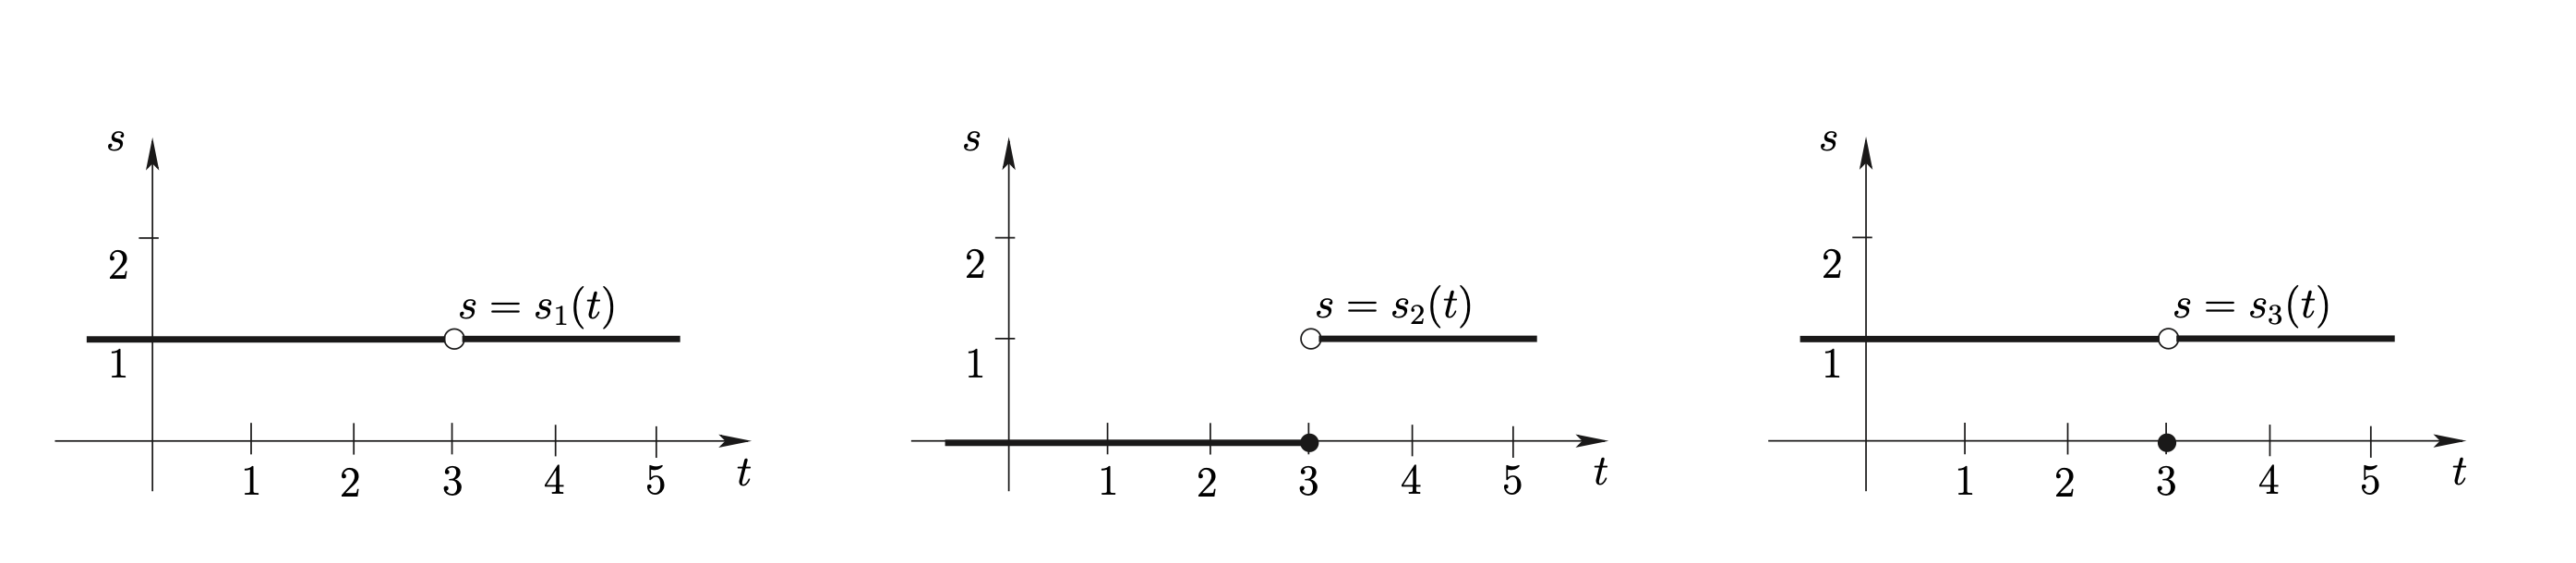
\includegraphics[width=0.5\linewidth]{images/fig-continuity-1} 

}

\caption{กราฟของฟังก์ชัน $s_1$, $s_2$ และ $s_3$}\label{fig:fig-continuity-1}
\end{figure}

\begin{definition}

ให้ \(f:D_{f}\rightarrow R\) โดยที่ \(D_{f}\subseteq R\) และ \(a\in R\) เรากล่าวว่า
\(f\) ต่อเนื่อง (cotinuous) ที่ \(a\) ถ้า

\begin{enumerate}
\def\labelenumi{\arabic{enumi}.}
\item
  \(f \left( a\right)\) หาค่าได้
\item
  \(\underset{x\rightarrow a}{\lim}f(x)\) หาค่าได้
\item
  \(f\left( a\right) =\underset{x\rightarrow a}{\lim}f(x)\)
\end{enumerate}

\end{definition}

\begin{definition}
ให้ \(f\) เป็น function และ \(S\) เป็นเซต (set) เรากล่าวว่า \(f\) ต่อเนื่องบน \(S\)
(continuous on \(S\)) ถ้า \(f\) ต่อเนื่องที่ทุก ๆ สมาชิกของ \(S\) เรียก function ที่
continuous on \(R\) ว่า ``ฟังก์ชันต่อเนื่อง (continuous function)''
\end{definition}

\textbf{ข้อสังเกต} จะเห็นว่า function ที่แสดงตำแหน่งของวัตถุต้องเป็น continuous function
บนช่วงที่สนใจ

\begin{theorem}
\protect\hypertarget{thm:thm-cont-1}{}\label{thm:thm-cont-1}

ถ้า \(f\) และ \(g\) เป็น function ที่ต่อเนื่องที่ \(a\) แล้ว

\begin{enumerate}
\def\labelenumi{\arabic{enumi}.}
\item
  \(f+g\) ต่อเนื่องที่ \(a\)
\item
  \(f-g\) ต่อเนื่องที่ \(a\)
\item
  \(f\cdot g\) ต่อเนื่องที่ \(a\)
\item
  \(\frac{f}{g}\) ต่อเนื่องที่ \(a\) ถ้า \(g\left( a\right) \neq 0\)
\end{enumerate}

\end{theorem}

\begin{example}
\protect\hypertarget{exm:ex-cont-1}{}\label{exm:ex-cont-1}function \(f\) ซึ่งนิยามโดย \(f\left( x\right) =\left| x\right|\)
เป็นฟังก์ชันต่อเนื่องหรือไม่
\end{example}

\textbf{วิธีทำ} ในที่นี้ \[f\left( x\right) =
             \begin{cases}
            x & \text{ ถ้า } x \ge 0 \\
            -x  & \text{ ถ้า } x>0
              \end{cases}\] เราต้องพิจารณาว่า \(f\) ต่อเนื่องที่ทุก ๆ \(a\in R\)
หรือไม่

\begin{itemize}
\item
  ถ้า \(a>0\) จะได้
  \(\underset{x\rightarrow a}{\lim}f(x)=\underset{x\rightarrow a}{\lim}x=a=f(a)\)
\item
  ถ้า \(a<0\) จะได้
  \(\underset{x\rightarrow a}{\lim}f(x)=\underset{x\rightarrow a}{\lim}(-x)=-a=f(a)\)
\item
  ถ้า \(a=0\)จะได้
  \(\underset{x\rightarrow 0^{-}}{\lim}f(x)=\underset{x\rightarrow 0^{-}}{\lim}(-x)=0=f(0)\)\\
  และ
  \(\underset{x\rightarrow 0^{+}}{\lim}f(x)=\underset{x\rightarrow 0^{+}}{\lim}x=0=f(0)\)\\
  ดังนั้น \(\underset{x\rightarrow 0}{\lim}f(x)=0=f(0)\)
\end{itemize}

ดังนั้น \(f\) ต่อเนื่องที่ทุก ๆ \(a\in R\) จึงสรุปว่า \(f\) เป็น continuous function

\begin{theorem}
\protect\hypertarget{thm:thm-cont-2}{}\label{thm:thm-cont-2}ฟังก์ชันตรรกยะ (rational function) เป็น function ที่ต่อเนื่องบน domain ของมัน
\end{theorem}

\textbf{หมายเหตุ}: rational function คือ function ที่เป็นเศษส่วนของพหุนาม
(polynomial) domain ของ rational function
ได้แก่เซตของจำนวนจริงซึ่งไม่ทำให้ส่วนของมันเป็นศูนย์

\begin{theorem}
\protect\hypertarget{thm:thm-cont-3}{}\label{thm:thm-cont-3}ถ้า \(f\) และ \(g\) เป็น function และ \(a\in R\) โดยที่
\(\underset{x\rightarrow a}{\lim}g(x)=L\) และ \(f\) ต่อเนื่องที่ \(L\) แล้ว
\(\underset{x\rightarrow a}{\lim}f(g(x))=f(\underset{x\rightarrow a}{\lim}g(x))=f(L)\)
\end{theorem}

\begin{example}
\protect\hypertarget{exm:ex-cont-2}{}\label{exm:ex-cont-2}\(\underset{x\rightarrow 1}{\lim}\left| \frac{x^{4}-x^{2}+1}{x^{4}+x^{2}+1}\right| =?\)
\end{example}

\textbf{วิธีทำ}

\begin{equation}
  \begin{aligned}
    \underset{x\rightarrow 1}{\lim}\left| \frac{x^{4}-x^{2}+1}{x^{4}+x^{2}+1}\right|
    &=\left| \ \underset{x\rightarrow 1}{\lim}\frac{x^{4}-x^{2}+1}{x^{4}+x^{2}+1}\right| \\
    &=\left| \frac{1^{4}-1^{2}+1}{1^{4}+1^{2}+1}\right| \\
    &=\left| \frac{1}{3}\right| =\frac{1}{3}
  \end{aligned}
\end{equation}

\begin{theorem}
\protect\hypertarget{thm:thm-cont-4}{}\label{thm:thm-cont-4}ถ้า \(f\) ต่อเนื่องที่ \(a\) และ \(g\) ต่อเนื่องที่ \(f(a)\) แล้ว \(g\circ f\) ต่อเนื่องที่ \(a\)
\end{theorem}

\textbf{จงพิสูจน์ทฤษฎีบทข้างต้น}

\begin{example}
\protect\hypertarget{exm:ex-cont-3}{}\label{exm:ex-cont-3}function f ซึ่งนิยามโดย
\(\ f\left( x\right) =\left| \frac{x^{4}-x^{2}+1}{x^{4}+x^{2}+1}\right|\)
เป็น continuous function หรือไม่
\end{example}

\textbf{วิธีทำ} \(f\) เป็น continuous function เพราะ \(f =g\circ h\) โดยที่
\(g\left( x\right) =\left| x\right|\) และ
\(h\left( x\right) =\frac{x^{4}-x^{2}+1}{x^{4}+x^{2}+1}\) ซึ่งเป็น continuous
function ทั้งคู่

\begin{definition}

เรานิยาม ``ภาวะต่อเนื่องทางซ้าย'' และ ``ภาวะต่อเนื่องทางขวา'' ได้โดยแทนที่
\(\underset{x\rightarrow a}{\lim}\) ในเงื่อนไขของนิยาม ด้วย
\(\underset{x\rightarrow a^{-}}{\lim}\) และ
\(\underset{x\rightarrow a^{+}}{\lim}\) ตามลำดับ นั่นคือ

ให้ \(f:D_{f}\rightarrow R\) โดยที่ \(D_{f}\subseteq R\) และ \(a\in R\) เรากล่าวว่า
\(f\) ``ต่อเนื่องทางซ้าย (left-continuous) ที่ \(a\)'' ถ้า

\begin{enumerate}
\def\labelenumi{\arabic{enumi}.}
\item
  \(f\left( a\right)\) หาค่าได้
\item
  \(\underset{x\rightarrow a^{-}}{\lim}f(x)\) หาค่าได้
\item
  \(f\left( a\right) =\underset{x\rightarrow a^{-}}{\lim}f(x)\)
\end{enumerate}

และกล่าวว่า \(f\) ``ต่อเนื่องทางขวา (right-continuous) ที่ \(a\)'' ถ้า

\begin{enumerate}
\def\labelenumi{\arabic{enumi}.}
\item
  f\(\left( a\right)\) หาค่าได้
\item
  \(\underset{x\rightarrow a^{+}}{\lim}f(x)\) หาค่าได้
\item
  f\(\left( a\right) =\underset{x\rightarrow a^{+}}{\lim}f(x)\)
\end{enumerate}

\end{definition}

\begin{definition}

ให้ \(f : \left[ a,b\right] \rightarrow R\) เรากล่าวว่า \(f\) ต่อเนื่องบน
\(\left[ a,b\right]\) (continuous on \(\left[ a,b\right]\)) ถ้า

\begin{enumerate}
\def\labelenumi{\arabic{enumi}.}
\item
  \(f\) ต่อเนื่องบน \((a,b)\)
\item
  \(f\) ต่อเนื่องทางขวาที่ \(a\)
\item
  \(f\) ต่อเนื่องทางซ้ายที่ \(b\)
\end{enumerate}

\end{definition}

\begin{example}
\protect\hypertarget{exm:ex-cont-4}{}\label{exm:ex-cont-4}function \(f\) ที่นิยามโดย \(f\left( x\right) =\sqrt{4-x^{2}}\) เป็น continuous
function บน \(\left[ -2,2\right]\) หรือไม่
\end{example}

\textbf{วิธีทำ} เราตรวจสอบได้ว่า \(f\) เป็น continuous function บน
\(\left[ -2,2\right]\) เพราะ\\
1. \(f\) เป็น continuous function บน \(\left( -2,2\right)\)\\
2. \(f\) ต่อเนื่องทางขวาที่ -2 เพราะ \$\$

\begin{equation}
  \begin{aligned}
    \underset{x\rightarrow -2^{+}}{\lim}f(x)
        &=\underset{x\rightarrow -2^{+}}{\lim}\sqrt{4-x^{2}} \\
        &=0=f\left( -2\right)
  \end{aligned}
\end{equation}

\begin{enumerate}
\def\labelenumi{\arabic{enumi}.}
\setcounter{enumi}{2}
\tightlist
\item
  \(f\) ต่อเนื่องทางซ้าย ที่ 2 เพราะ
\end{enumerate}

\begin{equation}
  \begin{aligned}
        \underset{x\rightarrow -2^{-}}{\lim}f(x)
        &=\underset{x\rightarrow -2^{-}}{\lim}\sqrt{4-x^{2}} \\
        &=0 =f\left( 2\right)
  \end{aligned}
\end{equation}

\begin{example}
\protect\hypertarget{exm:ex-cont-5}{}\label{exm:ex-cont-5}

พิจารณา function f ซึ่งมีกราฟดังต่อไปนี้

\begin{figure}

{\centering 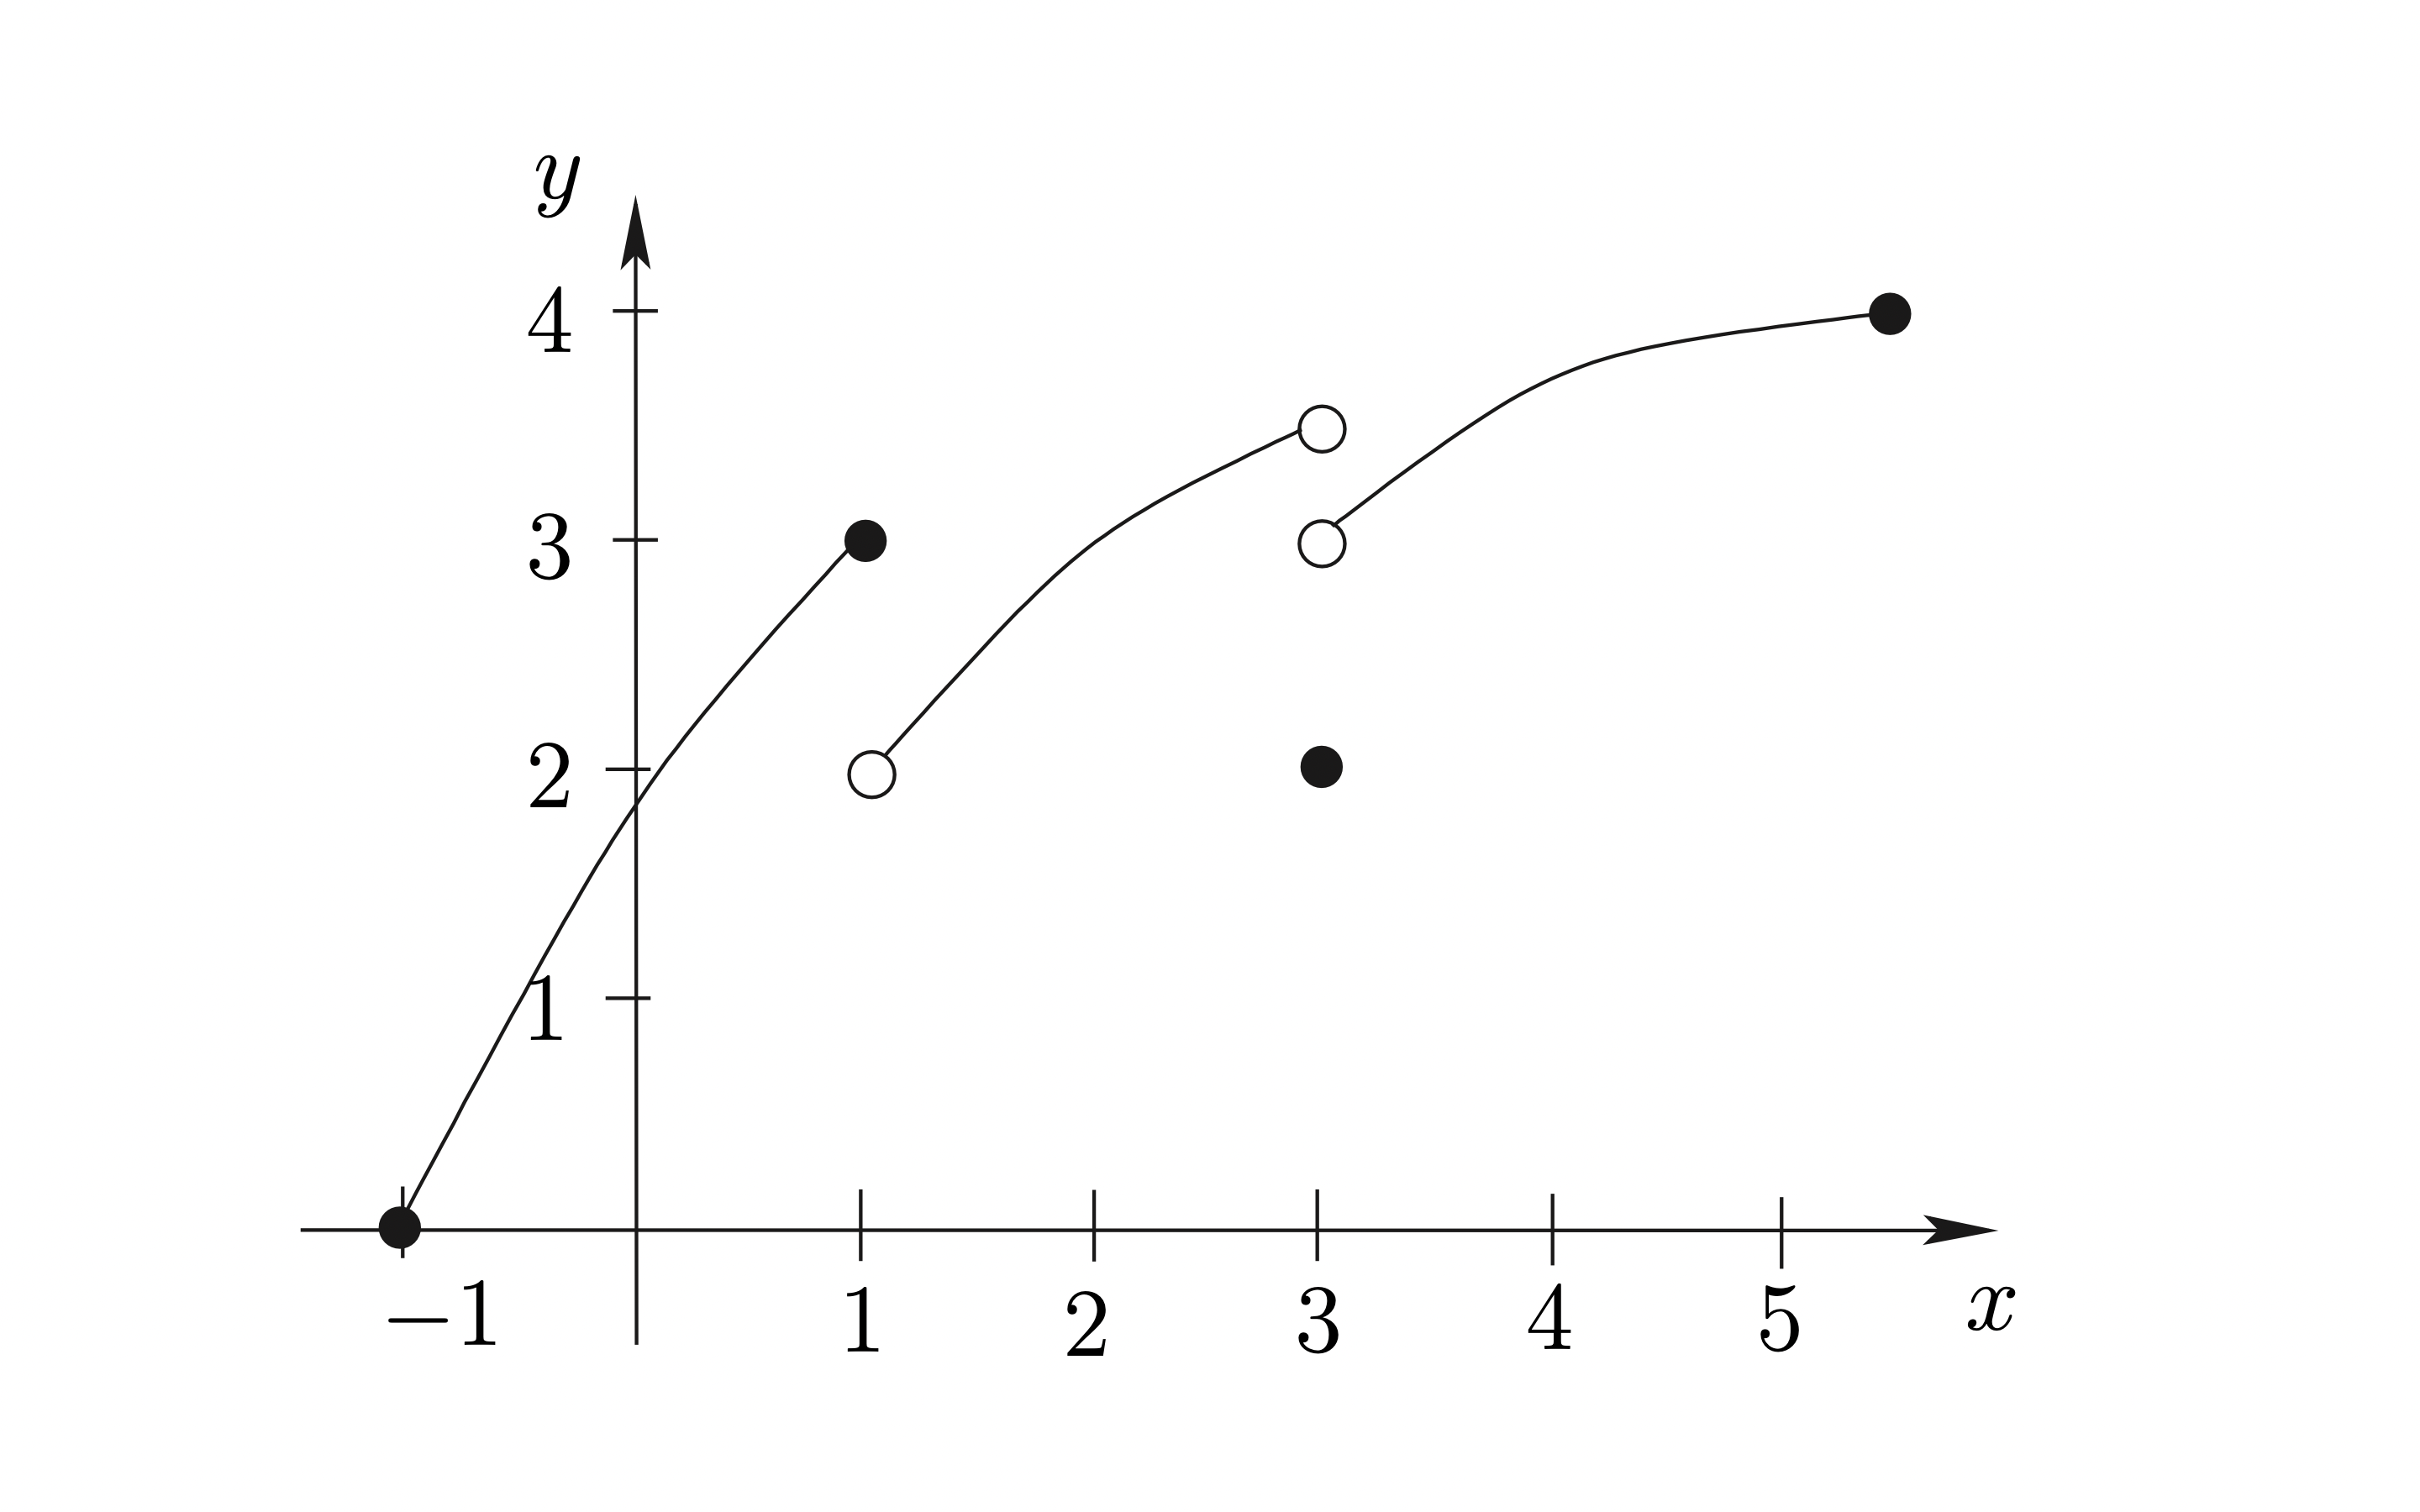
\includegraphics[width=0.5\linewidth]{images/fig-continuity-2} 

}

\caption{กราฟของฟังก์ชันในตัวอย่าง \\ref{exm:ex-cont-5}}\label{fig:fig-continuity-2}
\end{figure}

\begin{enumerate}
\def\labelenumi{\arabic{enumi}.}
\tightlist
\item
  \(f\) มีความต่อเนื่องที่ \(-1,0,1,2,3,4,5\) หรือไม่\\
\item
  \(f\) มีความต่อเนื่องบน
  \(\left[ -1,0\right] ,\left[ 0,1\right] ,\left[ 1,2\right] ,\left[ 2,3\right] ,\left[ 3,4\right] ,\left[ 4,5\right]\)
  หรือไม่
\end{enumerate}

\end{example}

\textbf{วิธีทำ} ให้นักศึกษาทำเป็นแบบฝึกหัด

\begin{theorem}
\protect\hypertarget{thm:thm-cont-5}{}\label{thm:thm-cont-5}ฟังก์ชันตรีโกณมิติ ฟังก์ชันตรีโกณมิติผกผัน ฟังก์ชันเลขชี้กำลัง และฟังก์ชันลอการิทึม
เป็นฟังก์ชันที่ต่อเนื่องบนโดเมนของมัน
\end{theorem}

\chapter{อนุพันธ์ (Derivatives)}\label{uxe2duxe19uxe1euxe19uxe18-derivatives}

\section{อนุพันธ์ (Derivatives)}\label{uxe2duxe19uxe1euxe19uxe18-derivatives-1}

จากตัวอย่า 2.1 ในบทที่ 2 และเนื้อหาในเรื่อง limits เราจะเห็นว่า
ความชันของเส้นสัมผัสกราฟของฟังก์ชัน \(y=f\left( x\right)\) ณ จุด
\(\left( x_{0},f\left( x_{0}\right) \right)\) บนกราฟ ก็คือ
\(\underset{x\rightarrow x_{0}}{\lim}\frac{f\left( x\right) -f\left( x_{0}\right) }{x-x_{0}}\)
นั่นเอง (ถ้า limit หาค่าได้)

\begin{figure}

{\centering 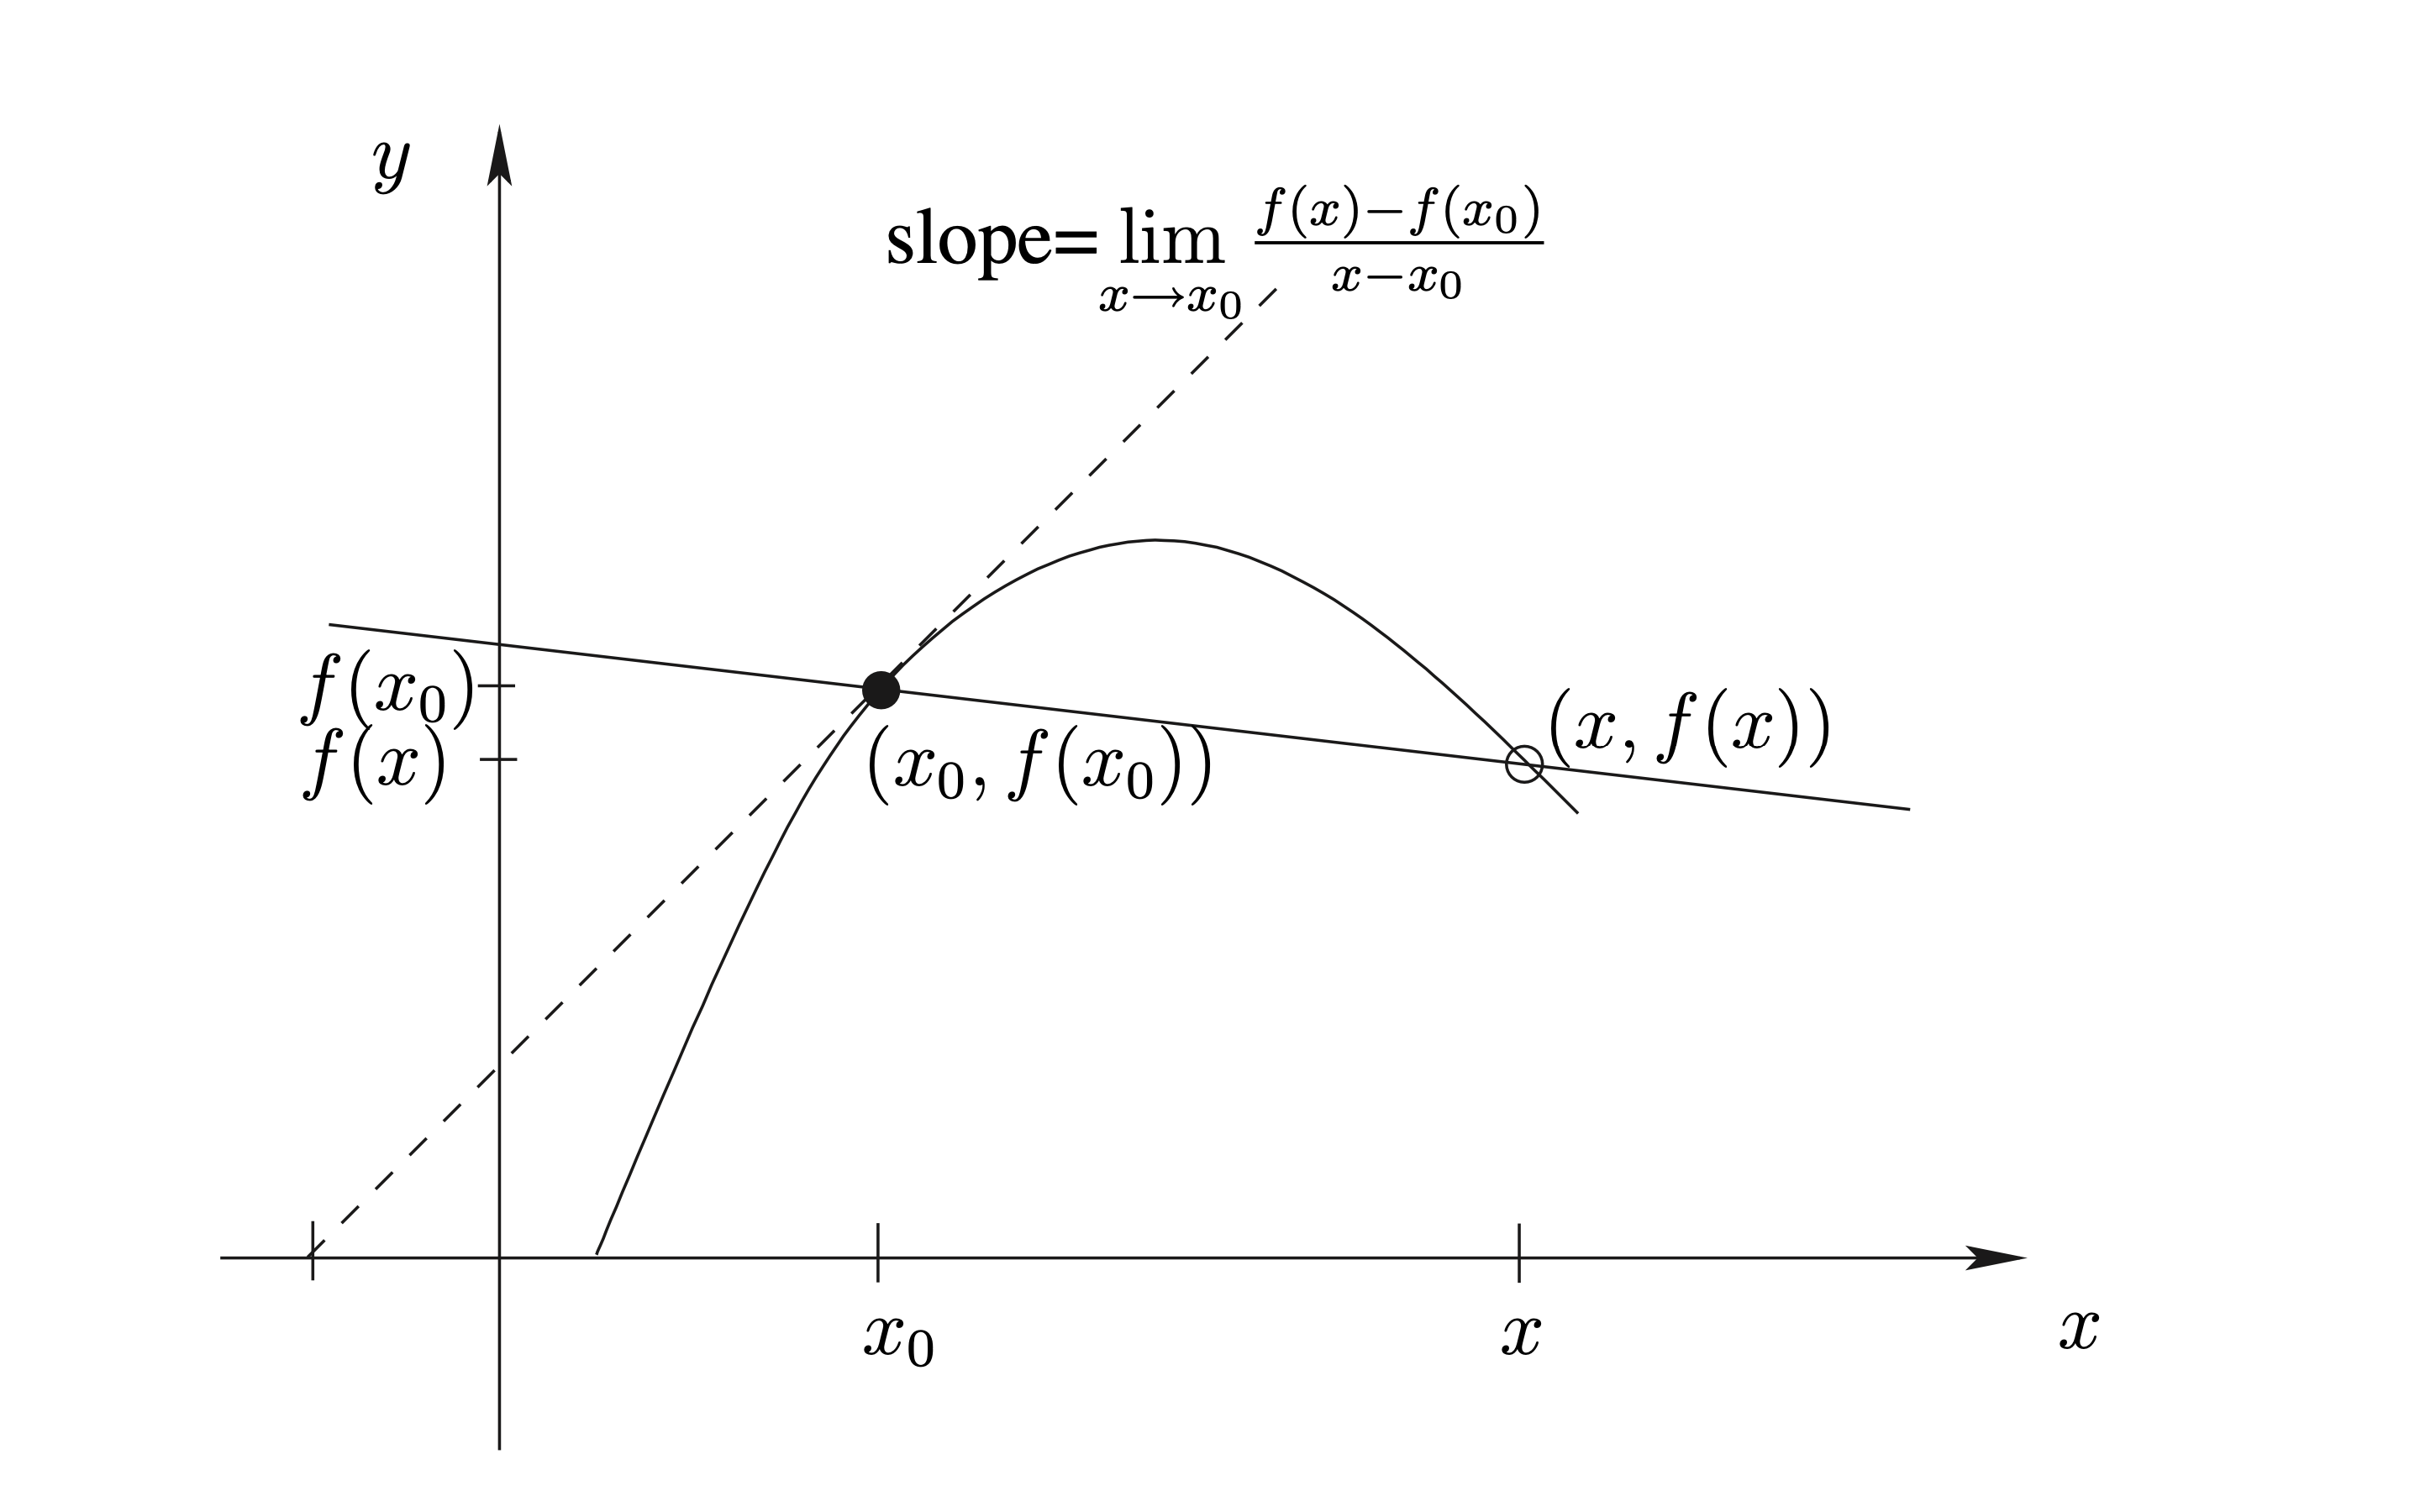
\includegraphics[width=0.5\linewidth]{images/fig-derivative-1} 

}

\end{figure}

ปริมาณนี้มีความสำคัญ เพราะนำไปประยุกต์ใช้ได้มากมาย
เราจึงกำหนดสัญลักษณ์และมีชื่อเรียกดังต่อไปนี้

\begin{definition}
ถ้า \(f : D_f \rightarrow \mathbb{R}\) โดยที่ \(D_f \subseteq \mathbb{R}\)
และถ้า \(\underset{x \rightarrow x_0}{\lim} \frac{f(x)-f(x_0)}{x- x_0}\)
หาค่าได้แล้ว เรียกค่าของ limit นี้ว่า ``อนุพันธ์ (derivative) ของ \(f\) ที่ \(x_0\)''
และแทนด้วยสัญลักษณ์ \(f'(x_0)\)
\end{definition}

เนื่องจากแต่ละ function \(g\) และแต่ละ \(x_0\) จะมี
\(\underset{x \rightarrow x_0}{\lim}g(x)\) ได้ค่าเดียว ดังนั้น \(f'\) จึงเป็น
function เรียกว่า ``อนุพันธ์ (derivative)'' ของ \(f\)

ในการเขียนนิยามของ \(f'(x)\) เพื่อใช้เป็นสูตรทั่วไปสำหรับ function \(f'\)
เราเปลี่ยนตัวแปรเสียใหม่ ดังแสดงในรูป

\begin{figure}

{\centering 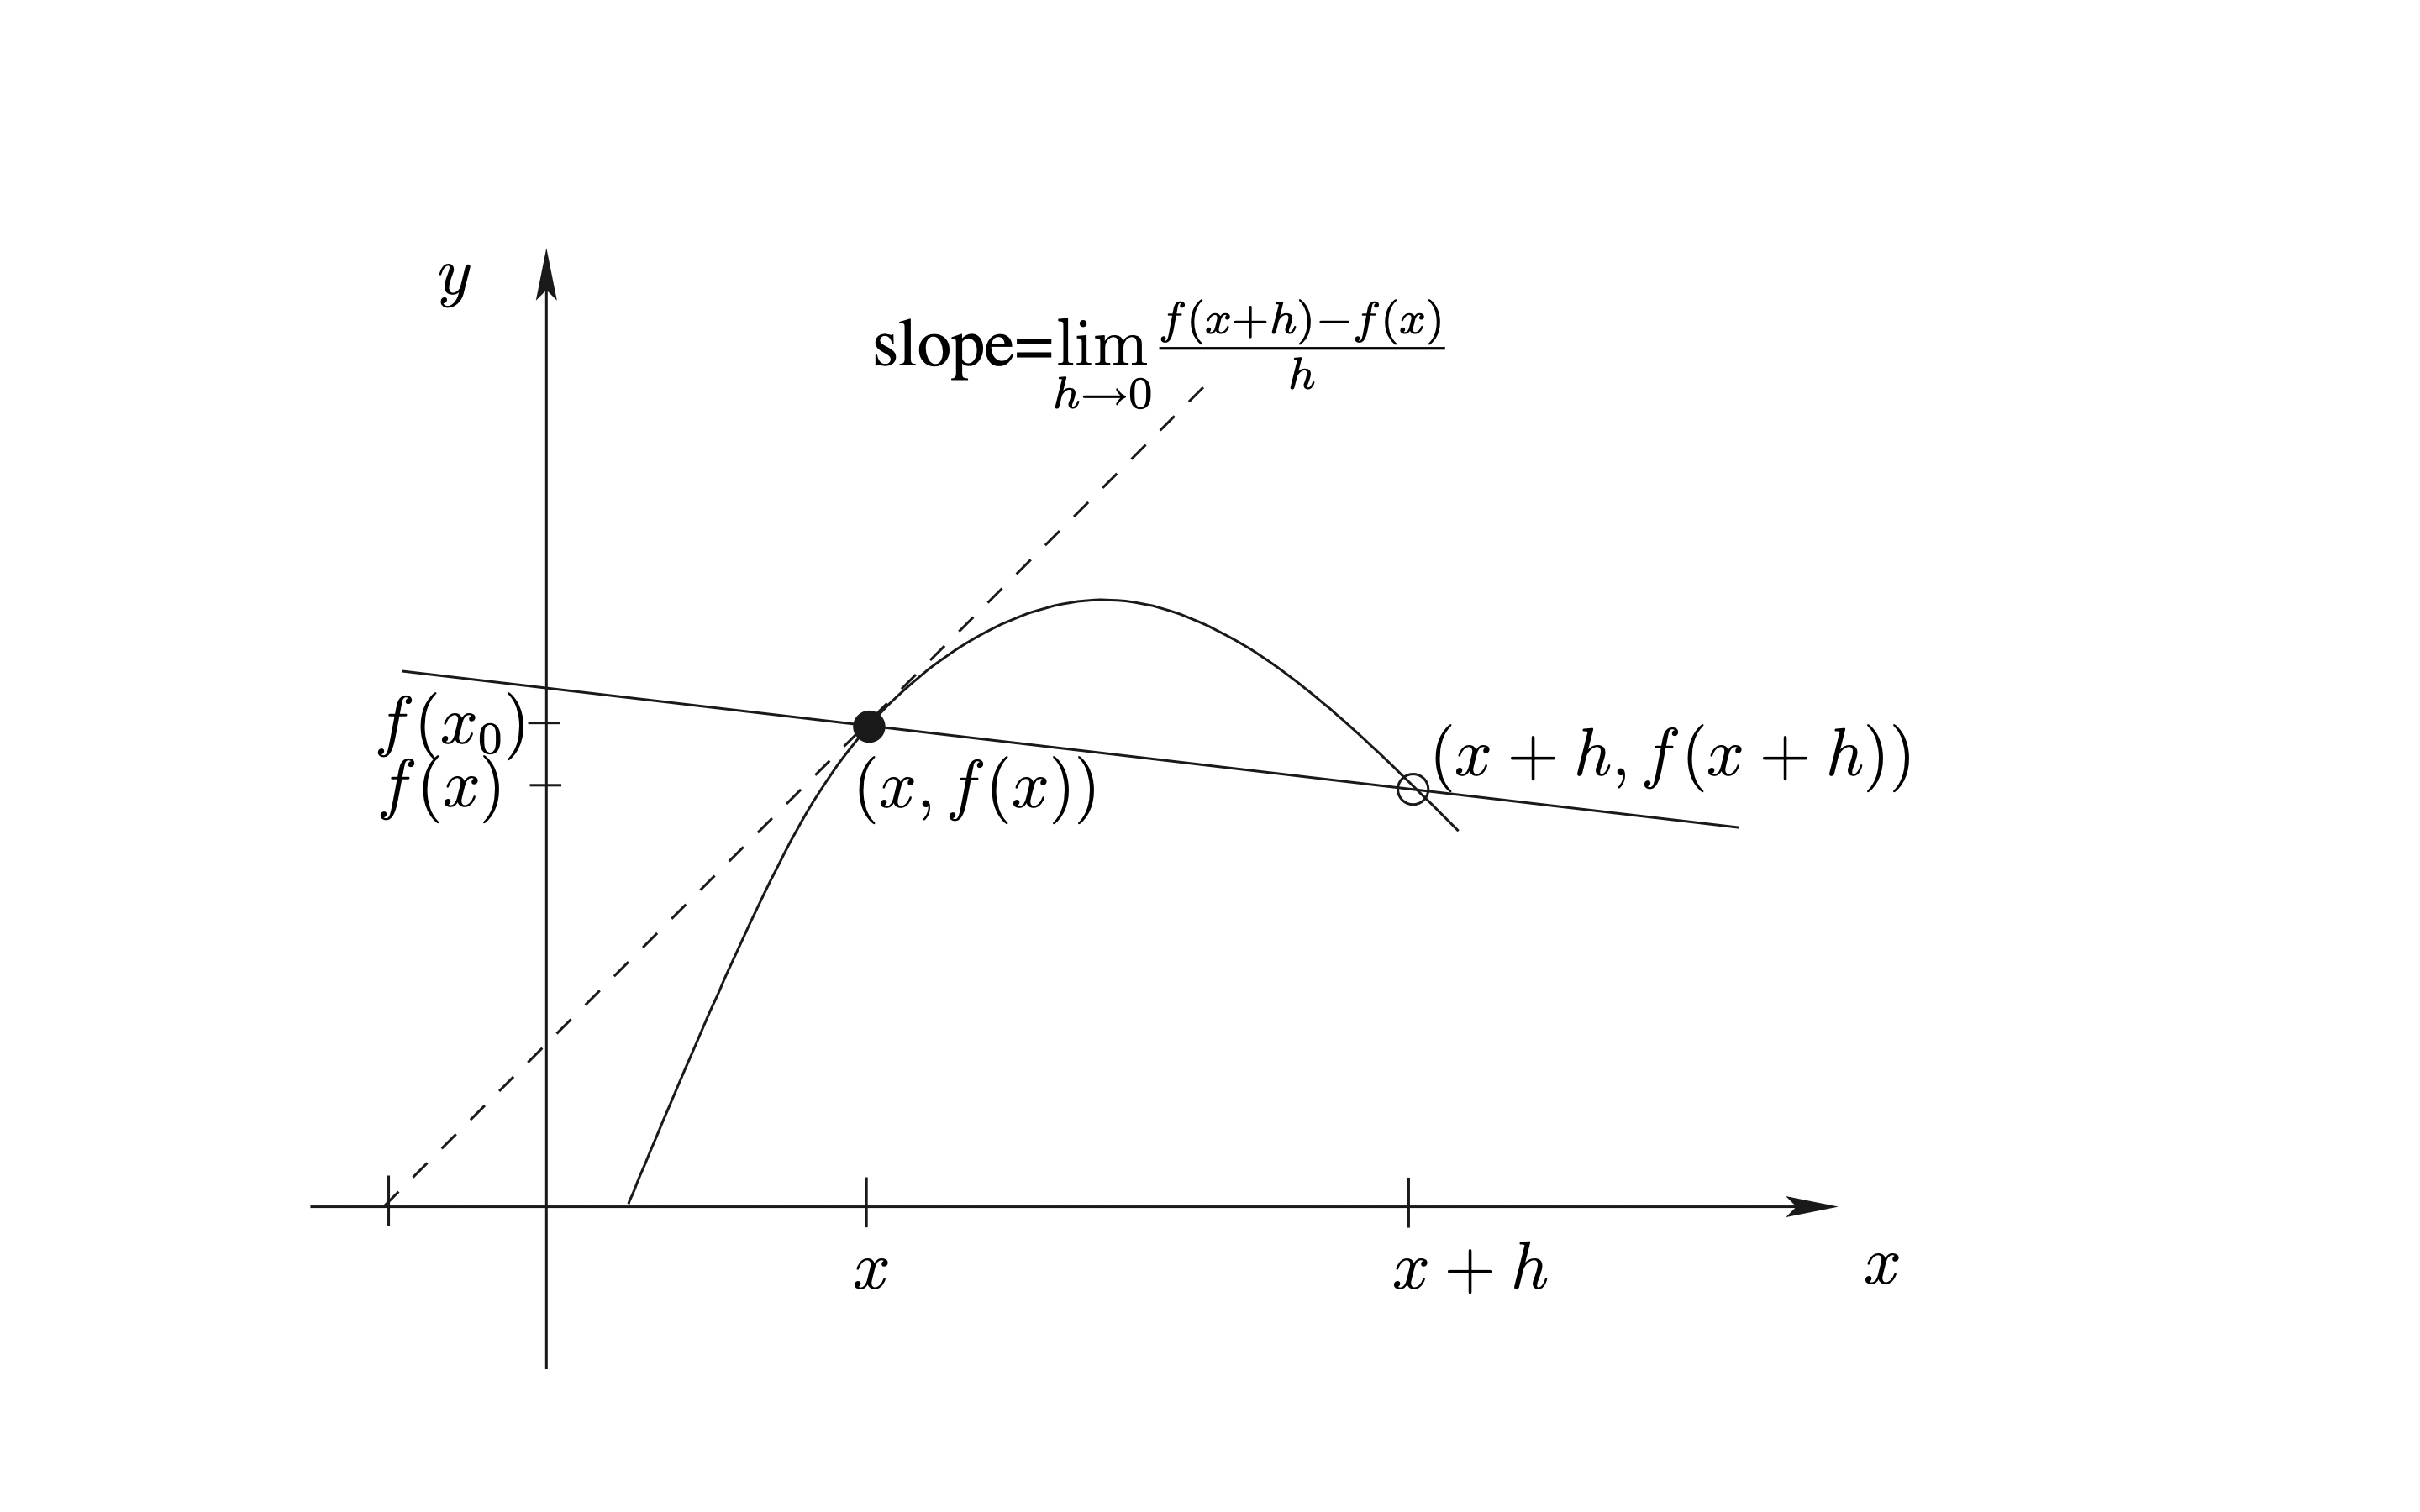
\includegraphics[width=0.5\linewidth]{images/fig-derivative-2} 

}

\end{figure}

จะได้ว่า

\begin{example}
จงหาสมการของเส้นสัมผัสกราฟ \(y = -x^2 + 6x -2\) ณ จุด \(P_0(2,6)\)
\end{example}

\textbf{วิธีทำ} ให้ \(f(x) = -x^2 + 6x -2\) จะได้ค่าความชันของเส้นสัมผัส ณ จุด \((x,f(x))\)
คือ \(f'(x)\) ซึ่งเท่ากับ \begin{equation}   \begin{aligned}
    \underset{h \rightarrow 0}{\lim}\frac{f(x+h) - f(x)}{h}
        &= \underset{h \rightarrow 0}{\lim}\frac{\left[-(x+h)^2 + 6(x+h)-2 \right]-
        \left[ -x^2 + 6x -2 \right] }{h} \\
        &=\underset{h \rightarrow 0}{\lim}\frac{-2xh-h^2+6h}{h} \\
        &=\underset{h \rightarrow 0}{\lim}(-2x-h+6)
        \leftarrow \boxed{\mbox{ อย่าเขียน $\underset{h \rightarrow 0}{\lim}-2x-h+6$}}\\
        &=-2x+6
  \end{aligned} \end{equation} ดังนั้น ความชันของเส้นสัมผัส ณ จุด \((2,6)\) คือ
\(f'(2) = -2 \cdot 2 + 6 =2\) เส้นสัมผัสจึงมีสมการเป็น \(y - 6 = 2(x-2)\)

อัตราส่วน \(\displaystyle\frac{f(x+h) - f(x)}{h}\) คือ อัตราส่วนของค่า function
ที่เปลี่ยนไป (จาก \(f(x_0)\) กลายเป็น \(f(x)\)) ต่อค่าตัวแปรต้นที่เปลี่ยนไป (จาก \(x_0\)
กลายเป็น \(x\)) เรียกคำนี้ว่า ``อัตราการเปลี่ยนแปลงเฉลี่ย (average rate of change)
ของ \(f(x)\) เทียบกับ \(x\)'' คำว่าเฉลี่ยน แสดงถึงการคิดการเปลี่ยนแปลงบน `ช่วง'\\
แต่
\(\displaystyle\underset{x \rightarrow x_0}{\lim}\frac{f(x) - f(x_0)}{x-x_0}\)
เป็นการหา ``แนวโน้ม'' ของอัตราการเปลี่ยนแปลงเฉลี่ย เมื่อ \(x\) กับ \(x_0\) อยู่ใกล้กันมากๆ
จนแทบจะเป็นจุดเดียวกัน เราจึงเรียกค่านี้ว่า ``อัตราการเปลี่ยนแปลงขณะหนึ่ง (instantaneous
rate of change) ของ \(f(x)\) เทียบกับ \(x\)''

สัญลักษณ์อื่นๆ สำหรับ derivatives ได้แก่

ถ้า \(f'(x_0)\) หาค่าได้ เรากล่าวว่า function \(f\) ``หาอนุพันธ์ได้ (differentiable) ที่
\(x_0\)'' ถ้า \(f'(x_0)\) หาค่าได้สำหรับทุกๆ \(x\) ในเซต \(S\) เรากล่าวว่า function \(f\)
``หาอนุพันธ์บน \(S\) (differentiable on \(S\))'' ถ้า \(f'(x_0)\) หาค่าได้สำหรับทุกๆ
จำนวนจริง \(x\) เรากล่าวว่า function \(f\) ``หาอนุพันธ์ได้ (differentiable)''

\section{การคำนวณหาอนุพันธ์}\label{uxe01uxe32uxe23uxe04uxe33uxe19uxe27uxe13uxe2buxe32uxe2duxe19uxe1euxe19uxe18}

\begin{example}

จงหา derivative ต่อไปนี้

\begin{enumerate}
\def\labelenumi{(\arabic{enumi})}
\item
  \(f'(x)\) เมื่อ \(f(x) = x^2\)
\item
  \(f'(2)\) เมื่อ \(f(x) = \sqrt{x}\)
\item
  \(\frac{ds(t)}{dt}|_{t=t_0}\) เมื่อ \(s(t) = \frac{1}{t}\)
\end{enumerate}

\end{example}

\textbf{วิธีทำ} ใช้นิยามข้างต้นหา derivative ได้ดังนี้

\begin{enumerate}
\def\labelenumi{(\arabic{enumi})}
\item
  เมื่อ \(f(x) = x^2\) จะได้ \begin{equation}   \begin{aligned}
              f'(x) &= \underset{h \rightarrow 0}{\lim}\frac{f(x+h) - f(x)}{h} \\
                  &= \underset{h \rightarrow 0}{\lim}\frac{(x+h)^2-x^2}{h} \\
                  &= \underset{h \rightarrow 0}{\lim}\frac{(x^2+2xh+h^2)-x^2}{h} \\
                  &= \underset{h \rightarrow 0}{\lim}\frac{2xh+h^2}{h} \\
                  &= \underset{h \rightarrow 0}{\lim}2x + h \\
                  &= 2x
    \end{aligned} \end{equation}
\item
  เมื่อ \(f(x) = \sqrt{x}\) จะได้ \begin{equation}   \begin{aligned}
              f'(2) &= \underset{h \rightarrow 0}{\lim}\frac{f(2+h) - f(2)}{h} \\
                  &= \underset{h \rightarrow 0}{\lim}\frac{\sqrt{2+h} - \sqrt{2}}{h} \\
                  &= \underset{h \rightarrow 0}{\lim}\frac{(\sqrt{2+h} - \sqrt{2}) \cdot
                  (\sqrt{2+h} + \sqrt{2})}{h \cdot (\sqrt{2+h} + \sqrt{2})} \\
                  &= \underset{h \rightarrow 0}{\lim}\frac{(2+h)-2}{h\cdot (\sqrt{2+h} + \sqrt{2})} \\
                  &= \underset{h \rightarrow 0}{\lim}\frac{1}{(\sqrt{2+h} + \sqrt{2})} \\
                  &= \frac{1}{2\sqrt{2}}
    \end{aligned} \end{equation}
\item
  เมื่อ \(s(x) = \frac{1}{t}\) จะได้ \begin{equation}   \begin{aligned}
              s'(t)|_{t=t_0} &= \underset{h \rightarrow 0}{\lim}\frac{s(t_0+h) - s(t_0)}{h} \\
                  &= \underset{h \rightarrow 0}{\lim}\frac{\frac{1}{t_0+h}-\frac{1}{t_0}}{h} \\
                  &= \underset{h \rightarrow 0}{\lim}\frac{t_0-(t_0+h)}{t_0(t_0+h)h} \\
                  &= \underset{h \rightarrow 0}{\lim}\frac{-h}{t_0(t_0+h)h} \\
                  &= \underset{h \rightarrow 0}{\lim}\frac{-1}{t_0(t_0+h)} \\
                  &= \frac{-1}{t_0^2}
    \end{aligned} \end{equation}
\end{enumerate}

\begin{example}
จงหาเซต \(S\) ที่ใหญ่ที่สุดที่ทำให้ function \(f(x) = \sqrt{x}\) หาอนุพันธ์ได้บน \(S\)
\end{example}

\textbf{วิธีทำ} พิจารณาจำนวนจริง \(x\) ที่ทำให้ \(f'(x)\) หาค่าได้ เนื่องจาก
\[f'(x) = \frac{1}{2\sqrt{x}}  \text{ ถ้า } x>0\] ในกรณีที่ \(x \le 0\) จะได้ว่า
\(f(x)\) ไม่นิยาม จึงหาอนุพันธ์ที่ \(x\) ไม่ได้ และในกรณีที่ \(x=0\) จะได้ว่า
\begin{equation}   \begin{aligned}
    \underset{h \rightarrow 0}{\lim}\frac{1}{\sqrt{x+h}+\sqrt{x}}
    &=\underset{h \rightarrow 0}{\lim}\frac{1}{\sqrt{0+h}+\sqrt{0}} \\
    &=\underset{h \rightarrow 0}{\lim}\frac{1}{\sqrt{h}}
  \end{aligned} \end{equation} ซึ่งหาค่าไม่ได้ ดังนั้นจึงได้ว่า เซตที่ใหญ่ที่สุดที่ทำให้
function \(f(x) = \sqrt{x}\) หาอนุพันธ์ได้บน \(S\) คือ ช่วงเปิด \((0,\infty)\)

\section{สูตรสำหรับหาอนุพันธ์}\label{uxe2auxe15uxe23uxe2auxe33uxe2buxe23uxe1auxe2buxe32uxe2duxe19uxe1euxe19uxe18}

\begin{theorem}

ถ้า \(c\) เป็นจำนวนจริง (real number) และ \(n\) เป็นจำนวนจริงใดๆ แล้ว function
\(f(x) = c\) เป็น function ที่ differentiable และ function \(g(x) = x^n\) เป็น
function ที่ differentiable บนช่วงเปิดในโดเมนของมัน และ

\begin{enumerate}
\def\labelenumi{\arabic{enumi}.}
\item
  \(\frac{dc}{dx} = 0\)
\item
  \(\frac{dx^n}{dx} = n x^{n-1}\)
\end{enumerate}

\end{theorem}

\begin{theorem}

ถ้า \(f\) และ \(g\) เป็น function ซึ่ง differentiable ที่ \(x_0\) และ \(c\)
เป็นค่าคงที่จริง แล้ว

\begin{enumerate}
\def\labelenumi{\arabic{enumi}.}
\item
  \((f+g)'(x_0) = f'(x_0) + g'(x_0)\)
\item
  \((cf)'(x_0) = cf'(x_0)\)
\item
  \((f-g)'(x_0) = f'(x_0) - g'(x_0)\)
\item
  \((f \cdot g)'(x_0) = f'(x_0) \cdot g(x_0) + f(x_0)\cdot g'(x_0)\)
\item
  \((\frac{f}{g})'(x_0) = \frac{f'(x_0) \cdot g(x_0) - f(x_0)\cdot g'(x_0)}{(g(x_0))^2}\)
\end{enumerate}

\end{theorem}

\begin{example}

จงหา derivative ของแต่ละ function ต่อไปนี้ เทียบกับตัวแปรต้นของมัน

\begin{enumerate}
\def\labelenumi{(\arabic{enumi})}
\item
  \(f(x) = 5x^4\)
\item
  \(f(x) = 6x^{11} + 9\)
\item
  \(s(t) = 3t^8 - 2t^5 + 6t + 1\)
\item
  \(g(x) = \left( x^2 - 1 + \frac{1}{2x} \right) \left(2x - 1 + \frac{1}{x^2} \right)\)
\item
  \(h(x) = \frac{x^2 -1}{x^4 + 1}\)
\end{enumerate}

\end{example}

\textbf{วิธีทำ} ใช้สูตรในทฤษฎีบทข้างต้นหา derivative ได้ดังนี้

\begin{enumerate}
\def\labelenumi{(\arabic{enumi})}
\item
  \begin{equation}   \begin{aligned}
              f(x) &= 5x^4 \\
              f'(x) &= \frac{d}{dx}(5 \cdot x^4) \\
                  &= 5 \frac{d}{dx}( x^4) = 5 \cdot 4x^3 = 20x^3
    \end{aligned} \end{equation}
\item
  \begin{equation}   \begin{aligned}
              f(x) &= 6x^{11} + 9 \\
              f'(x) &= \frac{d}{dx}(6x^{11} + 9) \\
                  &= 5 \frac{d}{dx}(6x^{11}) + \frac{d}{dx}9\\
                  &= 66x^{10}
    \end{aligned} \end{equation}
\item
  \begin{equation}   \begin{aligned}
              s(t) &= 3t^8 - 2t^5 + 6t + 1 \\
              s'(t) &= \frac{d}{dt}(3t^8 - 2t^5 + 6t + 1) \\
                  &= 24t^7 - 10t^4 + 6
    \end{aligned} \end{equation}
\item
  \begin{equation}   \begin{aligned}
              g(x) &= \left( x^2 - 1 + \frac{1}{2x} \right) \left(2x - 1 + \frac{1}{x^2} \right) \\
              g'(x) &= \frac{d}{dx}\left( x^2 - 1 + \frac{1}{2x} \right)\left(2x - 1 + \frac{1}{x^2} \right)
              +  \left( x^2 - 1 + \frac{1}{2x} \right) \frac{d}{dx} \left(2x - 1 + \frac{1}{x^2} \right)\\
                  &= \left(2x - \frac{1}{2}x^{-1} \right)\left(2x - 1 + \frac{1}{x^2} \right)
              +  \left( x^2 - 1 + \frac{1}{2x} \right) \left(2x -2x^{-3} \right)
    \end{aligned} \end{equation}
\item
  \begin{equation}   \begin{aligned}
   h(x) &= \frac{x^2 -1}{x^4 + 1} \\
          h'(x) &= \frac{(x^4 + 1) \frac{d}{dx}(x^2 -1) - (x^2 -1)\frac{d}{dx}(x^4 + 1)   }{(x^4 + 1)^2}\\
          &= \frac{(x^4 + 1) (2x) - (x^2 -1)(4x^3)   }{(x^4 + 1)^2}
    \end{aligned} \end{equation}
\end{enumerate}

\begin{example}
จงหา \(f'(0)\) เมื่อ \(f(x) = (x^6 - x^5-x^4-x^3)(x^5-x^4-x^3-x^2)\)
\end{example}

\textbf{วิธีทำ} จาก \(f(x) = (x^6 - x^5-x^4-x^3)(x^5-x^4-x^3-x^2)\) จะได้
\[f'(x) = (x^6 - x^5-x^4-x^3)(5x^4-4x^3-3x^2-2x) +
    (x^5-x^4-x^3-x^2)(6x^5 - 5x^4-4x^3-3x^2)\] ดังนั้น \(f'(0) = 0\)

\section{อนุพันธ์อันดับสูง (High Order Derivatives)}\label{uxe2duxe19uxe1euxe19uxe18uxe2duxe19uxe14uxe1auxe2auxe07-high-order-derivatives}

ถ้า \(f\) เป็น function ที่หา derivative ได้ และ \(f'\) ก็เป็น function ที่หา
derivative ได้อีก เราเรียก \((f')'\) ว่า ``อนุพันธ์อันดับสอง (second derivative) ของ
\(f\)'' เขียนแทนด้วย \(f''\) ในทำนองเดียวกัน เราจะมี ``อนุพันธ์อันดับสาม (third
derivative) ของ \(f\)'' เขียนแทนด้วย \(f'''\) ฯลฯ สำหรับอนุพันธ์อันดับ \(n\) (\(n\)th
derivative) ของ \(f\) โดยที่ \(n \ge 4\) เราเขียนแทนด้วย \(f^{(n)}\)
นอกจากนี้เราใช้สัญลักษณ์ \(\frac{d^nf(x)}{dx}\) แทน \(n\)th derivative ของ \(f\) และ
\(\frac{d^nf(x)}{dx}|_{x=x_0}\) แทน \(n\)th derivative ของ \(f\) ที่ \(x_0\) (ซึ่งคือ
\(f^{(n)}(x_0)\) นั่นเอง)

ถ้าให้ \(y= f(x)\) เราสามารถใช้สัญลักษณ์
\(y', y'', y''', y^{(4)}, \ldots, y^{(n)}\) หรือ
\(\frac{dy}{dx}, \frac{d^2y}{dx^2}, \frac{d^3y}{dx^3}, \frac{d^4y}{dx^4}, \ldots,
\frac{d^ny}{dx^n}\) แทนอนุพันธ์อันดับที่ \(1,2,3,4,\ldots,n\) ตามลำดับ
และแทนค่าอนุพันธ์ที่ \(x_0\) ด้วย \(\frac{d^ny}{dx^n}|_{x=x_0}\)

ด้วยหลักการเดียวกัน ``อนุพันธ์อันดับหนึ่ง (first derivative) ของ \(f\)'' ก็คือ อนุพันธ์ของ
\(f\) นั่นเอง

\begin{example}
จงหาอนุพันธ์ทั้งหมดของ \(f(x) = x^n\) เมื่อ \(n > 1\)
\end{example}

\textbf{วิธีทำ} จาก \(f(x) = x^n\) จะได้ \begin{equation}   \begin{aligned}
        f'(x) &= n x^{n-1} \\
        f''(x) &= n(n-1) x^{n-2} \\
        f'''(x) &= n(n-1)(n-2) x^{n-3} \\
        f^{(4)}(x) &= n(n-1)(n-2)(n-3) x^{n-4} \\
          &\vdots \\
        f^{(n)}(x) &= n! \\
        f^{(k)}(x) &= 0 \text{ เมื่อ } k \ge n
  \end{aligned} \end{equation}

\section{การตีความอนุพันธ์ (Interpretation of Derivatives)}\label{uxe01uxe32uxe23uxe15uxe04uxe27uxe32uxe21uxe2duxe19uxe1euxe19uxe18-interpretation-of-derivatives}

\subsection{อนุพันธ์ในเชิงความชัน (Derivatives as Slopes)}\label{uxe2duxe19uxe1euxe19uxe18uxe43uxe19uxe40uxe0auxe07uxe04uxe27uxe32uxe21uxe0auxe19-derivatives-as-slopes}

ในกรณีที่เราลงจุดกราฟ (plot graph) ของฟังก์ชัน เราได้ทราบมาแล้วว่า อนุพันธ์ของฟังก์ชัน
\(f\) ที่จุด \(x\) ใดๆ ก็คือความชันของเส้นสัมผัสกราฟ (เรียกว่าความชันของกราฟ) ของฟังก์ชัน
\(f\) ที่จุด \((x,f(x))\) นั่นเอง
ความจริงข้อนี้สามารถนำไปใช้แก้ปัญหาเกี่ยวกับกราฟของฟังก์ชันได้

\begin{example}
จงพิจารณาว่ามีเส้นสัมผัสกราฟของฟังก์ชัน \(\displaystyle f(x)=\frac{x}{x+1}\)
ที่ตั้งฉากกันหรือไม่
\end{example}

\textbf{วิธีทำ} เราทราบว่าเส้นตรงสองเส้นตั้งฉากกันก็ต่อเมื่อ
ผลคูณของความชันของเส้นตรงทั้งสองเท่ากับ \(-1\) พิจารณาความชันของเส้นสัมผัสกราฟของฟังก์ชัน
\(\displaystyle f(x)=\frac{x}{x+1}\) ที่จุด \((x,f(x))\) ใดๆ จะได้ว่า
ความชันดังกล่าวมีค่าเท่ากับ
\(\displaystyle f'(x)=\frac{d}{dx}\left(\frac{x}{x+1}\right)=\frac{1}{(x+1)^2}\)
ฉะนั้น ความชันของเส้นสัมผัสกราฟนี้ที่จุดใดๆ จึงมีค่าเป็นบวกเสมอ จึงสรุปได้ว่า
กราฟของฟังก์ชันนี้ไม่มีเส้นสัมผัสคู่ใดตั้งฉากกัน
เพราะผลคูณของความชันของเส้นสัมผัสเป็นจำนวนจริงบวกเสมอ ไม่สามารถเป็น \(-1\) ได้

\begin{example}
ภูเขาจำลองในพิพิธภัณฑ์วิทยาศาสตร์แห่งหนึ่ง
เกิดจากการหมุนของพาราโบลาคว่ำรอบแกนสมมาตรของมัน
โดยที่ฐานของภูเขาจำลองเป็นรูปวงกลมรัศมี 5 เมตร และยอดเขาอยู่สูงจากฐานเป็นระยะทาง 8
เมตร บนยอดเขาติดตั้งโคมไฟ ณ ตำแหน่งสูงจากยอดเขาขึ้นไปอีก 0.5 เมตร เมื่อเปิดโคมไฟ
แสงไฟจากโคมจะทำให้พื้นบริเวณรอบๆ ภูเขาจำลองที่ไม่ถูกภูเขาจำลองบัง สว่างขึ้น
จงหาว่าบริเวณที่สว่างดังกล่าว เป็นบริเวณบนพื้นภายนอกวงกลมรัศมีเท่าใด
\end{example}

จากโจทย์จำลองรูปได้ดังภาพ \hyperref[fig-mountain]{1.3} ในที่นี้สมมุติว่าแหล่งกำเนิดแสงเป็นจุด จะเห็นว่า
แนวแบ่งส่วนมืดและส่วนสว่างจะผ่านจุดกำเนิดแสง และอยู่ในแนวเส้นสัมผัสผิวของพาราโบลาด้วย
ให้จุดกึ่งกลางฐานของภูเขาจำลองเป็นจุดกำเนิด และสมมุติให้ \(f(x)=a-kx^2\)
เป็นสมการของรูปพาราโบลา จากเงื่อนไขความกว้างและความสูงของภูเขาจำลอง จะได้ว่า
\(f(0)=8\) และ \(f(5)=0\) ซึ่งทำให้ \(a=8\) และ \(k=8/25\) ดังนั้น \(f(x)=8-8x^2/25\) ให้
\((x,f(x))\) เป็นจุดที่แนวแบ่งส่วนมืดและส่วนสว่างสัมผัสกับพาราโบลา จะได้ว่า
ความชันของเส้นสัมผัสกราฟที่จุดดังกล่าวเท่ากับ \(f'(x)=-16x/25\)
แต่เส้นสัมผัสนี้ผ่านจุดกำเนิดแสง \((0,8.5)\) และจุด \((x,f(x))=(x,8-8x^2/25)\) จึงได้ว่า
มีความชันเป็น \(\displaystyle\frac{8-8x^2/25-8.5}{x-0}\) นั่นคือ
\(\displaystyle\frac{8-8x^2/25-8.5}{x-0}=-16x/25\) หรือ \(x=5/4\)
ดังนั้นความชันของเส้นสัมผัสเท่ากับ \(-16\times(5/4)/25=-4/5\) ถ้าบริเวณบนพื้นที่สว่าง
เป็นบริเวณภายนอกวงกลมรัศมี \(r\) จะได้ว่า เส้นสัมผัสข้างต้น ต้องผ่านจุด \((r,0)\) ด้วย
นั่นคือความชันจะเท่ากับ \(\displaystyle\frac{0-8.5}{r-0}\) ซึ่งทำให้
\(\displaystyle\frac{0-8.5}{r-0}=-4/5\) หรือ \(r=10.625\) นั่นคือ บริเวณที่สว่าง
เป็นบริเวณบนพื้นภายนอกวงกลมรัศมี 10.625 เมตร

\begin{figure}

{\centering 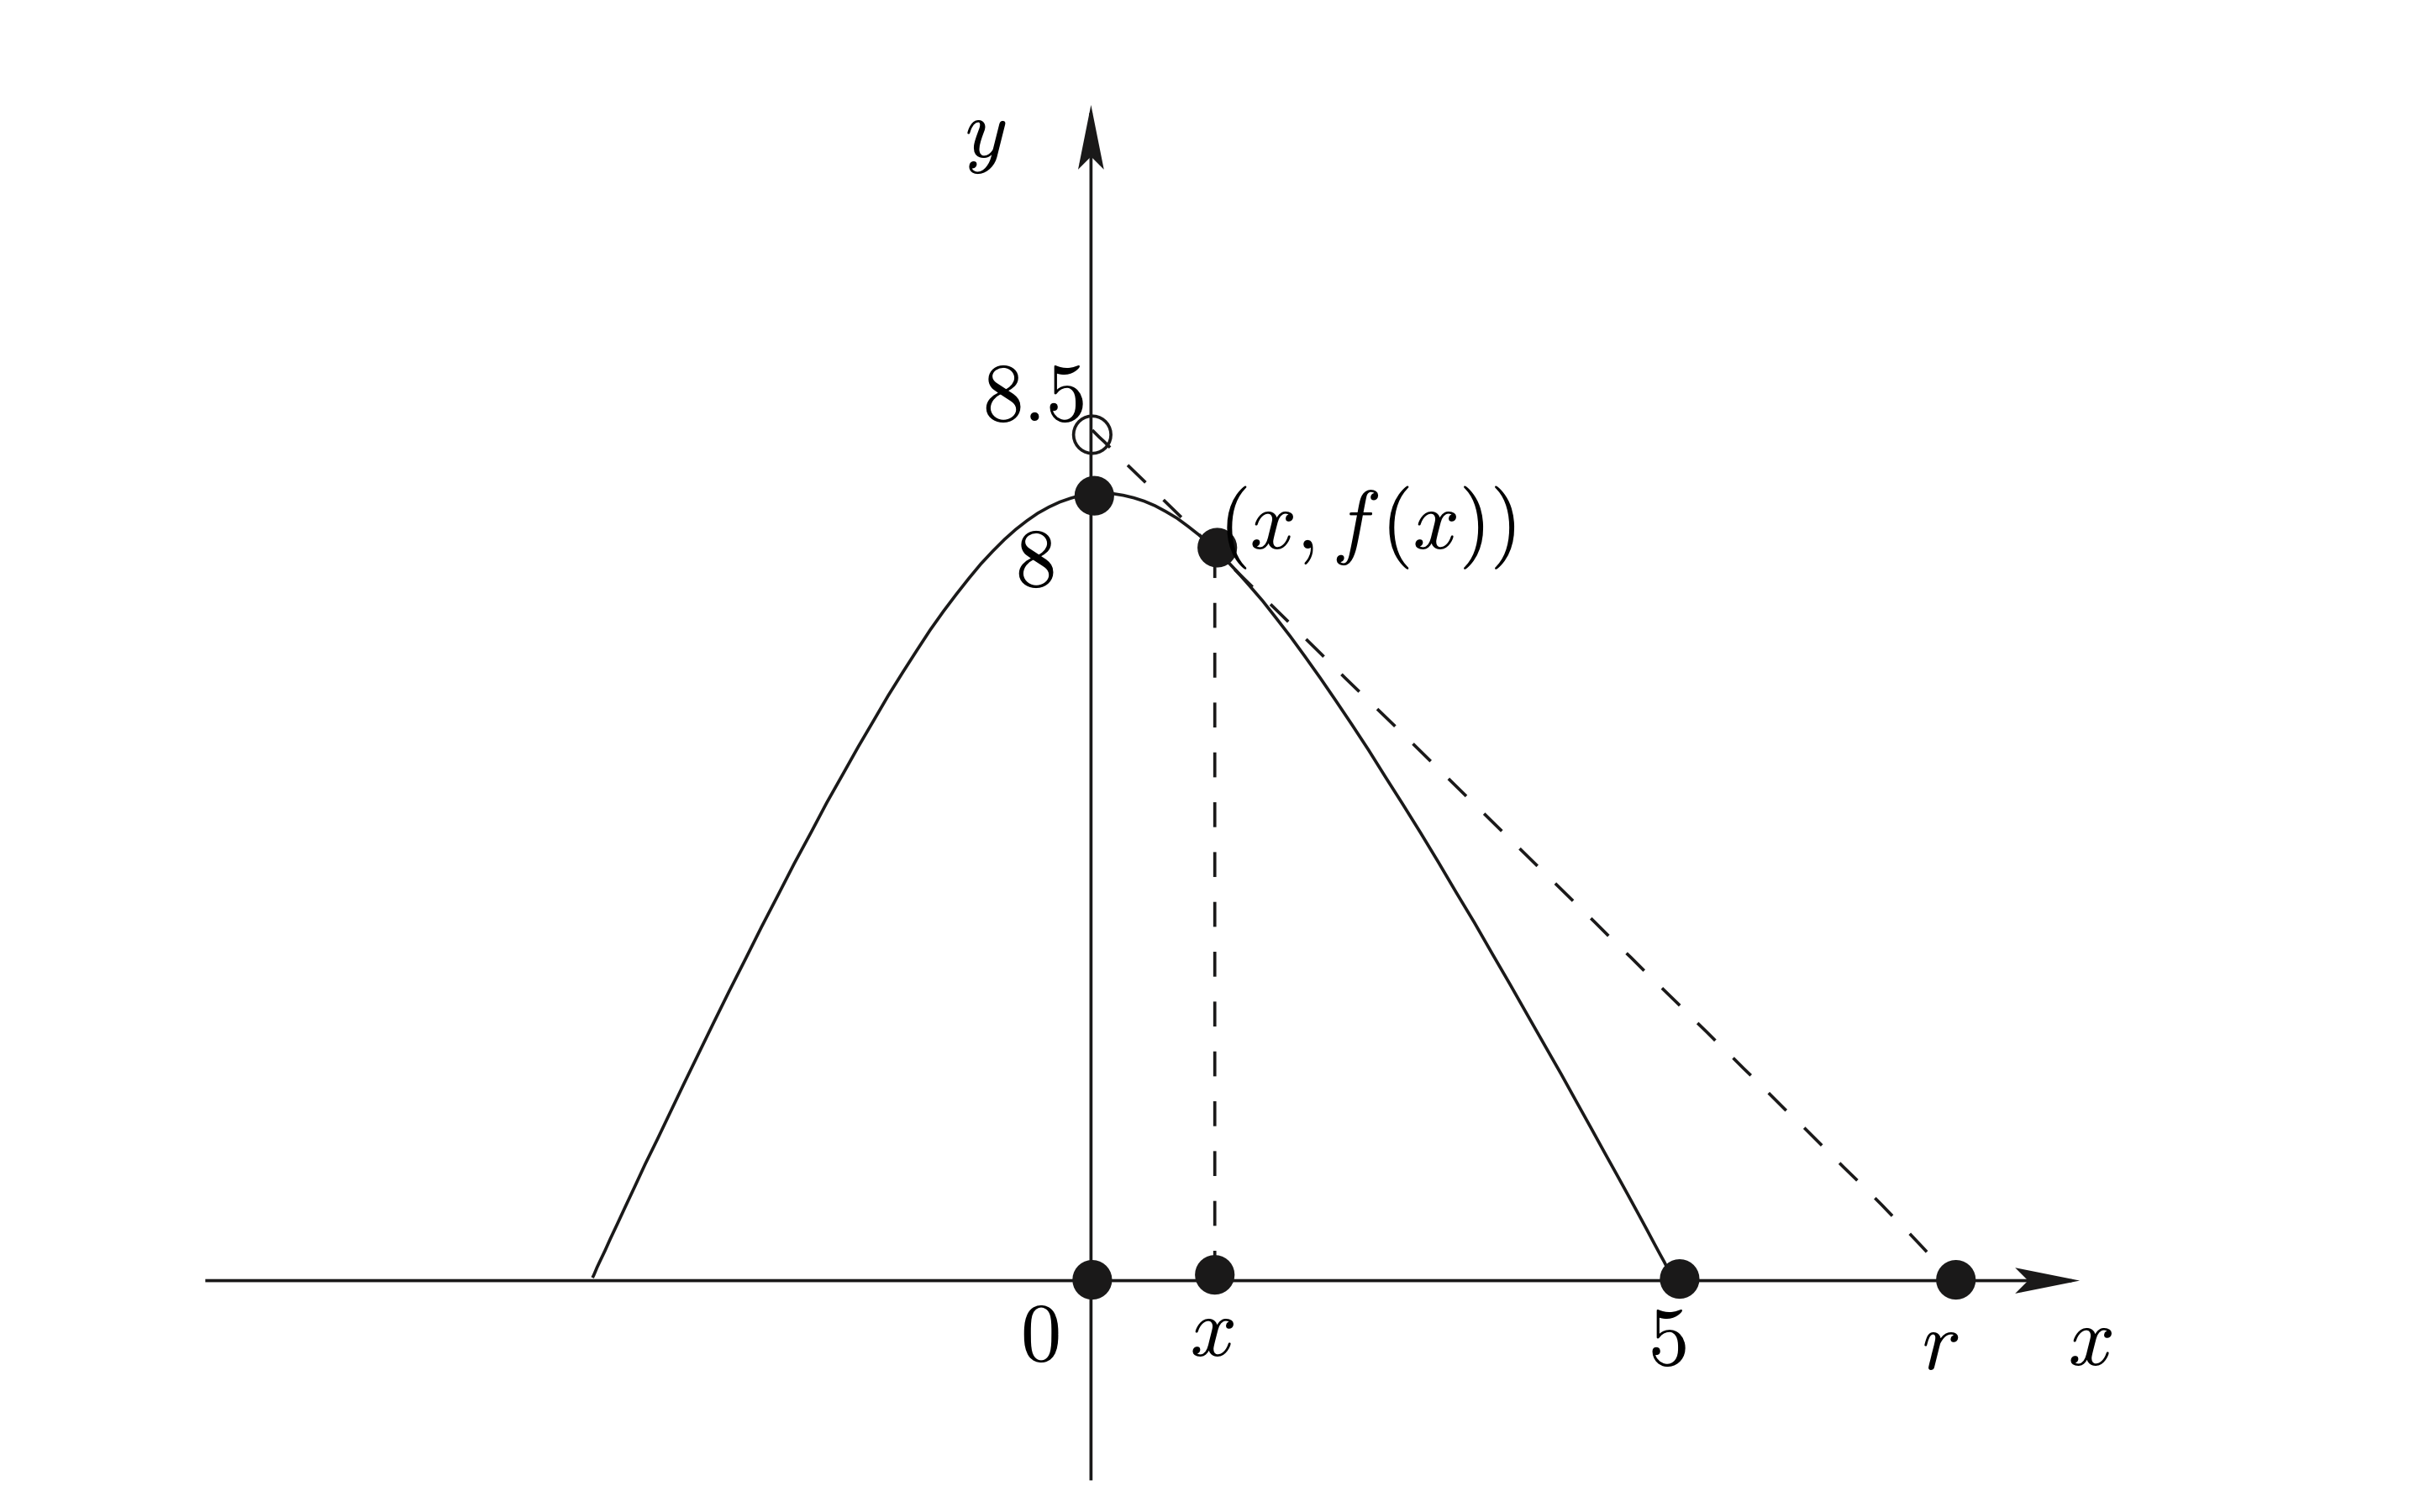
\includegraphics[width=0.5\linewidth]{images/fig-derivative-3} 

}

\caption{รูปภาพสำหรับตัวอย่างข้างต้น}\label{fig:fig-derivative-3}
\end{figure}

\subsection{อนุพันธ์ในเชิงอัตราเร็ว (Derivatives as Speeds)}\label{uxe2duxe19uxe1euxe19uxe18uxe43uxe19uxe40uxe0auxe07uxe2duxe15uxe23uxe32uxe40uxe23uxe27-derivatives-as-speeds}

ถ้าพิจารณาการเคลื่อนที่ของวัตถุ โดยให้ \(f(t)\) เป็นระยะทางที่วัตถุเคลื่อนที่ได้ ณ เวลา \(t\)
เราจะได้ว่า \(f'(t)\) ก็คืออัตราเร็ว ณ เวลา \(t\) ซึ่งเรียกว่า อัตราเร็วชั่วขณะ
(instantaneous speed) ในขณะที่ปริมาณ \(\displaystyle \frac{f(s)-f(t)}{s-t}\)
เรียกว่า อัตราเร็วเฉลี่ยของวัตถุ ในช่วงเวลา ตั้งแต่ \(s\) ถึง \(t\)

\begin{example}

วัตถุเคลื่อนที่เป็นเวลานาน 1 นาที ตามสมการ \(s=0.5t+0.1t^2\) เมื่อ \(t\) คือเวลาเป็นวินาที
และ \(s\) คือระยะทางที่เคลื่อนที่ได้เป็นเมตร จงหา

\begin{enumerate}
\def\labelenumi{(\arabic{enumi})}
\item
  อัตราเร็วเฉลี่ยของวัตถุในช่วง 10 วินาทีแรก และในช่วง 10 วินาทีถัดไป
\item
  อัตราเร็วของวัตถุ ณ วินาทีที่ 10 และ ณ วินาทีที่ 20
\end{enumerate}

\end{example}

\textbf{วิธีทำ}\\
(1) อัตราเร็วเฉลี่ยของวัตถุในช่วง 10 วินาทีแรก เท่ากับ\\
\(\displaystyle\frac{s(10)-s(0)}{10-0}
       =\frac{(0.5\times10+0.1\times10^2)-(0.5\times0+0.1\times0^2)}{10-0}=1.5\)
เมตรต่อวินาที\\
อัตราเร็วเฉลี่ยของวัตถุในช่วง 10 วินาทีถัดไป เท่ากับ\\
\(\displaystyle\frac{s(20)-s(10)}{20-10}
       =\frac{(0.5\times20+0.1\times20^2)-(0.5\times10+0.1\times10^2)}{20-10}=3.5\)
เมตรต่อวินาที\\
(2) เนื่องจาก
\(\displaystyle\frac{d}{dt}\left(0.5t+0.1t^2\right)=0.5+0.2t\)\\
ดังนั้น อัตราเร็วของวัตถุ ณ วินาทีที่ 10 เท่ากับ\\
\(\displaystyle\left.\frac{ds}{dt}\right|_{t=10}
       =\left.\frac{d}{dt}\left(0.5t+0.1t^2\right)\right|_{t=10}=0.5+0.2\times10=2.5\)
เมตรต่อวินาที\\
และ อัตราเร็วของวัตถุ ณ วินาทีที่ 20 เท่ากับ\\
\(\displaystyle\left.\frac{ds}{dt}\right|_{t=20}
       =\left.\frac{d}{dt}\left(0.5t+0.1t^2\right)\right|_{t=20}=0.5+0.2\times20=4.5\)
เมตรต่อวินาที

\subsection{อนุพันธ์ในเชิงอัตราการเปลี่ยนแปลง (Derivatives as Rates of Change)}\label{uxe2duxe19uxe1euxe19uxe18uxe43uxe19uxe40uxe0auxe07uxe2duxe15uxe23uxe32uxe01uxe32uxe23uxe40uxe1buxe25uxe22uxe19uxe41uxe1buxe25uxe07-derivatives-as-rates-of-change}

เราจะเห็นได้ชัดจากนิยามของอนุพันธ์ว่า ในกรณีของฟังก์ชันทั่วๆ ไป อนุพันธ์ของฟังก์ชัน
ก็คืออัตราการเปลี่ยนแปลงของค่าฟังก์ชัน เทียบกับตัวแปรต้นของมันนั่นเอง

\begin{example}
เมื่อใช้เครื่องสูบลม สูบลมเข้าไปในลูกโป่ง เราอาจประมาณได้ว่า ณ ขณะเวลาใดๆ
ลูกโป่งมีรูปร่างเป็นรูปทรงกลม จงหาอัตราการเพิ่มขึ้นของปริมาตรของลูกโป่ง
ต่อหนึ่งหน่วยรัศมีที่เพิ่มขึ้นของลูกโป่ง ขณะที่ลูกโป่งมีรัศมี 10 เซนติเมตร
\end{example}

\textbf{วิธีทำ} ให้ \(r\) เป็นรัศมีของลูกโป่ง และ \(V\) เป็นปริมาตรของลูกโป่ง
จากข้อสมมุติว่าลูกโป่งเป็นทรงกลม จะได้ว่า \(V=4\pi r^3/3\) ดังนั้น
อัตราการเปลี่ยนแปลงของปริมาตรของลูกโป่งเทียบกับรัศมีเท่ากับ
\(\displaystyle\frac{dV}{dr}=12\pi r^2/3=4\pi r^2\) ลูกบาศก์หน่วยต่อหน่วย นั่นคือ
ขณะที่ลูกโป่งมีรัศมี 10 เซนติเมตร มันจะมีปริมาตรเพิ่มขึ้นในอัตรา
\(4\times\pi\times10^2\approx1256\) ลูกบาศก์เซนติเมตรต่อเซนติเมตร หรือประมาณ
\(1.256\) ลิตรต่อรัศมีที่เพิ่มขึ้น 1 เซนติเมตร

\subsection{แบบฝึกหัด (Exercises)}\label{uxe41uxe1auxe1auxe1duxe01uxe2buxe14-exercises}

\begin{enumerate}
\def\labelenumi{\arabic{enumi}.}
\item
  จงหาอนุพันธ์ต่อไปนี้ ถ้าอนุพันธ์ดังกล่าวหาค่าได้ ในกรณีที่หาค่าไม่ได้ ให้ระบุว่าหาค่าไม่ได้

  \begin{enumerate}
  \def\labelenumii{\arabic{enumii}.}
  \item
    \(\displaystyle f'(x)\) เมื่อ \(f(x)=g(x)h(x)k(x)\)
  \item
    \(\displaystyle f^{(n)}(0)\) เมื่อ
    \(\displaystyle f(x)=\sum_{i=1}^k x^i\) โดยที่ \(k\) และ \(n\)
    เป็นจำนวนนับ
  \item
    \(\displaystyle\frac{d}{dt}\frac1{1-t}\) และ
    \(\displaystyle\frac{d^2}{dt^2}\frac1{1-t}\)
  \item
    \(\displaystyle\frac{d}{dt}\frac{f(t)}t\) เมื่อ \(f\) เป็นฟังก์ชันซึ่ง
    \(\displaystyle\frac{d}{dt}f(t)=\frac{f(t)}t\) สำหรับทุกๆ \(t\neq0\)
  \item
    \(f'(-1)\), \(f'(-\frac23)\), \(f'(0)\), \(f'(1)\) เมื่อ
    \(f(x)=x\sqrt{1+x}\)
  \item
    \(\displaystyle\left.\frac d{dx}\,\frac x{\sqrt{1+x}-\sqrt{1-x}}\right|_{x=0}\)
  \item
    \(\displaystyle\frac {dy}{dx}\;\),
    \(\displaystyle\left.\frac {dy}{dx}\,\right|_{x=0}\),
    \(\displaystyle\left.\frac {dy}{dx}\,\right|_{x=0.25}\),
    \(\displaystyle\left.\frac {dy}{dx}\,\right|_{x=1}\) เมื่อ
    \(\displaystyle y=\frac{1-\sqrt x}{\sqrt{1-x}}\)
  \item
    \(\displaystyle\frac d{dx}\,\left(x^2\sqrt{1+x}\right)\)
  \item
    \(\displaystyle\frac {d^2y}{dx^2}\) เมื่อ \(y=(1+x^2)\sqrt{1-2x}\) (
    หาอนุพันธ์ของ \(\sqrt{1-2x}\) และ \(1/\sqrt{1-2x}\) ก่อน)
  \item
    \(\displaystyle\frac {d^{10}y}{dx^{10}}\) เมื่อ
    \(y=\left(x^5-x^4-x^3-x^2-x-1\right)\left(x^5+2x^4+2x^3+2x^2+2x+2\right)\)
  \end{enumerate}
\item
  จงตอบคำถามต่อไปนี้

  \begin{enumerate}
  \def\labelenumii{\arabic{enumii}.}
  \item
    จงหาความชันของกราฟของสมการ \(y=x^3-3x\) ณ ตำแหน่งซึ่ง \(x=2\)
  \item
    จงหาจุดบนกราฟ \(y=x^3-3x\) ซึ่งมีเส้นสัมผัสกราฟที่ขนานกับเส้นสัมผัส ณ จุดซึ่ง
    \(x=a\) เมื่อ \(a\) เป็นจำนวนจริงใดๆ
  \item
    จงหาจุดบนกราฟ \(y=x^3-3x\) ซึ่งมีเส้นสัมผัสกราฟที่ตั้งฉากกับเส้นสัมผัส ณ จุดซึ่ง
    \(x=a\) เมื่อ \(a\) เป็นจำนวนจริงใดๆ
  \end{enumerate}
\end{enumerate}

\section{กฎลูกโซ่ (The Chain Rule)}\label{uxe01uxe0euxe25uxe01uxe42uxe0b-the-chain-rule}

การทราบข้อมูลของ derivative ของฟังก์ชัน \(f\) และฟังก์ชัน \(g\) ทำให้เราสามารถหา
derivative ของผลบวก \(f+g\) ผลคูณ \(fg\) และผลหาร \(f/g\) ของฟังก์ชัน ทั้งสองได้
ข้อมูลนี้ยังใช้หา derivative ของฟังก์ชันประกอบ \(f\circ g\) ภายใต้เงื่อนไขที่เหมาะสมได้
เราเรียกวิธีการหา derivative ของฟังก์ชัน ประกอบว่า chain rule โดยมีแนวคิดสำคัญคือ
การสร้างตัวแปรใหม่ขึ้นมาช่วย ในการคำนวณ ดังรายละเอียดในทฤษฏีบทต่อไปนี้

\begin{theorem}
ถ้าฟังก์ชัน \(g\) หา derivative ได้ที่จุด \(x\) และฟังก์ชัน \(f\) หา derivative ได้ที่จุด
\(g(x)\) แล้ว ฟังก์ชันประกอบ \(f \circ g\) หา derivative ได้ที่จุด \(x\) ยิ่งกว่านั้น ถ้า
\[y = f(g(x)) \quad \text{และ} \quad u = g(x)\] แล้ว \(y=f(u)\) และ
\[\label{E:chain1}
\boxed{
    \frac{dy}{dx} = \frac{dy}{du} \cdot \frac{du}{dx}
}\]
\end{theorem}

ตัวอย่างต่อไปนี้แสดงให้เห็นถึงการใช้ chain rule หา derivative ของฟังก์ชัน

\begin{example}
พิจารณาฟังก์ชัน \(y = \frac{1}{x^2+1}\) กำหนดให้ \(u = x^2+1\) จงหา
\(\frac{dy}{dx}\)
\end{example}

\textbf{วิธีทำ} ในที่นี้ \(y = \frac{1}{u}\) เราใช้ chain rule ได้ว่า
\begin{equation}   \begin{aligned}
    \frac{dy}{dx}
    &= \frac{dy}{du} \cdot \frac{du}{dx} \\
    &= \frac{d}{du}\left[\frac{1}{u}\right] \cdot \frac{d}{dx}[x^2+1] \\
    &= \left(-\frac{1}{u^2}\right) \cdot (2x) \\
    &= -\frac{1}{(x^2+1)^2} \cdot (2x) \\
    &= -\frac{2x}{(x^2+1)^2}
  \end{aligned} \end{equation} นั่นคือ
\(\displaystyle \frac{dy}{dx} = -\frac{2x}{(x^2+1)^2}\)

\begin{example}
กำหนดให้ \(y = u^{100}\) และ \(u = x^3 + x^2 + x + 1\) จงหา \(\frac{dy}{dx}\)
\end{example}

\textbf{วิธีทำ} ใช้ chain rule ได้ว่า \begin{equation}   \begin{aligned}
    \frac{dy}{dx}
    &= \frac{dy}{du} \cdot \frac{du}{dx} \\
    &= \frac{d}{du}[u^{100}] \cdot \frac{d}{dx}[x^3+x^2+x+1] \\
    &= (100u^{99}) \cdot (3x^2+2x+1) \\
    &= 100(x^3+x^2+x+1)^{99}(3x^2+2x+1)
  \end{aligned} \end{equation} นั่นคือ
\(\displaystyle \frac{dy}{dx} = 100(x^3+x^2+x+1)^{99}(3x^2+2x+1)\)

\textbf{ข้อสังเกต} สูตรของกฎลูกโซ่สามารถเขียนได้ในอีกรูป ซึ่งสะดวกในการนำไปใช้ สังเกตว่า
\(y = f(u)\) ดังนั้น
\[\frac{dy}{dx} = \frac{d}{dx}[f(u)] \quad \text{และ} \quad
    \frac{dy}{du} = f'(u)\] สูตรของ chain rule จึงเขียนได้ว่า
\[\label{E:chain2}
\boxed{
    \frac{d}{dx}[f(u)] = f'(u)\frac{du}{dx}
}\] ซึ่งเขียนได้อีกรูปคือ \[\frac{d}{dx} f(g(x)) = f'(g(x))\cdot g'(x)\]

\begin{example}
จงหา derivative ของฟังก์ชัน \(y = \sqrt{\frac{1}{2}x^2+x+1}\)
\end{example}

\textbf{วิธีทำ} เราแนะนำตัวแปร \(u = \frac{1}{2}x^2+x+1\) และใช้สูตร chain rule ได้ว่า \begin{equation}   \begin{aligned}
    \frac{d}{dx} \left[\sqrt{\frac{1}{2}x^2+x+1} \right]
    &= \frac{d}{dx}[\sqrt{u}] \\
    &= \frac{d}{du}\sqrt{u} \cdot \frac{du}{dx} \\
    &= \frac{1}{2\sqrt{u}} \frac{du}{dx} \\
    &= \frac{1}{2\sqrt{\frac{1}{2}x^2+x+1}} \frac{d}{dx}
\left[\frac{1}{2}x^2+x+1\right] \\
    &= \frac{1}{2\sqrt{\frac{1}{2}x^2+x+1}} \cdot (x+1) \\
    &= \frac{x+1}{2\sqrt{\frac{1}{2}x^2+x+1}}
  \end{aligned} \end{equation} นั่นคือ
\(\displaystyle \frac{dy}{dx} = \frac{x+1}{2\sqrt{\frac{1}{2}x^2+x+1}}\)

\begin{example}
จงหาค่าของ \(f'(x^3+x)\) เมื่อกำหนดให้ \[\frac{d}{dx}[f(x^3+x)] = (3x^2+1)^2\]
\end{example}

\textbf{วิธีทำ} เราใช้ chain rule ได้ว่า \begin{equation}   \begin{aligned}
    \frac{d}{dx}[f(x^3+x)]
    &= f'(x^3+x) \frac{d}{dx} [x^3+x] \\
    &= f'(x^3+x) \cdot (3x^2+1)
  \end{aligned} \end{equation} ดังนั้น
\[(3x^2+1)^2 = f'(x^3+x)\cdot(3x^2+1)\] หรือ \[f'(x^3+x) = 3x^2+1\]
สังเกตความแตกต่างระหว่าง \(\displaystyle \frac{d}{dx} f(x^3+x)\) และ
\(f'(x^3+x)\)

\begin{example}
กำหนดให้ \(f(x) = |x|\) จงหา derivative ของฟังก์ชัน \(f\) ที่ \(x \ne 0\)
\end{example}

\textbf{วิธีทำ} ฟังก์ชัน \(f\) เขียนได้ว่า \[f(x) = |x| = \sqrt{x^2}\] ถ้า \(x\ne 0\) แล้ว
\begin{equation}   \begin{aligned}
    f'(x) &= \frac{d}{dx} \sqrt{x^2} \\
          &= \frac{d}{du} [\sqrt{u}] \cdot \frac{d}{dx} [x^2] \\
          &= \frac{1}{2\sqrt{u}} \cdot (2x) \\
          &= \frac{1}{\sqrt{x^2}} \cdot x \\
          &= \frac{x}{|x|}
  \end{aligned} \end{equation} นั่นคือ เมื่อ \(x\ne 0\) แล้ว
\(\displaystyle f'(x) = \frac{x}{|x|}\)

\subsection{แบบฝึกหัด}\label{uxe41uxe1auxe1auxe1duxe01uxe2buxe14}

\begin{enumerate}
\def\labelenumi{\arabic{enumi}.}
\item
  จงหา derivative ของฟังก์ชันต่อไปนี้

  \begin{enumerate}
  \def\labelenumii{\arabic{enumii}.}
  \item
    \(\displaystyle f(x) = \sqrt{1-x+x^2}\)
  \item
    \(\displaystyle f(x) = \frac{1}{1+x+x^2}\)
  \item
    \(\displaystyle f(x) = (2x+5)^3(3x-7)^5\)
  \item
    \(\displaystyle f(x) = \frac{x^2+1}{x^3+x^2+1}\)
  \end{enumerate}
\item
  จงหา derivative ของฟังก์ชัน
  \[y = \sqrt{x + \sqrt[3]{3x + \sqrt[4]{4x}}}\]
\item
  กำหนดให้ \(f\) เป็นฟังก์ชันหา derivative ได้ และ \(g = f \circ f\) ถ้า
  \(f(1) = 1\), \(f(2) = 4\) และ \(f'(4) = 8\) จงหาค่าของ \(g'(1)\)
\item
  พิจารณาตารางค่าของฟังก์ชัน \(f, f'\), \(g, g'\) และ \(h, h'\) โดยที่ \(h=f\circ g\)

  \begin{longtable}[]{@{}ccccccc@{}}
  \toprule\noalign{}
  \(x\) & \(f(x)\) & \(g(x)\) & \(h(x)\) & \(f'(x)\) & \(g'(x)\) & \(h'(x)\) \\
  \midrule\noalign{}
  \endhead
  \bottomrule\noalign{}
  \endlastfoot
  -1 & 0 & 1 & 2 & 2 & 0 & 2 \\
  0 & 3 & -1 & ? & 1 & 1 & ? \\
  1 & ? & 0 & 0 & ? & ? & 3 \\
  \end{longtable}

  จงหาค่าของ \(h(0)\), \(f(1)\), \(h'(0)\), \(f'(1)\) และ \(g'(1)\)
\item
  จาก chain rule~\hyperref[E:chain1]{\[E:chain1\]},
  \(\frac{dy}{dx} = \frac{dy}{du} \cdot \frac{du}{dx}\), จงหาสูตร ของ
  \(\displaystyle \frac{d^2y}{dx^2}\)
\end{enumerate}

\section{อนุพันธ์ของฟังก์ชันอินเวอร์ส (Derivatives of Inverse Functions)}\label{uxe2duxe19uxe1euxe19uxe18uxe02uxe2duxe07uxe1fuxe07uxe01uxe0auxe19uxe2duxe19uxe40uxe27uxe2duxe23uxe2a-derivatives-of-inverse-functions}

\begin{definition}
ถ้าฟังก์ชัน \(f\) และ \(g\) สอดคล้องสมบัติ

\begin{enumerate}
\def\labelenumi{\arabic{enumi}.}
\item
  \(g(f(x)) = x\) สำหรับ \(x\) ที่เป็นสมาชิกของโดเมนของ \(f\)
\item
  \(f(g(y)) = y\) สำหรับ \(y\) ที่เป็นสมาชิกของโดเมนของ \(g\)
\end{enumerate}

เรากล่าวว่า \(f\) และ \(g\) เป็นฟังก์ชันอินเวอร์ส โดยที่ \(f\) เป็น ฟังก์ชันอินเวอร์สของ \(g\)
และ \(g\) เป็นฟังก์ชันอินเวอร์ส ของ \(f\)
\end{definition}

ถ้าเขียน \(f^{-1}\) แทน \(g\) และใช้สัญกรณ์ \(x\) แทนสมาชิกทั้งในโดเมนของ \(f\) และ
\(f^{-1}\) สมมติว่าทั้งสองฟังก์ชันหา derivative ได้ ให้ \[y = f^{-1}(x)\]
เราสามารถเขียนใหม่ได้ว่า \[x = f(y)\] หา derivative เทียบกับ \(x\)
\begin{equation}   \begin{aligned}
    \frac{d}{dx}[x]
    &= \frac{d}{dx}[f(y)] \\
    &= f'(y) \cdot \frac{dy}{dx}
  \end{aligned} \end{equation} นั่นคือ \[1 = f'(y) \cdot \frac{dy}{dx}\]
หรือ \[\frac{dy}{dx} = \frac{1}{f'(y)}\] เขียนใหม่ได้ว่า \[\label{E:inverse}
\boxed{
    \frac{d}{dx}[f^{-1}(x)] = \frac{1}{f'(f^{-1}(x))}
}\]

\begin{example}
กำหนดให้ \(f(x) = x^3\) มี \(f^{-1}(x) = x^{1/3}\) จงหา
\(\frac{d}{dx} [f^{-1}(x)]\)
\end{example}

\textbf{วิธีทำ} คำนวณหา derivative ได้ว่า \(f'(x) = 3x^2\) และ
\begin{equation}   \begin{aligned}
    \frac{d}{dx} [x^{1/3}]  = \frac{d}{dx} [f^{-1}(x)]
    &= \frac{1}{3[f^{-1}(x)]^2} \\
    &= \frac{1}{3[x^{1/3}]^2} \\
    &= \frac{1}{3x^{2/3}}
  \end{aligned} \end{equation}

ในการหา derivative ของฟังก์ชันอินเวอร์ส เราอาจจะไม่ใช้สูตรโดยตรง แต่ จะคำนวณหา
derivative ตามขั้นตอนที่ได้แสดงข้างต้น ดังตัวอย่าง

\begin{example}
พิจารณาฟังก์ชัน \(f(x) = x^3+x+2\) จงหา derivative ของ \(f^{-1}(x)\)
\end{example}

\textbf{วิธีทำ} เราเขียน \(x = f(y) = y^3+y+2\) แล้วหา derivative เทียบกับ \(x\)
\begin{equation}   \begin{aligned}
    \frac{d}{dx}[x]  &= \frac{d}{dx}[y^3+y+2] \\
    1 &= (3y^2+1)\frac{dy}{dx}
  \end{aligned} \end{equation} ดังนั้น
\(\displaystyle \frac{dy}{dx} = \frac{1}{3y^2+1}\)

\begin{example}
กำหนดให้ \(f\) เป็นฟังก์ชันซึ่งมีอิสเวอร์ส ถ้า \(f(1) = 2\) และ \(f'(1) = 3\) แล้ว
จงหาค่าของ \((f^{-1})'(2)\)
\end{example}

\textbf{วิธีทำ} เนื่องจาก \(f(1) = 2\) แล้ว \(f^{-1}(2) = 1\) และจากสูตร
~\hyperref[E:inverse]{\[E:inverse\]} \begin{equation}   \begin{aligned}
    (f^{-1})'(2)
    &= \frac{1}{f'(f^{-1}(2))} \\
    &= \frac{1}{f'(1)} \\
    &= \frac{1}{3}
  \end{aligned} \end{equation} นั่นคือ \(\displaystyle (f^{-1})'(2) = 1/3\)

\subsection{แบบฝึกหัด}\label{uxe41uxe1auxe1auxe1duxe01uxe2buxe14-1}

\begin{enumerate}
\def\labelenumi{\arabic{enumi}.}
\item
  จงหา \((f^{-1})'(x)\) เมื่อกำหนด

  \begin{enumerate}
  \def\labelenumii{\arabic{enumii}.}
  \item
    \(\displaystyle f(x) =  2x^3-1\)
  \item
    \(\displaystyle f(x) = \frac{x+1}{x-1}\)
  \item
    \(\displaystyle f(x) = \frac{x^3+1}{x^2+1}\)
  \item
    \(\displaystyle f(x) = \sqrt{x^3+x^2+x+1}\)
  \end{enumerate}
\end{enumerate}

\section{Differentials, Implicit Differentiation and Related Rates}\label{differentials-implicit-differentiation-and-related-rates}

\subsection{Differentials}\label{differentials}

ที่ผ่านมา เราให้ความหมายของ \(dy/dx\) ว่าเป็น derivative ของ \(y\) เทียบกับ \(x\)
ในความหมายของตัวดำเนินการ \(\frac{d}{dx}\) ที่กระทำ กับฟังก์ชัน \(y\) หัวข้อนี้เราจะนิยาม
\(dy\) และ \(dx\) แยกจากกัน และให้ความหมาย \(dy/dx\) ว่าเป็นเศษส่วน\\
\strut \\
ผลต่างระหว่างค่าสองค่าของตัวแปร เราเรียกว่า increment เช่นในตัวแปร \(x\)
ผลต่างระหว่างค่า \(x=x_0\) และ \(x=x_1\) เราเขียน increment ใน \(x\) นี้ ว่า
\(\Delta x = x_1-x_0\)\\
\strut \\
ให้ \(y=f(x)\) และให้ \(x\) มีการเปลี่ยนค่าจาก \(x=x_0\) ไปยัง \(x=x_1\) ก็จะมี
การเปลี่ยนค่าใน \(y\) จาก \(y_0 = f(x_0)\) ไปยัง \(y_1= f(x_1)\) นั่นหมายความ ว่า
increment \(\Delta x\) ทำให้เกิด increment \(\Delta y = y_1-y_0\) โดยที่
\[\Delta y = y_1-y_0 = f(x_1) - f(x_0)\] หรือ
\[\Delta y = f(x_0+\Delta x) - f(x_0)\] ดังนั้น สำหรับค่า \(x\) ทั่วไปแล้ว
เราอาจเขียน \[\Delta y = f(x+ \Delta x) - f(x)\] และนิยามของ derivative
ก็เขียนได้อีกรูปว่า
\[\frac{dy}{dx} = \lim_{\Delta x \to 0} \frac{\Delta y}{\Delta x} \\
    = \lim_{\Delta x \to 0} \frac{f(x+\Delta x) - f(x)}{\Delta x}\]

เมื่อเราเห็นการเขียนสัญกรณ์ \(\displaystyle \frac{dy}{dx}\) มีแนวโน้มที่จะ
ทำให้เราคิดถึงผลหารของ \(dy\) ด้วย \(dx\) ซึ่งในขณะนี้ ทั้งสองปริมาณยังไม่มี ความหมายใด ๆ
สังเกตว่าในสูตรของ chain rule ที่ว่า
\(\displaystyle \frac{dy}{dx} = \frac{dy}{du} \cdot \frac{du}{dx}\) ก็ให้
ความรู้สึกแรกว่าน่าจะเป็นผลหารเช่นกัน ดังนั้นลำดับถัดไปเราจะให้ความหมายของ พจน์ \(dx\),
\(dy\) และการตีความหมายในรูปเศษส่วน\\
\strut \\
เริ่มด้วยการตรึงค่า \(x\) และนิยาม \(dx\) ว่าเป็นตัวแปรต้น กำหนดให้ \(y = f(x)\) และ \(f\)
เป็นฟังก์ชัน หา derivative ได้ เรานิยาม \(dy\) ว่าเป็นตัวแปรตามดังนี้ \[\boxed{
    dy = f'(x)\,dx
}\] ถ้า \(dx \ne 0\) เราเขียนใหม่ได้ว่า \[\frac{dy}{dx} = f'(x)\] เราเรียก \(dy\)
ว่า differential ของ \(y\) และ \(dx\) ว่า differential ของ \(x\)\\
\strut \\
มีความแตกต่างระหว่าง ความหมายของ differential \(dy\) และ increment
\(\Delta y = y_1-y_0\) ถ้าเรากำหนดให้ differential \(dx\) และ increment
\(\Delta x\) มีค่า เดียวกัน นั่นคือ \(dx = \Delta x\) จะเห็นว่า \(\Delta y\) แทนถึง
ค่าผลต่างใน \(y\) ของจุดเริ่มต้น \(x\) และจุดปลาย \(x+\Delta x\) ตามเส้นโค้ง \(y = f(x)\)
นั่นคือ \(\Delta y = f(x+\Delta x) - f(x)\) ในขณะที่ \(dy\) แทนถึงค่าผลต่างใน \(y\)
ของจุดเริ่มต้น \(x\) และจุดปลาย \(x+\Delta
x\) ตามเส้นสัมผัสของเส้นโค้ง \(y=f(x)\) ที่ผ่านจุด \((x,f(x))\) และ มีความชันเท่ากับ
\(f'(x)\)

\begin{example}
ถ้า \(y = f(x) = x^2+1\) แล้ว \(f'(x) = 2x\) กำหนดให้ \(x=3\) จงหาค่าของ \(dy\) และ
\(\Delta y\) เมื่อ \(dx = \Delta x = 0.1\)
\end{example}

\textbf{วิธีทำ} ค่าของ \(dy\) คือ \[dy = f'(x) \,dx = 2x\,dx\] กรณีตรึง \(x=3\) ได้ว่า
\[dy = 6\,dx\] ถ้าให้ \(dx=0.1\) ค่าของ \(dy = 0.6\) ถ้าเราพิจารณาค่า
\(dx = \Delta x= 0.1\) เราก็จะได้
\[\Delta y = f(3+\Delta x) - f(3) = (3.1)^2+1 - 3^2-1 = 0.61\] สังเกตว่า
\(dy = 0.6\) ในขณะที่ \(\Delta y = 0.61\)

มีข้อสังเกตว่า ถ้า \(f\) เป็นฟังก์ชันหา derivative ได้ที่ค่า \(x_0\) แล้วเส้นสัมผัส กับเส้นโค้ง
\(y= f(x)\) ที่จุด \((x_0,f(x_0))\) จะใกล้เคียงกับกราฟของ \(f\) สำหรับค่า \(x\) ใกล้ ๆ
กับค่า \(x_0\) สมการเส้นสัมผัสกับเส้นโค้งนี้ที่ผ่านจุด \((x_0,f(x_0))\) มี ความชัน \(f'(x_0)\)
คือ \[y = f(x_0) + f'(x_0)(x-x_0)\] เมื่อเรากล่าวว่า เส้นโค้ง \(y=f(x)\)
และเส้นสัมผัสกับเส้นใกล้เคียงกันหมายถึงถ้าเรา ให้ \(x\) เข้าใกล้ \(x_0\) ค่าของ
\(f(x_0)+f'(x_0)(x-x_0)\) ก็จะใกล้เคียงค่า \(f(x)\) \[\label{E:approx}
    f(x) \approx  f(x_0) + f'(x_0)(x-x_0)\]
เราเรียกสมการ~\hyperref[E:approx]{\[E:approx\]} ว่า local linear approximation ของ \(f\) ที่ \(x_0\) เรา
อาจเขียนในอีกรูปว่า \[f(x_0 + \Delta x) \approx f(x_0) + f'(x_0)\Delta x\]

\begin{example}
จงหา local linear approximation ของฟังก์ชัน \(f(x) = x^{1/3}\) ที่ \(x_0 = 1\)
\end{example}

\textbf{วิธีทำ} เรามี \(f(x) = x^{1/3}\) และคำนวณหา derivative
\[f'(x) = \frac{1}{3}x^{-2/3}\] local linear approximation ของ \(f\) ที่
\(x_0 = 1\) จึงเป็น
\[x^{1/3} \approx 1 + \frac{1}{3}(x-1) = \frac{1}{3}x+\frac{2}{3}\]
ถ้าเราต้องการประมาณค่าของ \((1.1)^{1/3}\) เราใช้ local linear approximation
ของ \(f\) ในการประมาณ โดยได้ค่าประมาณคือ \(1+\frac{1}{3}(1.1-1) = 1.03\)

\subsection{Implicit Differentiation}\label{implicit-differentiation}

บางครั้งเราต้องการหา derivative ของฟังก์ชัน ซึ่งไม่สามารถเขียนได้ ในรูปฟอร์ม
\(y = f(x)\) เช่นในความสัมพันธ์ \[x^2+y^3 - xy = 0\] การหา derivative ของ \(y\)
เทียบกับ \(x\) เราไม่จำเป็นต้องเขียนความสัมพันธ์ ให้อยู่ในรูป \(y = f(x)\) ก่อน
หลักการสำคัญก็คือ เราคิดให้ \(y\) เป็น ฟังก์ชันของ \(x\) เช่นในตัวอย่างที่ยกมา ถ้าเราหา
derivative ทั้งสองข้าง ของสมการเทียบกับ \(x\)
\begin{equation}   \begin{aligned}
    \frac{d}{dx}[x^2+y^3-xy] &= \frac{d}{dx}[0] \\
    \frac{d}{dx}[x^2] + \frac{d}{dx}[y^3] - \frac{d}{dx}[xy] &= 0 \\
    2x + 3y^2 \frac{dy}{dx} - x\frac{dy}{dx} -y &= 0
  \end{aligned} \end{equation} เขียนใหม่ได้ว่า
\[\frac{dy}{dx} = \frac{2x-y}{x-3y^2}\]

\begin{example}
กำหนดให้ \(y^2 = x^3(2-x)\) สังเกตว่า \((x,y) = (1,1)\) อยู่บน กราฟของความสัมพันธ์
จงหาว่าความชันของกราฟนี้ที่จุด \((1,1)\)
\end{example}

\textbf{วิธีทำ} หา derivative เทียบกับ \(x\) ทั้งสองข้าง ของสมการ
\begin{equation}   \begin{aligned}
    \frac{d}{dx}[y^2] &= \frac{d}{dx}[x^3(2-x)] \\
    \frac{d}{dy}[y^2] \cdot \frac{dy}{dx} &= x^3\frac{d}{dx}[2-x] + (2-x)\frac{d}{dx}[x^3] \\
    (2y) \cdot \frac{dy}{dx} &= -x^3 + (2-x)(3x^2) \\
    \frac{dy}{dx} &= \frac{(2-x)(3x^2)}{2y}
  \end{aligned} \end{equation} ดังนั้นที่จุด \((x,y) = (1,1)\) เราจะได้
derivative ของ \(y\) เทียบ กับ \(x\) เป็น
\(\displaystyle \frac{dy}{dx} = \frac{3}{2}\)

\begin{example}
จงหาสมการเส้นสัมผัสกับเส้นโค้งของสมการ \[xy^2 = 1\] ที่จุด \((1,-1)\)
\end{example}

\textbf{วิธีทำ} เริ่มด้วยการหาความชันของเส้นสัมผัสที่จุด \((1,-1)\) เราหา derivative
ของสมการเทียบกับ \(x\) ได้ว่า \begin{equation}   \begin{aligned}
    \frac{d}{dx}[xy^2] &= \frac{d}{dx}[1] \\
    x\frac{d}{dx}[y^2] + y^2\frac{d}{dx}[x] &= 0 \\
    x(2y)\frac{dy}{dx} + y^2 &= 0 \\
    \frac{dy}{dx} &= -\frac{y}{2x}
  \end{aligned} \end{equation} ดังนั้นความชันของเส้นสัมผัสที่จุด \((1,-1)\) มีค่าเท่ากับ
\(1/2\) สมการเส้น สัมผัสของเส้นโค้งที่จุด \((1,-1)\) จึงเป็น
\begin{equation}   \begin{aligned}
    \frac{y-(-1)}{x-1} &= \frac{1}{2} \\
    y+1 &= \frac{1}{2}x -\frac{1}{2}
  \end{aligned} \end{equation} นั่นคือ \(\displaystyle y=\frac{x-3}{2}\)

\begin{example}
พิจารณาสมการ \[\frac{1}{3}x^3+y^3-xy^2 = 5\]
จงหาว่าที่จุดใดบนเส้นโค้งที่เส้นสัมผัสขนานแกน \(x\)
\end{example}

\textbf{วิธีทำ} เราเริ่มด้วยการหา derivative ของสมการ
\begin{equation}   \begin{aligned}
    \frac{d}{dx} [\frac{1}{3}x^3 + y^3 -xy^2] &= \frac{d}{dx}[5] \\
    \frac{d}{dx}[\frac{1}{3}x^3] + \frac{d}{dx}[y^3] - \frac{d}{dx}[xy^2] &= 0 \\
    x^2 + 3y^2\frac{dy}{dx} - x\frac{d}{dx}[y^2] - y^2 &= 0 \\
    x^2 + 3y^2\frac{dy}{dx} - x(2y)\frac{dy}{dx} - y^2 &= 0 \\
    \frac{dy}{dx} &= \frac{y^2-x^2}{3y^2-2xy}
  \end{aligned} \end{equation} สังเกตว่าเส้นสัมผัสที่ขนานแกน \(x\) จะมีความชันเป็น 0
ดังนั้นที่จุดบน เส้นโค้งซึ่งมีเส้นสัมผัสขนานแกน \(x\) สอดคล้องกับสมการ
\begin{equation}   \begin{aligned}
    y^2-x^2 &= 0 \quad \text{และ}\\
    \frac{1}{3}x^3+y^3-xy^2 &= 5
  \end{aligned} \end{equation} เนื่องจาก \(y^2-x^2 = (y-x)(y+x) = 0\)

\begin{enumerate}
\def\labelenumi{\arabic{enumi}.}
\item
  เมื่อ \(y=x\) เราได้ว่า \(x^3 = 15\) หรือ \(x = y = \sqrt[3]{15}\)
\item
  เมื่อ \(y=-x\) เราได้ว่า \(x^3 = -3\) หรือ \(x= -y = \sqrt[3]{-3}\)
\end{enumerate}

เพราะฉะนั้นที่จุด \((\sqrt[3]{15},\sqrt[3]{15})\) และ \((\sqrt[3]{-3},
-\sqrt[3]{-3})\) บนเส้นโค้ง เส้นสัมผัสมีความชันเป็น 0

\subsection{Related Rates}\label{related-rates}

เราศึกษาปัญหา related rates เราต้องการหาอัตราการเปลี่ยนแปลงของ
ปริมาณหนึ่งซึ่งมีความสัมพันธ์กับอัตราการเปลี่ยนแปลงของปริมาณอื่น ซึ่งเราทราบค่าแล้ว
วิธีการทำได้ดังนี้

\begin{enumerate}
\def\labelenumi{\arabic{enumi}.}
\item
  กำหนดปริมาณต่าง ๆ ด้วยตัวแปร
\item
  ระบุอัตราการเปลี่ยนของปริมาณที่รู้ค่า และอัตราการเปลี่ยนแปลง ของปริมาณที่ต้องการหาค่า
\item
  หาสมการซึ่งแสดงความสัมพันธ์ของอัตราการเปลี่ยนแปลงของปริมาณในข้อสอง
\item
  หา derivative ทั้งสองข้างของสมการเทียบกับเวลา แก้สมการหาค่าของ
  อัตราการเปลี่ยนของปริมาณที่ไม่รู้ค่า
\item
  หาค่าอัตราการเปลี่ยนแปลงที่จุดกำหนด
\end{enumerate}

\begin{example}
สมมติว่าเนื้องอกมีรูปร่างคล้ายทรงกลม ซึ่งสูตรการหาปริมาตรของทรงกลม คือ
\(\displaystyle V=\frac{4}{3}\pi r^3\) เมื่อ \(r\) เป็นรัศมีของทรงกลม
เนื่องจากเนื้องอกมีการขยายตัว ทำให้ \(r\) มีขนาดยาวขึ้นด้วยอัตราคงที่ 1.25 มิลลิเมตรต่อเดือน
อยากทราบว่าปริมาตรของเนื้องอกจะเพิ่มขึ้นมากน้อยเพียงใด เมื่อ \(r=10\) mm
\end{example}

กำหนดให้ \(V\) เป็นปริมาตรของเนื้องอก (หน่วยคือ \(mm^3\)) \(r\) เป็นรัศมีของเนื้องอก
(หน่วยคือ mm) จากโจทย์ จะเห็นว่า เมื่อเวลาผ่านไป เนื้องอกมีการขยายตัวทำให้ \(r\)
มีขนาดยาวขึ้น และ \(V\) เพิ่มขึ้นด้วย ดังนั้น \(V\), \(r\) ล้วนเป็นตัวแปรตาม ในขณะที่ \(t\)
เป็นตัวแปรต้น นอกจากนี้ โจทย์ยังบอกอีกด้วยว่า \(r\) มีขนาดยาวขึ้นด้วยอัตรา 1.25
มิลลิเมตรต่อเดือน ดังนั้น \(\displaystyle\frac{dr}{dt}=1.25\) สิ่งที่โจทย์ถามก็คือ
อัตราการเปลี่ยนแปลงปริมาตรของเนื้องอก นั่นคือ \(\displaystyle\frac{dV}{dt}\)
จากความสัมพันธ์ \(\displaystyle V=\frac{4}{3}\pi r^3\) หาอนุพันธ์เทียบ \(t\) ทั้ง 2
ข้าง \(\displaystyle\frac{dV}{dt}=4\pi r^2 \frac{dr}{dt}\) เมื่อ \(r=10\) mm
\[\frac{dV}{dt}=4\pi(10)^2 (1.25)=500\pi>0\] ดังนั้น
ปริมาตรของเนื้องอกจะเพิ่มขึ้นด้วยอัตรา \(500\pi\) ลูกบาศก์มิลลิเมตรต่อเดือน

\begin{example}
วิธีการอย่างง่าย ในการกำจัดตะกอนที่แขวนลอยอยู่ในน้ำ เทน้ำลงในกรวยที่มี filter ไว้
สมมติว่ากรวยสูง 16 นิ้ว และมีรัศมีที่ฐานเท่ากับ 4 นิ้ว ถ้าน้ำไหลออกจากกรวยด้วยอัตราเร็ว 2
ลูกบาศก์นิ้วต่อนาที เมื่อระดับน้ำสูง 8 นิ้ว ความลึกของน้ำจะลดลงมากน้อยเพียงไร
\end{example}

\begin{figure}

{\centering 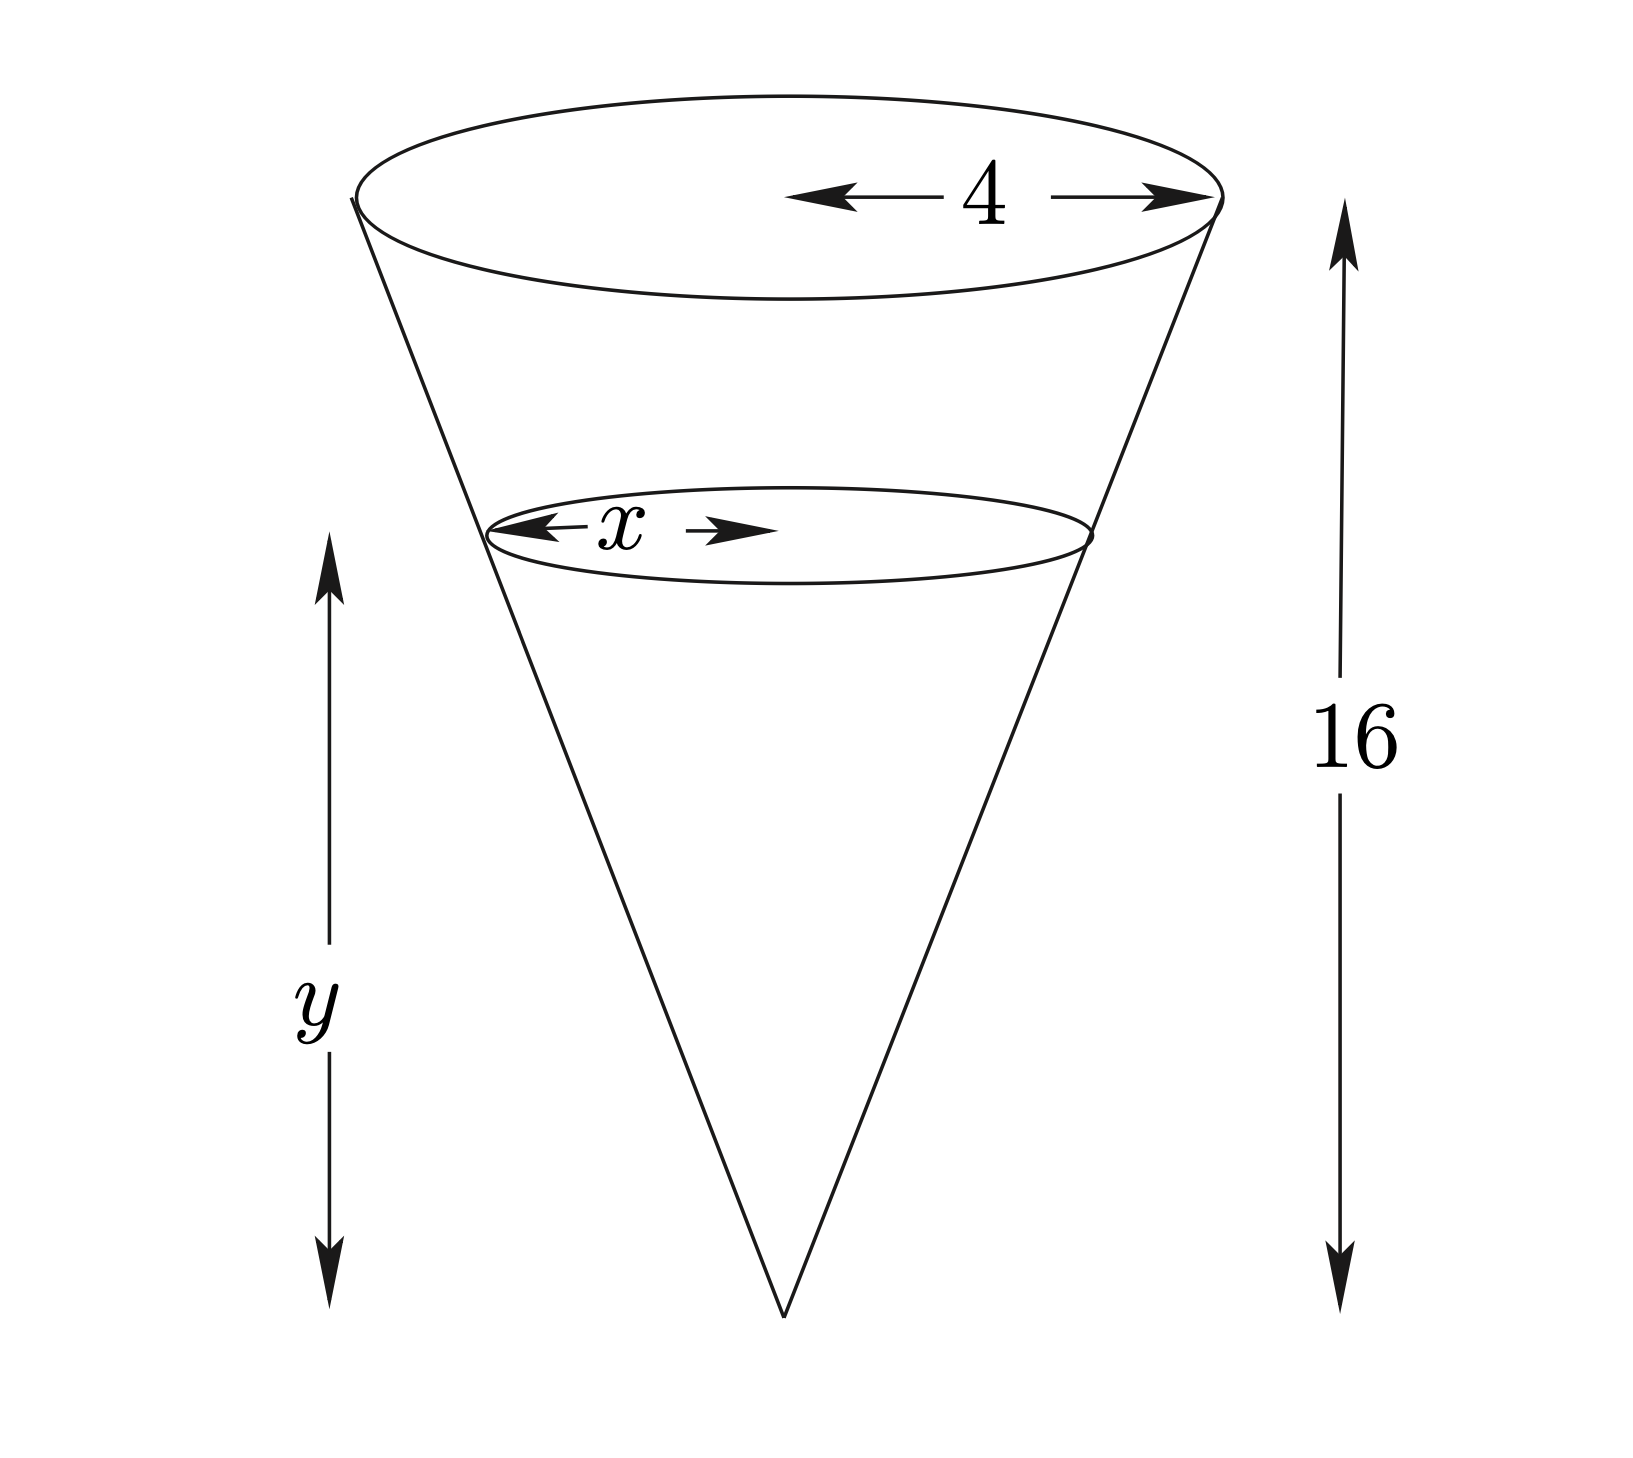
\includegraphics[width=0.5\linewidth]{images/fig-derivative-4} 

}

\caption{การไหลเวียนของอากาศในหลอดลม}\label{fig:fig-derivative-4}
\end{figure}

กำหนดให้ \(t\) เป็นเวลานับจากการเริ่มต้นการสังเกต (min) \(V\) เป็นปริมาตรของน้ำในกรวย
ณ เวลา \(t\) (in\(^3\)) \(y\) เป็นความลึกของน้ำในกรวย ณ เวลา \(t\) (in) \(x\)
เป็นรัศมีของพื้นที่ผิวของน้ำ ณ เวลา \(t\) (in) อัตราการเปลี่ยนแปลงปริมาตรของน้ำ คือ
\(\displaystyle \frac{dV}{dt}\) และ อัตราการเปลี่ยนแปลงความลึกของน้ำ คือ
\(\displaystyle  \frac{dy}{dt}\) โจทย์กล่าวว่าน้ำไหลออกจากกรวยด้วยอัตราเร็ว 2
in\(^3\)/min เมื่อระดับน้ำสูง 8 in แสดงว่า น้ำในกรวยมีปริมาตรลดลง
\[\frac{dV}{dt}\bigg{|}_{y=8} = -2\] การระบุอัตราการเปลี่ยนแปลงแบบนี้
แสดงให้เห็นว่า ณ ความลึกของน้ำต่างกัน อัตราการเปลี่ยนแปลงปริมาตรของน้ำก็จะแตกต่างกันไป
ไม่ได้เปลี่ยนแปลงด้วยอัตราที่คงที่เหมือนตัวอย่างก่อนหน้านี้
โจทย์ต้องการทราบว่าอัตราการเปลี่ยนแปลงความลึกของน้ำ เมื่อระดับน้ำสูง 8 นิ้ว นั่นคือ
\(\displaystyle  \frac{dy}{dt}\bigg{|}_{y=8}\)

จากสูตรการหาปริมาตรของกรวย \[V=\frac{1}{3}\pi x^2 y\]
และจากคุณสมบัติของสามเหลี่ยมคล้าย \(\displaystyle \frac{x}{y}=\frac{4}{16}\) หรือ
\(\displaystyle x=\frac{y}{4}\) ทำให้ได้
\(\displaystyle V=\frac{\pi}{48} y^3\) หาอนุพันธ์เทียบ \(t\) ทั้ง 2 ข้าง จะได้
\(\displaystyle \frac{dV}{dt}=\frac{\pi}{48} (3y^2 \frac{dy}{dt})\) หรือ
\(\displaystyle \frac{dy}{dt}=\frac{16}{\pi y^2} \frac{dV}{dt}\) ดังนั้น
\[\displaystyle \frac{dy}{dt}\bigg{|}_{y=8} = \frac{16(-2)}{\pi(8)^2} = \frac{-1}{2\pi} \text{ (in/min)}\]
สรุปว่า เมื่อระดับน้ำสูง 8 นิ้ว ความลึกของน้ำจะลดลงด้วยอัตรา
\(\displaystyle \frac{1}{2\pi}\) นิ้วต่อวินาที

\begin{example}
เมื่อโยนก้อนหินลงในสระน้ำ จะเกิดคลื่นซึ่งรัศมีเพิ่มขึ้นด้วย อัตรา 0.9 เมตร/วินาที
พื้นที่ที่ล้อมรอบไปด้วยคลื่นหลังจาก ผ่านไป 10 วินาทีเพิ่มขึ้นด้วยอัตราเท่าใด?
\end{example}

\textbf{วิธีทำ} กำหนดให้

\begin{enumerate}
\def\labelenumi{\arabic{enumi}.}
\item
  \(t\) แทนเวลา (วินาที)
\item
  \(r\) แทนรัศมีของคลื่น (เมตร)
\item
  \(A\) แทนพื้นที่ที่ล้อมรอบไปด้วยคลื่น (ตารางเมตร)
\end{enumerate}

พื้นที่ที่ล้อมรอบไปด้วยคลื่นเป็นไปตามสูตร \[A = \pi r^2\] เราหา derivative
เทียบกับเวลา ได้ว่า \[\frac{dA}{dt} = 2\pi r\frac{dr}{dt}\] เรามีข้อมูลว่า
\(\frac{dr}{dt} = 0.9\) เมตร ในขณะที่วินาที ที่ \(10\) รัศมีของคลื่นจึงมีค่าเท่ากับ
\(0.9\cdot 10 = 9\) เมตร และดังนั้นพื้นที่ที่ล้อมรอบไปด้วยคลื่นจึงเพิ่มขึ้นด้วยอัตรา
\[\frac{dA}{dt} = (2\pi)(9)(0.9) = 50.89\] ตารางเมตรต่อวินาที

\begin{example}
เครื่องเททราย เททรายเป็นรูปกรวย ซึ่งความสูงของกองทรายมีค่าเท่ากับ
เส้นผ่านศูนย์กลางที่ฐานของกองทรายเสมอ ถ้าความสูงเพิ่มขึ้นด้วยอัตราคงที่ 1.5 เมตร ต่อนาที
จงหาว่าเครื่องเททรายเททรายด้วยอัตราเท่าใดเมื่อกองทรายมีความ สูงเท่ากับ 3 เมตร
\end{example}

\textbf{วิธีทำ} กำหนดให้

\begin{enumerate}
\def\labelenumi{\arabic{enumi}.}
\item
  \(t\) แทนเวลา (นาที)
\item
  \(V\) แทนปริมาตรของกองทราย ณ เวลา \(t\) (ลูกบาศก์เมตร)
\item
  \(h\) แทนความสูงของกองทราย ณ เวลา \(t\) (เมตร)
\item
  \(r\) แทนรัศมีของพื้นกองทราย ณ เวลา \(t\) (เมตร)
\end{enumerate}

ในแต่ละเวลา \(t\) อัตราการเปลี่ยนแปลงของปริมาตรทรายคือ \(dV/dt\)
และอัตราการเปลี่ยนแปลงของความสูงของกองทรายคือ \(dh/dt\) จากข้อมูล ที่ให้มา เรารู้ว่า
\[\frac{dh}{dt} = 1.5\] เนื่องจากกองทรายมีลักษณะเป็นรูปกรวย ซึ่งมีสูตรว่า
\[V = \frac{1}{3}\pi r^2h\] เรายังทราบอีกว่า ที่แต่ละเวลา \(t\) ความสูงของกองทราย
มีค่าเท่ากับรัศมีของพื้นกองทราย \(r=h\) เพราะฉะนั้น \[V = \frac{1}{3}\pi h^3\] หา
derivative เทียบกับ \(t\) ได้ว่า \[\frac{dV}{dt} = \pi h^2\frac{dh}{dt}\] ดังนั้น
\[\frac{dV}{dt} = 1.5\pi h^2\] เมื่อกองทรายสูง 3 เมตร
อัตราการเปลี่ยนแปลงของปริมาตรกองทรายจึงเป็น
\[\frac{dV}{dt} = 13.5\pi = 42.41\] ลูกบาศก์เมตรต่อนาที

\begin{example}
จุด P เคลื่อนที่ไปตามเส้นโค้งตามสมการ \[y = \sqrt{x^2+16}\] เมื่อ \(P = (3,5)\) แล้ว
\(y\) มีค่าเพิ่มขึ้นด้วยอัตรา 2 หน่วย/วินาที ค่า \(x\) มีการเปลี่ยนแปลงด้วยอัตราเท่าใด
\end{example}

\textbf{วิธีทำ} กำหนดให้

\begin{enumerate}
\def\labelenumi{\arabic{enumi}.}
\tightlist
\item
  \(t\) แทนเวลา (วินาที)
\end{enumerate}

เราหา derivative ของสมการที่กำหนดเทียบกับเวลา \(t\) พบว่า \[\label{E:example}
    \frac{dy}{dt} = \frac{x}{\sqrt{x^2+16}}\frac{dx}{dt}\] เรารู้ว่าที่จุด
\(P = (3,5)\) \[\frac{dy}{dt} = 2\]
แทนค่าทั้งสองในสมการ~\hyperref[E:example]{\[E:example\]} เราจะได้ว่า
\[2 = \frac{2}{\sqrt{9+16}}\frac{dx}{dt}\] นั่นคือ \[\frac{dx}{dt} = 5\]
นั่นคือ \(x\) มีการเปลี่ยนแปลงด้วยอัตรา 5 หน่วยต่อวินาที

\begin{example}
ท่าเรือหนึ่ง มีแท่งแขวนลูกรอกผูกเรืออยู่เหนือท่า มีเชือกผูกไว้กับ
หัวเรือซึ่งอยู่ต่ำกว่าตัวรอกของแท่งแขวน 3 เมตร ถ้าเราดึงเชือกด้วยอัตราเร็ว 6 เมตร/นาที
เรือถูกดึงเข้าหาท่าด้วยอัตราเร็วเท่าใดเมื่อเชือก จากหัวเรือถึงลูกรอกมีความยาว 40 เมตร
\end{example}

\textbf{วิธีทำ} กำหนดให้

\begin{enumerate}
\def\labelenumi{\arabic{enumi}.}
\item
  \(t\) แทนเวลา (นาที)
\item
  \(x\) ระยะทางในแนวนอน (เมตร)
\item
  \(y\) ระยะทางในแนวดิ่ง (เมตร)
\end{enumerate}

จากข้อมูลของปัญหา เราสรูปได้ว่า อัตราการดึงเชือกแทนด้วยพจน์ \[\frac{dy}{dt} = 6\]
คำถามให้ \(\frac{dx}{dt}\) เมื่อเชือกยาว 40 เมตรนับจากหัวเรือถึงลูกรอก
โดยการใช้พิทาโกรัส เราจึงได้ความสัมพันธ์ \[x^2+y^2 = 40^2\] เราหา derivative
เทียบกับ \(t\) ทั้งสองข้างของสมการ \begin{equation}   \begin{aligned}
    2x \frac{dx}{dt} + 2y\frac{dy}{dt} &= 0 \\
    x \frac{dx}{dt} + y\frac{dy}{dt} &= 0
  \end{aligned} \end{equation} เนื่องจากลูกรอกอยู่สูงกว่าหัวเรือ 3 เมตร หรือ \(y=3\)
ในขณะที่ การดึงเชือกด้วยอัตราเร็ว 6 เมตร หรือ \(\frac{dy}{dt} = 6\) เพราะฉะนั้น
เมื่อเชือกยาว 40 เมตร เรืออยู่ห่างออกไปเป็นระยะทาง \[x^2 + 3^2 = 40^2\] หรือ
\(x = \sqrt{1591}\) ดังนั้น \begin{equation}   \begin{aligned}
    \sqrt{1591}\frac{dx}{dt} + 4(6) &= 0 \\
    \frac{dx}{dt} &= -\frac{24}{\sqrt{1591}} = -0.60
  \end{aligned} \end{equation} ซึ่งหมายถึงเรือถูกดึงเข้าหาท่าด้วยอัตราเร็ว 0.6
เมตรต่อนาที

\begin{enumerate}
\def\labelenumi{\arabic{enumi}.}
\item
  วาดภาพและกำหนดตัวแปรต่างๆ เช่น \(x\), \(y\) เป็นต้น
\item
  ระบุอัตราการเปลี่ยนแปลงของตัวแปรทุกตัวที่โจทย์กำหนดให้ และที่โจทย์ต้องการให้หา เช่น
  \(\displaystyle\frac{dx}{dt}\), \(\displaystyle\frac{dy}{dt}\) เป็นต้น
\item
  หาสมการสมการหนึ่งที่แสดงให้เห็นถึงความสัมพันธ์ระหว่างตัวแปรที่กำหนดขึ้นในขั้นตอนที่ 1
  และเมื่อหาอนุพันธ์ของสมการนี้ จะมีเทอมที่เกี่ยวข้องกับอนุพันธ์ในขั้นตอนที่ 2
\item
  หาอนุพันธ์ทั้ง 2 ข้างของสมการในขั้นตอนที่ 3
  เทียบกับเวลาและนำค่าของอนุพันธ์ที่ทราบลงไปในสมการ
\item
  หาค่าของอนุพันธ์ที่โจทย์ต้องการด้วยวิธีทางพีชคณิต
\end{enumerate}

\subsection{แบบฝึกหัด}\label{uxe41uxe1auxe1auxe1duxe01uxe2buxe14-2}

\begin{enumerate}
\def\labelenumi{\arabic{enumi}.}
\item
  กำหนดให้ \(y= \ln x\) จงหา \(dy\) และ \(\Delta y\) ที่ \(x=1\) โดย ที่
  \(dx = \Delta x = 0.5\)
\item
  พิจารณาฟังก์ชันต่อไปนี้ แล้วหาสูตร \(dy\) และ \(\Delta y\)

  \begin{enumerate}
  \def\labelenumii{\arabic{enumii}.}
  \item
    \(\displaystyle y = x\sqrt{x-1}\)
  \item
    \(\displaystyle y = xe^x\)
  \item
    \(\displaystyle y = x\sin  x\)
  \item
    \(\displaystyle y = \tan (x^2)\)
  \end{enumerate}
\item
  จงหา local linear approximation ของเส้นโค้งจากสมการ \(xe^y = y\) ที่จุด
  \((0,0)\) และใช้สมการที่ได้ประมาณค่าของ \(y\) เมื่อ \(x=0.1\)
\item
  จงหา \(\frac{dy}{dx}\) สำหรับความสัมพันธ์ต่อไปนี้

  \begin{enumerate}
  \def\labelenumii{\arabic{enumii}.}
  \item
    \(x^2+ y^2 = 25\)
  \item
    \(\frac{1}{x} + \frac{1}{y} = 1\)
  \item
    \(x\sin y + y\sin x = 1\)
  \item
    \(e^{xy} + xy = 1\)
  \end{enumerate}
\item
  หญิงคนหนึ่งสูง 1.55 เมตร เดินเข้าเสาไฟด้วยอัตราเร็ว 0.75 เมตร/วินาที
  เสาไฟติดดวงไฟสูง 5 เมตร

  \begin{enumerate}
  \def\labelenumii{\arabic{enumii}.}
  \item
    เงาของหญิงคนนี้เปลี่ยนแปลงด้วยอัตราเท่าใด
  \item
    ปลายเงาของด้านศรีษะหญิงคนนี้เคลื่อนที่ด้วยอัตราเร็วเท่าใด
  \end{enumerate}
\item
  อนุภาคหนึ่งเคลื่อนที่ไปตามเส้นโค้งอธิบายตามสมการ
  \[\frac{x^2y}{1+y^2} = \frac{2}{5}\] กำหนดให้พิกัดแกน \(x\)
  ของอนุภาคเพิ่มขึ้นด้วยอัตรา 4 หน่วย/วินาที เมื่ออนุภาคอยู่ที่ตำแหน่ง \((1,2)\)

  \begin{enumerate}
  \def\labelenumii{\arabic{enumii}.}
  \item
    พิกัดแกน \(y\) ของอนุภาคเปลี่ยนแปลงด้วยอัตราเท่าใด เมื่ออนุภาคอยู่ที่ตำแหน่ง
    \((1,2)\)
  \item
    ณ ตำแหน่ง \((1,2)\) อนุภาคกำลังเคลื่อนสูงขึ้นหรือลดลงในพิกัด \(xy\)
  \end{enumerate}
\item
  ความเข้มของแสงที่ผ่านเข้าตาขึ้นอยู่กับรัศมีของ pupil ถ้า pupil มีขนาดมากขึ้น
  ปริมาณของแสงก็จะเข้าตามากขึ้น ดังสมการ \(I=kr^2\) เมื่อ \(I\) เป็นความเข้มของแสง
  \(r\) เป็นรัศมีของ pupil และ \(k\) เป็นค่าคงตัว ในช่วงเวลา 6 โมงเช้าถึงเที่ยง
  รัศมีของ pupil จะขยายตัวด้วยอัตราเร็วคงที่ 0.1 mm/min จงหาว่าในช่วงเวลาดังกล่าว
  ความเข้มของแสงที่ผ่านเข้าตา จะมีการเปลี่ยนแปลงอย่างไร เมื่อ \(r=0.5\) cm
\item
  การแพร่ระบาดของแมลงวันทอง เริ่มที่ใจกลางของหมู่บ้านเล็กๆ แห่งหนึ่งนอกเมือง
  พื้นที่การแพร่ระบาดมีลักษณะคล้ายวงกลมดังแสดงในรูป
  \hyperref[fig-fly]{1.5}
  รัศมีของพื้นที่การแพร่ระบาดขยายเพิ่มขึ้นด้วยอัตรา 1.5 ไมล์ต่อปี
  จงหาอัตราการเปลี่ยนแปลงของพื้นที่การแพร่ระบาด เมื่อรัศมีของพื้นที่การแพร่บาดมีค่าเท่ากับ
  4 ไมล์
\end{enumerate}

\begin{figure}

{\centering 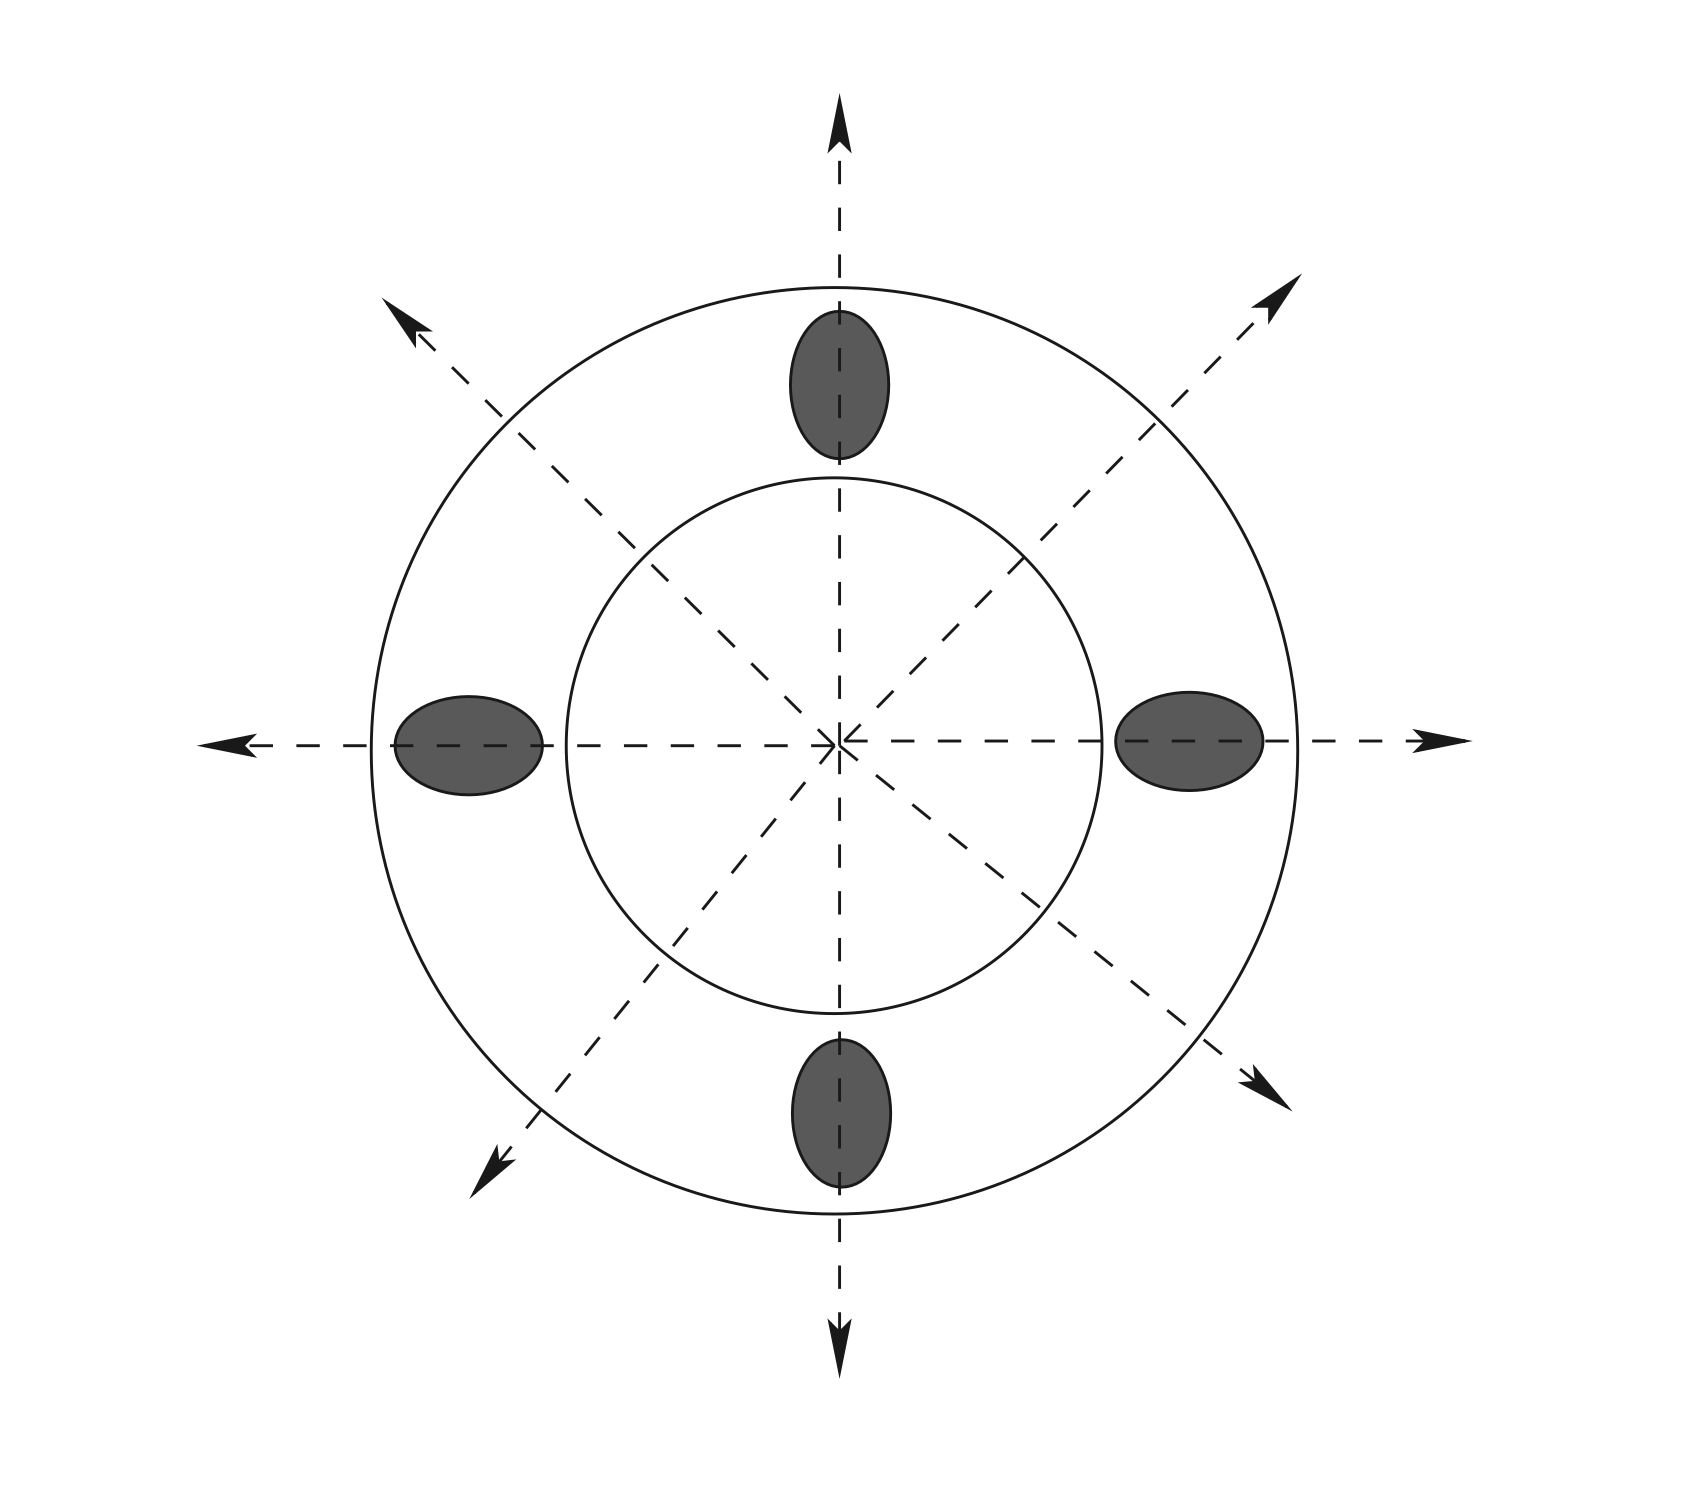
\includegraphics[width=0.5\linewidth]{images/fig-derivative-5} 

}

\caption{การแพร่ระบาดของแมลงวันทอง โดยที่วงรีสีเทาแทนแมลงวัน}\label{fig:fig-derivative-5}
\end{figure}

\section{อนุพันธ์ของฟังก์ชันตรีโกณมิติและอินเวอร์สของฟังก์ชันตรีโกณมิติ}\label{uxe2duxe19uxe1euxe19uxe18uxe02uxe2duxe07uxe1fuxe07uxe01uxe0auxe19uxe15uxe23uxe42uxe01uxe13uxe21uxe15uxe41uxe25uxe30uxe2duxe19uxe40uxe27uxe2duxe23uxe2auxe02uxe2duxe07uxe1fuxe07uxe01uxe0auxe19uxe15uxe23uxe42uxe01uxe13uxe21uxe15}

\subsection{อนุพันธ์ของฟังก์ชันตรีโกณมิติ}\label{uxe2duxe19uxe1euxe19uxe18uxe02uxe2duxe07uxe1fuxe07uxe01uxe0auxe19uxe15uxe23uxe42uxe01uxe13uxe21uxe15}

เราจะใช้ความรู้เกี่ยวกับเอกลักษณ์ตรีโกณมิติและลิมิตของฟังก์ชันตรีโกณ
ช่วยในการหาอนุพันธ์ของฟังก์ชันตรีโกณมิติโดยนิยามดังนี้\\
\begin{equation}   \begin{aligned}
 \lim_{x\rightarrow 0} \frac{\sin x}{x}    &= 1  \quad \text{ เมื่อ x มีหน่วยเป็นเรเดียน }\\
 \lim_{x\rightarrow 0} \frac{\cos x -1}{x} &= 1  \\
    \sin A- \sin B                         &=2 \cos \frac{A+B}{2}\sin \frac{A-B}{2}
  \end{aligned} \end{equation}

\begin{theorem}
ถ้า \(f(x)=\sin x\) แล้ว \(\displaystyle \frac{d}{dx}\sin x =\cos x\)
\end{theorem}

\begin{equation}   \begin{aligned}
\displaystyle \frac{d}{dx}\sin x&=\lim_{h\rightarrow 0}(\frac{\sin
(x+h)-\sin x}{h})\\
\displaystyle  &=\lim_{h\rightarrow0} \frac{2\cos
(x+\frac{h}{2})\sin \frac{h}{2}}{h}\\
\displaystyle &=2\lim_{h\rightarrow 0}\cos
(x+\frac{h}{2}).\lim_{h\rightarrow 0} \frac{\sin \frac{h}{2}}{h}\\
\displaystyle &=2\cos x\lim_{\frac{h}{2} \rightarrow 0}\frac{\frac{1}{2}\sin
\frac{h}{2}}{\frac{h}{2}}\\
\displaystyle &=2(\cos x)\frac{1}{2}\\
&=\cos x
  \end{aligned} \end{equation}

เนื่องจาก \begin{equation}   \begin{aligned}
 \sin (x+h)- \sin x &=2\cos \frac{x+h+x}{2}\sin \frac{h}{2}\\
                        &=2\cos (x+\frac{h}{2})\sin \frac{h}{2}
  \end{aligned} \end{equation}

\hfill\break
สำหรับการหาอนุพันธ์ของ cosine ก็ทำได้ในทำนองเดียวกันกับ sine ส่วนฟังก์ชันตรีโกณมิติอื่นๆ
หาได้โดยแปลงในรูป cosine หรือ sine เช่น

\[\tan x= \frac{\sin x}{\cos x}, \quad \cot x=\frac{\cos x}{\sin
x}, \quad \sec x=\frac{1}{\cos x} \text{ และ } \displaystyle \csc x=\frac{1}{\sin x}\]

\begin{theorem}
\leavevmode

\begin{enumerate}
\def\labelenumi{\arabic{enumi}.}
\item
  \(\displaystyle\frac{d}{dx}\cos x=-\sin x\)
\item
  \(\displaystyle\frac{d}{dx}\tan x=\sec^{2} x\)
\item
  \(\displaystyle\frac{d}{dx}\cot x=-\csc^{2} x\)
\item
  \(\displaystyle\frac{d}{dx}\sec x=\sec x \tan x\)
\item
  \(\displaystyle\frac{d}{dx}\csc x=-\csc x\cot x\)
\end{enumerate}

\end{theorem}

\begin{equation}   \begin{aligned}
\displaystyle \frac{d}{dx}\sec x&=\frac{d}{dx}.\frac{1}{\cos x}\\
&=\frac{d}{dx}(\cos x)^{-1}\\
&=(-1)(\cos x)^{-2}\displaystyle \frac{d}{dx}\cos x\\
&=\displaystyle \frac{-1}{\cos^{2} x}(-\sin x)\\
&=\displaystyle \frac{1}{\cos x}.\frac{\sin x}{\cos x}\\
&=\sec x\tan x
  \end{aligned} \end{equation}

\begin{example}
กำหนดให้ \(y=x^{2}\tan 3x\) จงหา \(\displaystyle
\frac{dy}{dx}\)
\end{example}

\textbf{วิธีทำ} \begin{equation}   \begin{aligned}
\displaystyle \frac{dy}{dx}&=\frac{d}{dx}(x^{3}\tan 3x)\\
&=x^{2}\displaystyle \frac{d}{dx}\tan 3x+\tan 3x\frac{d}{dx}x^{2}\\
&=x^{2}(\sec^{2}3x)(3)+(\tan 3x)(2x)\\
&=3x^{2}\sec^{2}3x+2x\tan 3x
  \end{aligned} \end{equation}

\begin{example}
กำหนดให้ \(\displaystyle y=\frac{\sin x}{1+\cos x}\) จงหา
\(\displaystyle \frac{dy}{dx}\)
\end{example}

\textbf{วิธีทำ} \begin{equation}   \begin{aligned}
\displaystyle \frac{dy}{dx}&=\frac{d}{dx}(\frac{\sin x}{1+\cos x})\\
&=\frac{(1+\cos x)\displaystyle \frac{d}{dx}\sin x -\sin x\displaystyle
\frac{d}{dx}(1+\cos x)}{(1+\cos x)^{2}}\\
&=\frac{(1+\cos x)\cos x-(\sin x)(-\sin x)}{(1+\cos x)^{2}}\\
&=\frac{\cos x+\cos^{2}x+\sin^{2}x }{(1+\cos x)^{2}}\\
&=\frac{\cos x+1}{(1+\cos x)^{2}}\\
&=\frac{1}{1+\cos x}
  \end{aligned} \end{equation}

\begin{example}
กำหนดให้ \(y=\sec^{2}(3x-1)\) จงหา \(\displaystyle
\frac{dy}{dx}\)
\end{example}

\textbf{วิธีทำ} \begin{equation}   \begin{aligned}
\displaystyle \frac{dy}{dx}&=\frac{d}{dx}\sec^{2}(3x-1)\\
&=2\sec(3x-1)\displaystyle \frac{d}{dx}\sec(3x-1)\\
&=2\sec(3x-1)\sec(3x-1)\tan(3x-1)\displaystyle \frac{d}{dx}(3x-1)\\
&=3.2\sec^{2}(3x-1)\tan(3x-1)\\
&=6\sec^{2}(3x-1)\tan(3x-1)
  \end{aligned} \end{equation}

\begin{example}
ถ้า \(x\cos y+y\cos x=1\) จงหา \(\displaystyle \frac{dy}{dx}\)
\end{example}

\textbf{วิธีทำ} ใช้ implicit differentiation \begin{equation}   \begin{aligned}
\displaystyle \frac{d}{dx}(x\cos y +y\cos x)&=\frac{d}{dx}1\\
\displaystyle \frac{d}{dx}(x\cos y)+\frac{d}{dx}(y\cos x)&=0\\
\displaystyle x\frac{d}{dx}\cos y+\cos y \frac{dx}{dy}+y\frac{d}{dx}\cos
x+\cos x\frac{dy}{dx}&=0\\
\displaystyle x(-\sin y)\frac{dy}{dx}+\cos y + y(-\sin x)+\cos
x\frac{dy}{dx}&=0\\
\displaystyle (-x\sin y+\cos x)\frac{dy}{dx}&=y\sin x -\cos y\\
\displaystyle \frac{dy}{dx}&=\frac{y\sin x-\cos y}{\cos x-x\sin y}
  \end{aligned} \end{equation}

\begin{example}
จงหา \(\displaystyle \frac{d^{2}y}{dx^{2}}\) ของฟังก์ชัน \(y=
x\cos x\)
\end{example}

\textbf{วิธีทำ} \begin{equation}   \begin{aligned}
y&= x\cos x\\
\displaystyle y'&=\frac{d}{dx}(x\cos x)\\
&=\displaystyle \frac{d}{dx}\cos x +\cos x\frac{dx}{dx}\\
&=-x\sin x + \cos x\\
\displaystyle y''&=-(x\frac{d}{dx}\sin x + \sin x\frac{dx}{dx}) +
\frac{d}{dx}\cos x \\
&=-(x\cos x + \sin x)-\sin x\\
&=-x\cos x - 2\sin x
  \end{aligned} \end{equation}

\subsection{อนุพันธ์ของฟังก์ชันอินเวอร์สของฟังก์ชันตรีโกณมิติ}\label{uxe2duxe19uxe1euxe19uxe18uxe02uxe2duxe07uxe1fuxe07uxe01uxe0auxe19uxe2duxe19uxe40uxe27uxe2duxe23uxe2auxe02uxe2duxe07uxe1fuxe07uxe01uxe0auxe19uxe15uxe23uxe42uxe01uxe13uxe21uxe15}

จะเห็นว่าฟังก์ชันตรีโกณมิติทั้งหมดคือ sine, cosine, tangent, cotangent, secant และ
cosecant เป็นฟังก์ชันคาบซึ่งสมาชิกในโดเมน จะให้ค่าซ้ำกัน ดังนั้น ฟังก์ชันตรีโกณมิติจึงไม่เป็น
1-1 ฟังก์ชัน แต่เราสามารถจำกัดโดเมนของฟังก์ชันตรีโกณมิติเพื่อทำให้ฟังก์ชันเหล่านี้ เป็น 1-1
ฟังก์ชัน ก็จะทำให้อินเวอร์สของฟังก์ชันเหล่านั้นเป้นฟังก์ชันด้วย เช่น
\[F=\{(x,y)|y=\sin x\} \text{ มีโดเมน }=\Re \text { และเรนจ์ }=[-1,1]\]
ไม่เป็น1-1ฟังก์ชัน แต่
\[F=\{(x,y)|y=\sin x , x\in \displaystyle [-\frac{\pi}{2},\frac{\pi}{2}]\}\]
เป็น 1-1 ฟังก์ชัน ดังนั้น
\[F^{-1}=\{(x,y)|x=\sin y , y\in \displaystyle [-\frac{\pi}{2},\frac{\pi}{2}],
x\in [-1,1]\}\] เป็น อินเวอร์สฟังก์ชันของ\(F\)เรียกว่า inverse sine function
ใช้สัญลักษณ์ \(\sin^{-1} x\) หรือ \(\arcsin x\)

ในทำนองเดียวกัน

\begin{theorem}
\leavevmode

\begin{enumerate}
\def\labelenumi{\arabic{enumi}.}
\item
  \(\displaystyle\frac{d}{dx} \arcsin x=\frac{1}{\sqrt{1-x^{2}}}., |x|<1\)
\item
  \(\displaystyle\frac{d}{dx} \arccos x=\frac{-1}{\sqrt{1-x^{2}}}., |x|<1\)
\item
  \(\displaystyle\frac{d}{dx} arccot x=\frac{-1}{1+x^{2}}.\)
\item
  \(\displaystyle\frac{d}{dx} arcsec x=\frac{1}{|x|\sqrt{x^{2}-1}}, |x|>1\)
\item
  \(\displaystyle\frac{d}{dx} arccosec x=\frac{-1}{|x|\sqrt{x^{2}-1}}, |x|>1\)
\item
  \(\displaystyle\frac{d}{dx} \arctan x=\frac{1}{1+x^{2}}\)
\end{enumerate}

\end{theorem}

ให้ \(y=\arcsin x , |x|<1\)\\
\begin{equation}   \begin{aligned}
x&=\sin y, \displaystyle \frac{-\pi}{2}\leq y \leq \frac{\pi}{2}\\
\displaystyle \frac{dx}{dx}&=\frac{d}{dx}\sin y\\
1&=\cos y \displaystyle \frac{dy}{dx}\\
\displaystyle \frac{dy}{dx}&=\frac{1}{\cos y} , |x|<1\\
&=\displaystyle \frac{1}{\sqrt{1-\sin^{2} y}}\\
&=\displaystyle \frac{1}{\sqrt{1-x^{2}}}
  \end{aligned} \end{equation}

\begin{example}
จงหา \(\displaystyle \frac{dy}{dx}\) เมื่อ \(y=\sin^{-1}(2x)\)
\end{example}

\textbf{วิธีทำ} \begin{equation}   \begin{aligned}
 \displaystyle
\frac{dy}{dx}&=\frac{1}{\sqrt{1-(2x)^{2}}}.\frac{d}{dx}(2x)\\
&=\frac{2}{\sqrt{1-4x^{2}}}
  \end{aligned} \end{equation}

\begin{example}
จงหา \(y'\) เมื่อ \(y=arcsec x^{2}\)
\end{example}

\textbf{วิธีทำ} \begin{equation}   \begin{aligned}
 \displaystyle y'&=\frac{d}{dx}arcsec
x^{2}\\
&=\displaystyle \frac{1}{|x|^{2}\sqrt{x^{4}-1}}.\frac{d}{dx}(x)^{2}\\
&=\displaystyle \frac{2x}{x^{2}\sqrt{x^{4}-1}}\\
&=\displaystyle \frac{2}{x\sqrt{x^{4}-1}}
  \end{aligned} \end{equation}

\begin{example}
จงหา \(y'\) เมื่อ \(y=cot^{-1}\displaystyle(\frac{1}{x})-\tan^{-1}x\)
\end{example}

\textbf{วิธีทำ} \begin{equation}   \begin{aligned}
\displaystyle y&=\cot^{-1}(\frac{1}{x})-\tan^{-1}\\
\displaystyle y'&=\frac{d}{dx}(\cot^{-1}(\frac{1}{x})-\tan^{-1})\\
\displaystyle &=\frac{d}{dx}\cot^{-1}(\displaystyle
\frac{1}{x})-\frac{d}{dx}\tan^{-1}x\\
\displaystyle &=\frac{-1}{1-\displaystyle
\frac{1}{x^{2}}}(-\frac{1}{x^{2}})-\frac{1}{1+x^{2}}\\
\displaystyle &=\frac{1}{x^{2}-1}-\frac{1}{1+x^{2}}\\
\displaystyle &=\frac{2}{x^{4}-1}
  \end{aligned} \end{equation}

\chapter{การประยุกต์ของอนุพันธ์ (Applications of Differentiation)}\label{uxe01uxe32uxe23uxe1buxe23uxe30uxe22uxe01uxe15uxe02uxe2duxe07uxe2duxe19uxe1euxe19uxe18-applications-of-differentiation}

\section{Applications of derivatives related to students discipline}\label{applications-of-derivatives-related-to-students-discipline}

จากบทเรียนก่อนหน้านี้ เราทราบว่าถ้าตัวแปร \(y\) สามารถเขียนอธิบายได้ด้วยฟังก์ชันๆ หนึ่ง
ที่ขึ้นกับตัวแปร \(x\) นั่นคือ \(f(x)\) เราจะสามารถวาดกราฟของ \(y\) หรือฟังก์ชัน \(f(x)\) ได้
และถ้าเราทราบว่า จุด \(P(x_0,y_0)\) และจุด \(Q(x_1,y_1)\) ต่างอยู่บนกราฟของ \(y\)
แสดงว่า \(y_0=f(x_0)\) และ \(y_1=f(x_1)\) นั่นเอง ความชันของเส้นตรงที่ลากผ่านจุด \(P\)
และจุด \(Q\) มักใช้ \(m\) เป็นสัญลักษณ์ มีสูตรการหาดังนี้
\[m=\frac{\triangle y}{\triangle x}=\frac{y_1-y_0}{ x_1-x_0}=\frac{f(x_1)-f(x_0)}{ x_1-x_0}=\frac{y_0-y_1}{ x_0-x_1}\]
ความชันของเส้นตรงที่กล่าวมาแล้วนี้ มีชื่อเรียกอีกชื่อหนึ่งว่า อัตราการเปลี่ยนแปลงเฉลี่ยของ
\(f(x)\) ตั้งแต่ \(x=x_0\) จนถึง \(x=x_1\) และ
\[\lim_{x_1 \rightarrow x_0} \frac{f(x_1)-f(x_0)}{ x_1-x_0} =f'(x_0)\]
คืออัตราการเปลี่ยนแปลงของ \(f(x)\) ณ \(x=x_0\) หรือการหาอนุพันธ์ของฟังก์ชัน \(f(x)\)
เทียบกับตัวแปร \(x\) เมื่อ \(x\) มีค่าเท่ากับ \(x_0\) นั่นเอง

หลักการหาอนุพันธ์สามารถนำไปประยุกต์ใช้ได้ในหลากหลายสาขาวิชาชีพ ไม่ว่าจะเป็นธุรกิจ
เศรษฐศาสตร์ วิศวกรรมศาสตร์ ฟิสิกส์ เคมี หรือแม้กระทั่งชีววิทยา สำหรับบทนี้
ผู้เขียนจะขอกล่าวถึง การนำแนวคิดทางคณิตศาสตร์นี้ไปประยุกต์ใช้กับปัญหาทางวิทยาศาสตร์ชีวภาพ
เพื่อให้สอดคล้องกับความสนใจของผู้เรียน

\begin{example}
AIDS ย่อมาจาก acquired immunodeficiency syndrome
เป็นโรคติดต่อทางเพศสัมพันธ์และการให้เลือด ซึ่งพบการแพร่ระบาดมาตั้งแต่ปี พ.ศ. 2523
โดยผู้ป่วยที่เป็นโรค AIDS จะพบเชื้อไวรัส HIV ใน antibodies ซึ่งไวรัส HIV
นี้มีระยะฟักตัวตั้งแต่ไม่กี่เดือน จนกระทั่งนานนับปี นักวิจัยคนหนึ่งนำเชื้อไวรัส HIV
มาเพาะเลี้ยงในจานเพาะเชื้อ พบว่า ขนาดของประชากรไวรัส ณ เวลา \(t\) , \(N(t)\)
สอดคล้องกับสมการ \(N(t)=1000+20t+t^2\) อยากทราบว่าไวรัสชุดนี้มีอัตราการเปลี่ยนแปลง ณ
\(t\) ใดๆ เป็นอย่างไร
\end{example}

กำหนดให้ \(t\) แทน เวลา \(N(t)\) แทน ขนาดของประชากรไวรัส ณ เวลา \(t\)
จากการทดลองพบว่า ขนาดของประชากรไวรัส ณ เวลา \(t\) ใดๆ สอดคล้องกับสมการ
\[N(t)=1000+20t+t^2\] ดังนั้น อัตราการเปลี่ยนแปลงของขนาดของประชากรไวรัส ณ เวลา
\(t\) ใดๆ คือ \[\frac{dN}{dt}=20+2t\]

\begin{example}
จากการสำรวจพบว่า จำนวนผู้ป่วยด้วยโรค AIDS, \(P(t)\) มีความสัมพันธ์กับสมการ
\[P(t)=100t^2-2t^3\] เมื่อ \(t\) เป็นเวลาที่ผ่านไปนับจากวันนี้ มีหน่วยเป็นวัน
อยากทราบว่าเมื่อ 20 วันผ่านไป จะมีผู้ป่วยด้วยโรคนี้กี่คน
และมีอัตราการเพิ่มจำนวนผู้ป่วยเป็นเท่าไหร่
\end{example}

กำหนดให้ \(t\) แทน เวลา มีหน่วยเป็นวัน \(P(t)\) แทน จำนวนผู้ป่วยด้วยโรค AIDS
มีหน่วยเป็นคน จากการสำรวจพบว่า \[P(t)=100t^2-2t^3\] เมื่อ 20 วันผ่านไป แสดงว่า
\(t=20\) จะได้ว่า \(P(20)=100(20)^2-2(20)^3=24,000\) ดังนั้น เมื่อ 20 วันผ่านไป
จะมีผู้ป่วยโรค AIDS 24,000 คน อัตราการเพิ่มจำนวนผู้ป่วยโรค AIDS ณ เวลา \(t\) ใดๆ
หาได้ดังนี้ \[\frac{dP}{dt}=200t-6t^2\] ดังนั้น เมื่อ 20 วันผ่านไป
อัตราการเพิ่มจำนวนผู้ป่วยจะมีค่าเท่ากับ \(200(20)-6(20)^2\) หรือ \(1,600\) คนต่อวัน

\begin{example}
จากการศึกษาทางสิ่งแวดล้อมระบุว่า \(Q(t)\) ระดับ carbon monoxide (CO) เฉลี่ยในอากาศ
(หน่วยเป็น ppm) จะมีค่าเป็นเท่าไร \[Q(t)=0.05t^2+0.1t+3.4\] เมื่อ \(t\)
เป็นเวลาที่นับจากนี้เป็นต้นไป มีหน่วยเป็นปี อยากทราบว่า ระดับ CO
เฉลี่ยในอากาศจะเปลี่ยนแปลงไปอย่างไร ในอีก 2 ปี ข้างหน้า
\end{example}

กำหนดให้ \(t\) เป็นเวลาที่นับจากวันนี้ มีหน่วยเป็นปี \(Q(t)\) เป็นระดับ CO
เฉลี่ยในอากาศมีหน่วยเป็น ppm จากการศึกษาทางสิ่งแวดล้อมระบุว่า
\[Q(t)=0.05t^2+0.1t+3.4\] อัตราการเปลี่ยนแปลงระดับ CO เฉลี่ยในอากาศ ณ \(t\) ใดๆ
คือ \[\frac{dQ}{dt}=0.1t+0.1\] ในอีก 2 ปีข้างหน้า \(t=2\)
\[\frac{dQ}{dt}=0.1(2)+0.1=0.3>0\] ระดับ CO เฉลี่ยในอากาศจะเพิ่มขึ้น (เพราะ
\(\displaystyle\frac{dQ}{dt}>0\)) ด้วยอัตราเร็ว 0.3 ppm ต่อปี

\begin{example}
Poiseuille's law กล่าวว่า ความเร็วของเลือด (หน่วย คือ เซนติเมตรต่อวินาที)
ที่อยู่ห่างจากจุดกึ่งกลางของหลอดเลือด \(r\) เซนติเมตร มีสูตรดังนี้ \(S(r)=C(R^2-r^2)\) เมื่อ
\(C\) เป็นค่าบวกใดๆ และ \(R\) เป็นรัศมีของหลอดเลือด อยากทราบว่า
ความเร็วของเลือดจะเปลี่ยนแปลงเป็นอย่างไร
เมื่อเลือดอยู่บริเวณกึ่งกลางระหว่างจุดกึ่งกลางและผนังของหลอดเลือด
\end{example}

กำหนดให้ \(r\) เป็นระยะห่างจากจุดกึ่งกลางของหลอดเลือด (หน่วยเป็นเซนติเมตร) \(S(r)\)
เป็นความเร็วของเลือด ณ \(r\) ใดๆ (หน่วยเป็นเซนติเมตรต่อวินาที) จาก Poiseuille's law
\[S(r)=C(R^2-r^2)\] อัตราการเปลี่ยนแปลงความเร็วของเลือด ณ \(r\) ใดๆ คือ
\[\frac{dS}{dr}=-2Cr\]
เลือดที่อยู่บริเวณกึ่งกลางระหว่างจุดกึ่งกลางและผนังของหลอดเลือดหมายถึง \(r=\frac{R}{2}\)
ดังนั้น
\[\frac{ds}{dr}\bigg{|}_{r=R/2} =  - CR < 0 \text{ เพราะว่า } C>0, R>0\]
แสดงว่าความเร็วของเลือดจะลดลง (เพราะ \(\displaystyle\frac{dS}{dr}<0\))
ด้วยอัตรา \(CR\) (cm/s)/cm

\subsection{แบบฝึกหัด}\label{uxe41uxe1auxe1auxe1duxe01uxe2buxe14-3}

\begin{enumerate}
\def\labelenumi{\arabic{enumi}.}
\item
  ผลการทดลองแสดงให้เห็นว่า ความเข้มข้นของปริมาณ adrenaline ที่ฉีดเข้าไปในร่างกาย,
  \(x\), มีความสัมพันธ์กับการตอบสนองของกล้ามเนื้อ, \(y\), ด้วยสมการ
  \(y=\frac{x}{a+bx}\) เมื่อ \(a\) และ \(b\) เป็นค่าคงตัว
  จงหาอัตราการเปลี่ยนแปลงการตอบสนองของกล้ามเนื้อ เมื่อเทียบกับความเข้มข้นของปริมาณ
  adrenaline ที่ฉีดเข้าไปในร่างกาย
\item
  กำหนดให้ \(\displaystyle P(t)=\frac{1000t}{t+10}\)
  แสดงถึงขนาดของประชากรแบคทีเรีย เมื่อ \(t\) เป็นเวลา
  จงหาอัตราการเจริญเติบโตของประชากร
\item
  Schuty - Borisoff laws กล่าวถึง ปริมาณ substrate, \(y\),
  ที่ถูกเปลี่ยนรูปด้วยเอนไซม์ ในรูปของฟังก์ชันที่ขึ้นกับเวลา \(t\) ดังนี้ \[y=k\sqrt{cat}\]
  เมื่อ \(k\), \(a\), \(c\) เป็นค่าคงตัว จงหาอัตราการเปลี่ยนแปลงปริมาณ substrate
  ที่ถูกเปลี่ยนรูปด้วยเอนไซม์ ณ เวลา \(t\) ใดๆ
\end{enumerate}

\section{Sketching the graph of a function from the derivative}\label{sec-sketch}

ในหัวข้อนี้เราใช้ประโยชน์จากเรื่อง derivative ในการวาดกราฟของฟังก์ชัน
เมื่อนึกถึงกราฟของฟังก์ชัน เราสนใจลักษณะที่สำคัญ เช่นช่วงใดที่กราฟเพิ่ม ช่วงใดที่กราฟลด
ค่าสูงสุดและค่าต่ำสุดของกราฟอยู่ที่ใด กราฟมีลักษณะคว่ำในช่วงใด หรือมีลักษณะหงายในช่วงใด
เป็นต้น

แนวคิดแรกคือเรื่องของการเพิ่มและลดของฟังก์ชัน เรามารู้จักนิยามก่อน

\begin{definition}

ให้ \(f\) เป็นฟังก์ชันนิยามบนช่วง \(I\) ให้ \(x_1\) และ \(x_2\) เป็น สมาชิกในช่วง \(I\)

\begin{itemize}
\item
  \(f\) เป็นฟังก์ชันเพิ่มบนช่วง \(I\) ก็ต่อเมื่อ ถ้า \(x_1 < x_2\) แล้ว \(f(x_1) < f(x_2)\)
\item
  \(f\) เป็นฟังก์ชันลดบนช่วง \(I\) ก็ต่อเมื่อ ถ้า \(x_1 < x_2\) แล้ว \(f(x_1) > f(x_2)\)
\item
  \(f\) เป็นฟังก์ชันคงตัวบนช่วง \(I\) ก็ต่อเมื่อ สำหรับค่า \(x_1\) และ \(x_2\) ใด ๆ แล้ว
  \(f(x_1) = f(x_2)\)
\end{itemize}

\end{definition}

ประโยชน์ของ derivative ที่ใช้ในการตรวจสอบการเพิ่มและลดของฟังก์ชัน มาจาก ทฤษฏีบท :

\begin{theorem}

ให้ \(f\) เป็นฟังก์ชันต่อเนื่องบนช่วงปิด \([a,b]\) และหา derivative ได้ บนช่วงเปิด
\((a,b)\)

\begin{enumerate}
\def\labelenumi{\arabic{enumi}.}
\item
  ถ้า \(f'(x) > 0\) สำหรับทุก ๆ \(x \in (a,b)\) แล้ว \(f\) เป็น ฟังก์ชันเพิ่มบนช่วง
  \([a,b]\)
\item
  ถ้า \(f'(x) < 0\) สำหรับทุก ๆ \(x \in (a,b)\) แล้ว \(f\) เป็น ฟังก์ชันลดบนช่วง
  \([a,b]\)
\item
  ถ้า \(f'(x) = 0\) สำหรับทุก ๆ \(x \in (a,b)\) แล้ว \(f\) เป็น ฟังก์ชันคงตัวบนช่วง
  \([a,b]\)
\end{enumerate}

\end{theorem}

ทฤษฏีบทนี้สามารถขยายผลจากช่วง \([a,b]\) ไปได้ถึงช่วงในรูป \([a,\infty)\),
\((-\infty,b]\) และ \((-\infty,\infty)\)

\begin{example}
พิจารณาฟังก์ชัน \[f(x) = x^2-3x+2\] เราหา derivative ของฟังก์ชัน ได้ว่า
\(f'(x) = 2x-3\) ซึ่งบอกเราว่า \begin{equation}   \begin{aligned}
    f'(x) &< 0 \text{ สำหรับ $x < 3/2$} \\
    f'(x) &> 0 \text{ สำหรับ $x > 3/2$}
  \end{aligned} \end{equation} เนื่องจาก \(f\) เป็นฟังก์ชันต่อเนื่องที่ \(x=3/2\)
เราจึงบอกได้ว่า \begin{equation}   \begin{aligned}
    \text{ $f$ เป็นฟังก์ชันลดบนช่วง $(-\infty,3/2]$} \\
    \text{ $f$ เป็นฟังก์ชันเพิ่มบนช่วง $[3/2,\infty)$}
  \end{aligned} \end{equation}
\end{example}

แนวคิดต่อไป เป็นเรื่องของลักษณะหงายหรือคว่ำของกราฟของฟังก์ชัน
ถ้ากราฟของฟังก์ชันมีลักษณะหงาย เราเรียกว่าฟังก์ชัน concave up
ในขณะที่ถ้ากราฟของฟังก์ชันมีลักษณะคว่ำ เราเรียกว่า ฟังก์ชัน concave down นิยามที่ชัดเจนของ
concavity ของฟังก์ชันเป็นดังนี้

\begin{definition}

ให้ \(f\) เป็นฟังก์ชันซึ่งหา derivative ได้บนช่วงเปิด \(I\)

\begin{itemize}
\item
  \(f\) concave up บนช่วง \(I\) ถ้า \(f'\) เป็นฟังก์ชันเพิ่มบนช่วง \(I\)
\item
  \(f\) concave down บนช่วง \(I\) ถ้า \(f'\) เป็นฟังก์ชันลดบนช่วง \(I\)
\end{itemize}

\end{definition}

ลักษณะ concavity ของฟังก์ชัน สามารถตรวจสอบโดยใช้ derivative ดังนี้

\begin{theorem}

ให้ \(f\) เป็นฟังก์ชันซึ่งหา derivative อันดับสองได้บนช่วง \(I\)

\begin{enumerate}
\def\labelenumi{\arabic{enumi}.}
\item
  ถ้า \(f''(x) > 0\) บนช่วง \(I\) แล้ว \(f\) concave up บนช่วง \(I\)
\item
  ถ้า \(f''(x) < 0\) บนช่วง \(I\) แล้ว \(f\) concave down บนช่วง \(I\)
\end{enumerate}

\end{theorem}

\begin{example}
พิจารณาฟังก์ชัน \(f(x) = x^2-3x+2\) ถ้าเราคำนวณ derivative อับดับสอง \(f''(x) = 2\)
ซึ่งจากทฤษฏีบท เราบอกได้ว่า \(f\) concave up บนช่วง \((-\infty,\infty)\)
\end{example}

การเปลี่ยนทิศทางของ concavity ของฟังก์ชัน ก็เป็นอีกที่หนึ่งของกราฟของ ฟังก์ชัน
ซึ่งมีลักษณะเด่น ที่จุดนี้กราฟอาจมีการเปลี่ยนจากลักษณะหงาย เป็นคว่ำ
หรือจากลักษณะคว่ำเป็นหงาย

\begin{definition}
ถ้า \(f\) เป็นฟังก์ชันต่อเนื่องบนช่วงเปิด \(I\) ซึ่งมี \(x_0\) เป็น สมาชิก และ \(f\)
เปลี่ยนทิศทางของ concavity ที่จุดนี้ แล้วเรากล่าว ว่า \(f\) มี inflection point ที่
\(x_0\) และเราเรียก \((x_0,f(x_0))\) ว่า inflection point ของ \(f\)
\end{definition}

\begin{example}
ฟังก์ชัน \(f(x) = x^3\) มี \[f'(x) = 3x^2, \quad f''(x) = 6x\] สังเกตว่า

\begin{itemize}
\item
  เมื่อ \(x<0\), \(f''(x) < 0\)
\item
  เมื่อ \(x>0\), \(f''(x) >0\)
\end{itemize}

ดังนั้น ที่จุด \(x=0\), \(f\) มีการเปลี่ยนทิศทางของ concavity จาก concave down เมื่อ
\(x<0\) เป็น concave up เมื่อ \(x>0\) เพราะฉะนั้น inflection point จึงเป็น \((0,0)\)
สังเกตอีก ว่า \(f\) เป็นฟังก์ชันเพิ่มตลอดช่วง \((-\infty,\infty)\)
\end{example}

ค่าสูงสุดและต่ำสุดในย่านหนึ่ง ๆ ของกราฟก็เป็นอีกลักษณะเด่น ที่เราสามารถ ตรวจสอบได้โดยใช้
derivative ของฟังก์ชัน

\begin{definition}
\leavevmode

\begin{enumerate}
\def\labelenumi{\arabic{enumi}.}
\item
  ฟังก์ชัน \(f\) มี relative maximum ที่ \(x_0\) ถ้ามีช่วงเปิดที่มี \(x_0\) เป็นสมาชิก และ
  \(f(x_0) \ge f(x)\) สำหรับทุก ๆ \(x\) ที่เป็น สมาชิกในช่วงเปิดดังกล่าว
\item
  ฟังก์ชัน \(f\) มี relative minimum ที่ \(x_0\) ถ้ามีช่วงเปิดที่มี \(x_0\) เป็นสมาชิก และ
  \(f(x_0) \le f(x)\) สำหรับทุก ๆ \(x\) ที่เป็น สมาชิกในช่วงเปิดดังกล่าว
\item
  ถ้า \(f\) มี relative maximum หรือ relative minimum ที่ \(x_0\) แล้ว เรากล่าวว่า
  \(f\) มี relative extremum ที่ \(x_0\)
\end{enumerate}

\end{definition}

ฟังก์ชันหนึ่ง ๆ อาจมี relative maximum, relative minimum หลายที่ อาจมีที่เดียว
หรืออาจไม่มีเลยก็ได้ ดังตัวอย่างต่อไปนี้

\begin{example}
\leavevmode

\begin{enumerate}
\def\labelenumi{\arabic{enumi}.}
\item
  ฟังก์ชัน \(f(x) = (x-1)^2\) มี relative minimum ที่ \(x=1\) แต่ไม่มี relative
  maximum
\item
  ฟังก์ชัน \(f(x) = x^3\) ไม่มี relative extremum
\item
  ฟังก์ชัน \(f(x) = \frac{1}{3}x^3 - \frac{1}{2}x^2\) มี relative maximum ที่
  \(x=0\) และมี relative minimum ที่ \(x=1\)
\item
  ฟังก์ชัน \(f(x) = \sin x\) มี relative maxima ที่ \(\pi/2 + 2n\pi\) และมี
  relative minima ที่ \(3\pi/2 + 2n\pi\) สำหรับทุก ๆ จำนวนเต็ม \(n\) ใด ๆ
\end{enumerate}

\end{example}

\begin{theorem}
ถ้า \(f\) มี relative extremum ที่จุด \(x_0\) แล้ว \(f'(x_0) = 0\) หรือ \(f\) หา
derivative ไม่ได้ที่ \(x_0\)
\end{theorem}

\begin{definition}
เราเรียก \(x_0\) ว่า critical point ของฟังก์ชัน \(f\) ถ้า \(f'(x_0) = 0\) หรือ \(f\) หา
derivative ไม่ได้ที่ \(x_0\)
\end{definition}

\begin{example}
ฟังก์ชัน \(f(x) = |x^2-x|\) มี critical point ที่จุด \(x=0,1\) และฟังก์ชัน \(g(x) =
x^2-x\) ก็มี critical point ที่จุด \(x=0,1\) เช่นกัน สังเกตว่า ฟังก์ชัน \(f\) หา
derivative ไม่ได้ที่จุด \(x=0,1\) ในขณะที่ฟังก์ชัน \(g\) หา derivative ได้ ที่จุดดังกล่าว
\end{example}

การตรวจสอบหา relative extremum โดยใช้ derivative เราใช้ทฤษฏีบทต่อไปนี้

\begin{theorem}

ให้ \(f\) เป็นฟังก์ชันต่อเนื่องที่ critical point \(x_0\) และถ้า ค่าของ \(f'\)
เปลี่ยนเครื่องหมายที่ \(x_0\) แล้ว \(f\) มี relative minimum หรือ relative maximum ที่
\(x_0\)

\begin{enumerate}
\def\labelenumi{\arabic{enumi}.}
\item
  ถ้า \(f'\) มีค่าเป็นลบสำหรับค่าทางซ้ายของ \(x_0\) และมีค่า เป็นบวกสำหรับค่าทางขวาของ
  \(x_0\) แล้ว \(f\) มี relative minimum ที่ \(x_0\)
\item
  ถ้า \(f'\) มีค่าเป็นบวกสำหรับค่าทางซ้ายของ \(x_0\) และมีค่า เป็นลบสำหรับค่าทางขวาของ
  \(x_0\) แล้ว \(f\) มี relative maximum ที่ \(x_0\)
\end{enumerate}

\end{theorem}

\begin{example}
พิจารณาฟังก์ชัน \(f(x) = |x^2-x|\) จงหาค่า \(x\) ที่ทำให้ \(f\) มี relative extrema
\end{example}

\textbf{วิธีทำ} เรารู้ว่า \(x=0,1\) เป็น critical point เขียนฟังก์ชัน \(f\) ใหม่ว่า
\[f(x) = |x||x-1| = \begin{cases}
    x(x-1) & \text{ $x \le 0$}  \\
    -x(x-1) & \text{ $0< x \le 1$} \\
    x(x-1) & \text{ $x > 1$}
    \end{cases}\] นั่นคือ \[f'(x) = \begin{cases}
    2x-1 & \text{ $x < 0$} \\
    -2x+1 & \text{ $0 < x < 1$} \\
    2x-1 & \text{ $x> 1$}
    \end{cases}\] ดังนั้นที่จุด \(x\) ใกล้ ๆ \(0\) และ \(x<0\) เราพบว่า \(f'(x) < 0\)
ในขณะที่ที่จุด \(x\) ใกล้ ๆ \(0\) และ \(x>0\) เราพบว่า \(f'(x) > 0\) เราจึงสรูปว่า \(f\) มี
relative minimum ที่ \(0\) ในทำนองเดียวกัน ที่จุด \(x\) ใกล้ ๆ \(1\) และ \(x<1\) เราพบว่า
\(f'(x) < 0\) ในขณะที่ที่จุด \(x\) ใกล้ ๆ \(1\) และ \(x>1\) เราพบว่า \(f'(x) > 0\)
เราจึงสรูปได้เช่นกันว่า \(f\) มี relative minimum ที่ \(1\)

เมื่อเราพิจารณาฟังก์ชัน แล้วต้องการวาดกราฟของฟังก์ชัน เราคงจำได้ว่า มีข้อมูล
บางประการที่เราสามารถตรวจสอบได้ก่อน เช่น \(x\)-intercepts \(y\)-intercepts ลักษณะ
ของกราฟเมื่อ \(x\) เข้าใกล้ค่าอนันต์ เป็นต้น ตัวอย่างต่อไปนี้ เราจะใช้ความรู้เหล่านี้
ประกอบกับเรื่องของ derivative ในการวาดกราฟของฟังก์ชัน

\begin{example}
จงวาดกราฟของฟังก์ชัน \[y = f(x) =  x^3-3x+2\]
\end{example}

\textbf{วิธีทำ}

\begin{itemize}
\item
  \(x\)-intercepts: ให้ \(y=0\) ได้ว่า \begin{equation}   \begin{aligned}
      x^3-3x+2 &= 0 \\
      (x+2)(x^2-2x+1) &= 0 \\
      (x+2)(x-1)^2 &= 0
    \end{aligned} \end{equation} ดังนั้น \(x=-2, 1\)
\item
  \(y\)-intercepts: ให้ \(x=0\) ได้ว่า \(y=2\)
\item
  ลักษณะกราฟเมื่อ \(x \to \infty\) และ \(x \to -\infty\): สังเกตว่า
  \begin{equation}   \begin{aligned}
      \lim_{x\to \infty} (x^3-2x+2) = \infty \\
      \lim_{x\to -\infty} (x^3-2x+2) = -\infty
    \end{aligned} \end{equation}
\item
  ช่วงการเพิ่มและการลดของฟังก์ชัน เราหา derivative ของ \(f\) ได้ว่า
  \[\frac{dy}{dx} = 3x^2-3 = 3(x-1)(x+1)\] ดังนั้น \(f\) จึงเป็นฟังก์ชันเพิ่มเมื่อ
  \(x < -1\) เป็นฟังก์ชันลดเมื่อ \(-1 < x < 1\) และ เป็นฟังก์ชันเพิ่มอีกครั้งเมื่อ \(x>1\)
\item
  ช่วงการ concave up และ concave down ของฟังก์ชัน \(f\) เราหา derivative
  อันดับ สองของฟังก์ชัน \(f\) ได้ว่า \[\frac{d^2y}{dx^2} = 6x\] ดังนั้น \(f\) จึง
  concave up เมื่อ \(x>0\) และ concave down เมื่อ \(x<0\) ฟังก์ชัน \(f\) มี
  inflection point ที่ \(0\)
\end{itemize}

จากข้อมูลทั้งหมด เราเขียนกราฟคร่าว ๆ
ดังรูปที่~\hyperref[Fig:graph1]{\[Fig:graph1\]}

กราฟของฟังก์ชัน
{f(x) = x3 − 3x + 2}

\begin{example}
ถ้า \(f\) เป็นฟังก์ชัน และเรามีข้อมูลที่เกี่ยวกับ \(f'\) ดังนี้

\begin{enumerate}
\def\labelenumi{\arabic{enumi}.}
\item
  \(f'(x) > 0\) และ \(f'\) เป็นฟังก์ชันเพิ่มในช่วง \((-\infty, -1)\)
\item
  \(f'(x) > 0\) และ \(f'\) เป็นฟังก์ชันลดในช่วง \((-1,1)\)
\item
  \(f'(1) = 0\)
\item
  \(f'(x) < 0\) และ \(f'\) เป็นฟังก์ชันลดในช่วง \((1,\infty)\)
\end{enumerate}

จงวาดกราฟที่เป็นไปได้ของฟังก์ชัน \(f\)
\end{example}

\textbf{วิธีทำ} จากข้อมูลที่ได้มา เราสรูปว่า

\begin{enumerate}
\def\labelenumi{\arabic{enumi}.}
\item
  \(f\) เป็นฟังก์ชันเพิ่ม และ concave up ในช่วง \((-\infty,-1)\)
\item
  \(f\) เป็นฟังก์ชันเพิ่ม และ concave down ในช่วง \((-1,1)\)
\item
  \(f\) มี relative maximum ที่ \(x=1\)
\item
  \(f\) เป็นฟังก์ชันลด และ concave down ในช่วง \((1,\infty)\)
\end{enumerate}

ตัวอย่างกราฟของฟังก์ชัน \(f\)
เช่นรูป~\hyperref[Fig:graph2]{\[Fig:graph2\]}

กราฟของฟังก์ชัน {f}
จากข้อมูลที่กำหนด

\begin{example}
พิจารณาฟังก์ชัน \[f(x) = \frac{x}{x^2+1}\]
\end{example}

\textbf{วิธีทำ}

\begin{itemize}
\item
  \(x\)-intercepts: ให้ \(y=0\) ได้ว่า \begin{equation}   \begin{aligned}
      \frac{x}{x^2+1} &= 0 \\
      x &= 0
    \end{aligned} \end{equation}
\item
  \(y\)-intercepts: ให้ \(x=0\) ได้ว่า \(y=0\)
\item
  ลักษณะกราฟเมื่อ \(x \to \infty\) และ \(x \to -\infty\): สังเกตว่า
  \begin{equation}   \begin{aligned}
      \lim_{x\to \infty} \frac{x}{x^2+1} = 0 \\
      \lim_{x\to -\infty} \frac{x}{x^2+1} = 0
    \end{aligned} \end{equation}
\item
  ช่วงการเพิ่มและการลดของฟังก์ชัน เราหา derivative ของ \(f\) ได้ว่า
  \[\frac{dy}{dx} = \frac{1-x^2}{(x^2+1)^2}  =\frac{(1-x)(1+x)}{(x^2+1)^2}\]
  ดังนั้น \(f\) จึงเป็นฟังก์ชันลดเมื่อ \(x < -1\) เป็นฟังก์ชันเพิ่มเมื่อ \(-1 < x < 1\) และ
  เป็นฟังก์ชันลดอีกครั้งเมื่อ \(x>1\)
\item
  ช่วงการ concave up และ concave down ของฟังก์ชัน \(f\) เราหา derivative
  อันดับ สองของฟังก์ชัน \(f\) ได้ว่า
  \[\frac{d^2y}{dx^2} = \frac{2x^3-6x}{(x^2+1)^3} = \frac{2x(x-\sqrt{3})(x+\sqrt{3})}{(x^2+1)^3}\]
  ดังนั้น \(f\) จึง concave up เมื่อ \(x>\sqrt{3}\) หรือเมื่อ \(-\sqrt{3}<x<0\)
  ในขณะที่ \(f\) concave down เมื่อ \(x<-\sqrt{3}\) หรือเมื่อ \(0<x<\sqrt{3}\)
  ฟังก์ชัน \(f\) มี inflection point ที่ \(0,\pm\sqrt{3}\)
\end{itemize}

จากข้อมูลทั้งหมด เราเขียนกราฟคร่าว ๆ
ดังรูป~\hyperref[Fig:graph3]{\[Fig:graph3\]}

กราฟของฟังก์ชัน {\(f(x) =
\frac{x}{x^2+1}\)}

\begin{example}
พิจารณาฟังก์ชัน \[f(x) = \ln(x^3+1)\] นิยามบนช่วง \((-1,\infty)\)
จงวาดกราฟของฟังก์ชันนี้
\end{example}

\textbf{วิธีทำ}

\begin{itemize}
\item
  \(x\)-intercepts: ให้ \(y=0\) พบว่า \(x=0\)
\item
  \(y\)-intercepts: ให้ \(x=0\) พบว่า \(y=0\)
\item
  ลักษณะกราฟเมื่อ \(x \to \infty\):
  \[\lim_{x\to\infty} \ln(x^3+1) = \infty\]
\item
  ลักษณะกราฟเมื่อ \(x\to (-1)^+\):
  \[\lim_{x\to (-1)^+} \ln(x^3+1) = -\infty\]
\item
  ช่วงการเพิ่มและการลดของฟังก์ชัน เราหา derivative ของ \(f\) ได้ว่า
  \[f'(x) = \frac{3x^2}{x^3+1} > 0\] สำหรับ \(x>-1\) ดังนั้น \(f\)
  เป็นฟังก์ชันเพิ่มตลอดโดเมน
\item
  ช่วงการ concave up และ concave down ของฟังก์ชัน \(f\) เราหา derivative
  อันดับ สองของฟังก์ชัน \(f\) ได้ว่า
  \[f''(x) = \frac{-3x^4+6x}{(x^3+1)^2} = \frac{-3x(x-\sqrt[3]{2})(x^2+\sqrt[3]{2}x+\sqrt[3]{4})}{(x^3+1)^2}\]
  ดังนั้น \(f\) จึง concave up เมื่อ \(0<x<\sqrt[3]{2}\) และ \(f\) concave down
  เมื่อ \(x<0\) หรือเมื่อ \(x>\sqrt[3]{2}\) ฟังก์ชัน \(f\) มี inflection point ที่
  \(0,\sqrt[3]{2}\) ค่าของ \(\sqrt[3]{2} \approx 1.26\)
\end{itemize}

จากข้อมูลทั้งหมด เราเขียนกราฟคร่าว ๆ
ดังรูป~\hyperref[Fig:graph4]{\[Fig:graph4\]}

กราฟของฟังก์ชัน
{f(x) = ln (x3+1)}
บนช่วง {(−1,∞)}

\begin{example}
พิจารณาฟังก์ชัน \(f\) ซึ่งนิยามบนช่วง \((-3,3)\) และหา derivative อันดับสองได้ ฟังก์ชัน\\
\(f\) มีกราฟดังรูป~\hyperref[Fig:graph5]{\[Fig:graph5\]}

กราฟของฟังก์ชัน {f} บนช่วง
{(−3,3)}

ที่จุดใดที่ฟังก์ชัน \(f'\) เปลี่ยนเครื่องหมาย และที่จุดใด \(f'\) มี relative extrema
\end{example}

\textbf{วิธีทำ} จากรูป ที่จุดซึ่ง \(f'\) เปลี่ยนเครื่องหมายคือจุด \(x\) ที่ \(f'(x) = 0\) ซึ่ง คือ
\(a, c, e\) และ \(j\) ในขณะที่จุดซึ่ง \(f'\) มี relative extrema เป็นจุดซึ่ง \(f''\)
เปลี่ยนเครื่องหมาย ในที่นี้คือจุดซึ่ง \(f\) มี inflection point ซึ่งก็คือ \(b, d, i\) และ \(k\)

\subsection{แบบฝึกหัด}\label{uxe41uxe1auxe1auxe1duxe01uxe2buxe14-4}

\begin{enumerate}
\def\labelenumi{\arabic{enumi}.}
\item
  พิจารณาฟังก์ชันต่อไปนี้

  2

  \begin{enumerate}
  \def\labelenumii{\arabic{enumii}.}
  \item
    \(\displaystyle f(x) = x^2-3x+2\)
  \item
    \(\displaystyle f(x) = \frac{x^2}{x^2+1}\)
  \item
    \(\displaystyle f(x) = x^{4/3} - x^{1/3}\)
  \item
    \(\displaystyle f(x) = \ln(1+x^2)\)
  \end{enumerate}

  ในแต่ละฟังก์ชัน จงหา

  2

  \begin{enumerate}
  \def\labelenumii{\arabic{enumii}.}
  \item
    \(x\)-intercepts และ \(y\)-intercepts
  \item
    ช่วงเปิดซึ่ง \(f\) เป็นฟังก์ชันเพิ่ม
  \item
    ช่วงเปิดซึ่ง \(f\) เป็นฟังก์ชันลด
  \item
    ช่วงเปิดซึ่ง \(f\) เป็นฟังก์ชัน concave up
  \item
    ช่วงเปิดซึ่ง \(f\) เป็นฟังก์ชัน concave down
  \item
    ค่า \(x\) ที่ทำให้ \(f\) มี inflection point
  \end{enumerate}
\item
  จงหา relative extrema ของฟังก์ชันต่อไปนี้

  2

  \begin{enumerate}
  \def\labelenumii{\arabic{enumii}.}
  \item
    \(\displaystyle f(x) = x^3+5x-2\)
  \item
    \(\displaystyle f(x) = x(x-2)^2\)
  \item
    \(\displaystyle f(x) = \frac{x}{x-1}\)
  \item
    \(\displaystyle f(x) = |x^2-1|\)
  \end{enumerate}
\item
  จงสเก็ตกราฟของฟังก์ชัน

  2

  \begin{enumerate}
  \def\labelenumii{\arabic{enumii}.}
  \item
    \(f(x) = x^3-3x+3\)
  \item
    \(f(x) = -(x+1)x^2(x-1)\)
  \item
    \(f(x) = e^{1/x}\)
  \end{enumerate}
\item
  จงวาดกราฟของฟังก์ชัน \(y=f(x)\) และ \(a<b<c\) จากข้อมูลต่อไปนี้

  \begin{enumerate}
  \def\labelenumii{\arabic{enumii}.}
  \item
    \(f'(a) = f'(b) = 0\)
  \item
    \begin{equation}   \begin{aligned}
        f'(x)  \begin{cases}
        > 0 &\text{สำหรับ $x<a$} \\
        > 0 &\text{สำหรับ $a<x<c$} \\
        < 0 &\text{สำหรับ $x>c$}
        \end{cases}
      \end{aligned} \end{equation}
  \item
    \(f''(a) = f"'(b) = 0\)
  \item
    \begin{equation}   \begin{aligned}
        f''(x) \begin{cases}
        < 0 &\text{สำหรับ $x<a$} \\
        > 0 &\text{สำหรับ $a<x<b$} \\
        < 0 &\text{สำหรับ $x>b$}
        \end{cases}
      \end{aligned} \end{equation}
  \end{enumerate}
\item
  กำหนดให้ฟังก์ชัน \(f'\)
  เป็นดังรูป~\hyperref[Fig:graph6]{\[Fig:graph6\]}

  กราฟของฟังก์ชัน {f′}

  จงตอบคำถามต่อไปนี้

  \begin{enumerate}
  \def\labelenumii{\arabic{enumii}.}
  \item
    ช่วงใดที่ \(f\) เป็นฟังก์ชันเพิ่ม
  \item
    ฟังก์ชัน \(f\) มี relative maximum ที่ใด
  \item
    ช่วงใดที่ \(f\) concave up
  \item
    ฟังก์ชัน \(f\) มี inflection point ที่ใด
  \end{enumerate}
\end{enumerate}

\section{การประยุกต์ของ Monotonicity และ Concavity}\label{uxe01uxe32uxe23uxe1buxe23uxe30uxe22uxe01uxe15uxe02uxe2duxe07-monotonicity-uxe41uxe25uxe30-concavity}

จากที่ได้ศึกษามาแล้ว ถ้า \(f\) เป็นฟังก์ชันนิยามบนช่วงเปิด \((a,b)\) และ \(x_1\), \(x_2\)
เป็นจุดที่อยู่ภายในช่วงดังกล่าว แล้ว

\begin{enumerate}
\def\labelenumi{(\arabic{enumi})}
\item
  \(f\) เป็นฟังก์ชันเพิ่ม ถ้า \(f(x_1)<f(x_2)\) เมื่อ \(x_1<x_2\) หรือ \(f'(x)>0\)
  สำหรับทุกค่า \(x\) ที่อยู่ในช่วง \((a,b)\)
\item
  \(f\) เป็นฟังก์ชันลด ถ้า \(f(x_2)<f(x_1)\) เมื่อ \(x_1<x_2\) หรือ \(f'(x)<0\)
  สำหรับทุกค่า \(x\) ที่อยู่ในช่วง \((a,b)\) นอกจากนี้แล้ว
\item
  \(f\) มีลักษณะแบบ concave up ในช่วง \((c,d)\) ถ้า \(f'\)
  เป็นฟังก์ชันเพิ่มในช่วงดังกล่าว หรือ \(f''(x)>0\) สำหรับทุกค่า \(x\) ที่อยู่ในช่วง \((c,d)\)
\item
  \(f\) มีลักษณะแบบ concave down ในช่วง \((c,d)\) ถ้า \(f'\)
  เป็นฟังก์ชันลดในช่วงดังกล่าว หรือ \(f''(x)<0\) สำหรับทุกค่า \(x\) ที่อยู่ในช่วง \((c,d)\)
\end{enumerate}

ซึ่งสามารถนำมาประยุกต์ใช้กับปัญหาทางวิทยาศาสตร์ชีวภาพ ดังตัวอย่างต่อไปนี้

\begin{example}
อัตราการเจริญเติบโตของพืชขึ้นอยู่กับธาตุอาหารที่ได้รับซึ่ง Monod ได้อธิบายไว้ดังสมการ
\[f(R)=\frac{aR}{K+R}, \quad R \ge 0\] โดยที่ \(f(R)\) เป็นอัตราการเจริญเติบโต,
\(R\) เป็นระดับธาตุอาหาร, \(a\) และ \(K\) เป็นค่าบวกใดๆ ขึ้นอยู่กับชนิดของพืช
อยากทราบว่าอัตราการเจริญเติบโตของพืชจะเพิ่มขึ้น หรือลดลงเมื่อไหร่
\end{example}

กำหนดให้ \(R\) เป็นระดับธาตุอาหาร \(f(R)\) เป็นอัตราการเจริญเติบโต เนื่องจาก
\[f(R)=\frac{aR}{K+R},  \quad      R \ge 0\] จะได้
\[f'(R)=\frac{aK}{(K+R)^2}>0\] เพราะ \(a>0\), \(K>0\) ดังนั้น
อัตราการเจริญเติบโตของพืชจะเพิ่มขึ้นและจะไม่มีวันลดลง

\begin{example}
จากตัวอย่างที่แล้ว เราทราบว่า อัตราการเจริญเติบโตของพืชเป็นฟังก์ชันเพิ่ม
อยากทราบว่าอัตราการเพิ่มของอัตราการเจริญเติบโตของพืชจะเป็นอย่างไร
\end{example}

เนื่องจาก \(\displaystyle f(R)=\frac{aR}{K+R}, \quad R \ge 0\) จะได้
\(\displaystyle f'(R)=\frac{aK}{(K+R)^2}>0\) นั่นคือ
อัตราการเจริญเติบโตของพืชเป็นฟังก์ชันเพิ่ม
โจทย์อยากทราบว่าอัตราการเจริญเติบโตของพืชที่เพิ่มขึ้นนี้จะเพิ่มขึ้นด้วยอัตราเท่าไร
นั่นคือการหาอนุพันธ์ของ \(f'(R)\) จะได้
\(\displaystyle f''(R)=\frac{-2aK}{(K+R)^3}<0\)
หมายความว่าอัตราการเจริญเติบโตของพืชนั้นเพิ่มขึ้น แต่อัตราการเพิ่มขึ้นนั้นจะลดลง ดังรูป
\hyperref[fig-monod]{2.7}

กราฟของฟังก์ชัน {\(f(R)=\frac{aR}{K+R}\)}

\begin{example}
อัตราการเจริญเติบโตของประชากรสามารถอธิบายได้ด้วยสมการ logistic
\[f(N)=rN(1- \frac{N}{K})\] เมื่อ \(N\) เป็นจำนวนประชากร, \(r\) และ \(K\)
เป็นค่าบวก อยากทราบว่าอัตราการเจริญเติบโตของประชากรจะเพิ่มขึ้น หรือลดลงอย่างไร
\end{example}

โจทย์ต้องการทราบว่า \(f(N)\) จะเพิ่มขึ้นหรือลดลงอย่างไร นั่นคือ \(f'(N)>0\) หรือ
\(f'(N)<0\) เมื่อ \(N\) อยู่ในช่วงใด เนื่องจากอนุพันธ์ใช้ศึกษาการเปลี่ยนแปลงแบบค่อยเป็นค่อยไป
ดังนั้น \(f'(N)\) จะเปลี่ยนจากค่าลบเป็นค่าบวก ย่อมต้องผ่านค่าศูนย์ก่อน การหาค่า \(N^*\)
ที่ทำให้ \(f(N^*)=0\) ย่อมเป็นหนทางหนึ่งที่สามารถใช้พิจารณาช่วงที่ทำให้ \(f'(N)>0\) และ
\(f'(N)<0\) ได้ จาก \(\displaystyle f(N)=rN(1- \frac{N}{K})\) จะได้
\[f'(N)=r- \frac{2rN}{K}\] ซึ่ง \(f'(N)=0\) เมื่อ \(N = \frac{K}{2}\)

ถ้า \(\displaystyle N> \frac{K}{2}\) \(f'(N)<0\) และถ้า
\(\displaystyle N< \frac{K}{2}\) \(f'(N)>0\) ดังนั้น
อัตราการเจริญเติบโตของประชากรจะเพิ่มขึ้น เมื่อ \(\displaystyle N< \frac{K}{2}\)
และจะลดลง เมื่อ \(\displaystyle N> \frac{K}{2}\) แสดงว่าประชากรยิ่งหนาแน่น
อัตราการเพิ่มของประชากรก็จะยิ่งลดลง

\subsection{แบบฝึกหัด}\label{uxe41uxe1auxe1auxe1duxe01uxe2buxe14-5}

\begin{enumerate}
\def\labelenumi{\arabic{enumi}.}
\item
  จากตัวอย่างที่ 9 จงวาดกราฟของ \(f(N)\) และระบุช่วงที่ทำให้ \(f\) มีลักษณะแบบ
  concave up และแบบ concave down
\item
  ค่า \(pH\) ของสารละลายสัมพันธ์กับความเข้มข้นของไฮโดรเจนอิออน, \(H^+\), ดังนี้
  \[pH=-log(H^+)\] จงพิจารณาว่าค่า \(pH\) ของสารละลายจะเพิ่มขึ้นหรือลดลงอย่างไร
\end{enumerate}

\section{การหาค่าเหมาะที่สุด (Optimization)}\label{uxe01uxe32uxe23uxe2buxe32uxe04uxe32uxe40uxe2buxe21uxe32uxe30uxe17uxe2auxe14-optimization}

การหาค่าเหมาะที่สุด คือปัญหาที่ต้องการทราบค่าสูงสุด (absolute maximum) และค่าต่ำสุด
(absolute minimum) ดังตัวอย่างต่อไปนี้

\begin{example}
ผลผลิตของพืชผักสัมพันธ์กับปริมาณไนโตรเจนดังสมการ
\(\displaystyle Y(N)= \frac{N}{1+N^2}\) เมื่อ \(Y(N)\) เป็นผลผลิตของพืชผัก และ \(N\)
เป็นปริมาณไนโตรเจน \((N \ge 0)\) จงหาปริมาณไนโตรเจนที่ทำให้ได้ผลผลิตของพืชผักมากที่สุด
\end{example}

กำหนดให้ \(N\) เป็นปริมาณไนโตรเจน~\(Y(N)\) เป็นผลผลิตของพืชผัก จากความสัมพันธ์
\[Y(N)= \frac{N}{1+N^2}\] หาอนุพันธ์ทั้ง 2 ข้างของสมการ
\[Y'(N)= \frac{(1+N^2)-N(2N)}{(1+N^2)^2}= \frac{1-N^2}{(1+N^2)^2}\]
กำหนดให้ \(Y'(N)=0\) เพื่อหา relative extrema \(Y'(N)=0\) เมื่อ \(1-N^2=0\) ดังนั้น
\(N= \pm 1\)

เราจะพิจารณา \(N\) ในช่วง \(N \ge 0\) ดังนั้น \(N=-1\) จึงอยู่นอกโดเมน
จุดที่สนใจจึงเหลือเพียง \(N=1\) โดยพิจารณาเครื่องหมายของ \(Y'(N)\) เราจะได้ว่า
\[Y'(N) > 0 \text{ เมื่อ }  -1< N <1  \quad  Y'(N) < 0 \text{ เมื่อ } N > 1\]
เนื่องจาก \(Y(N)\) เปลี่ยนจากฟังก์ชันเพิ่ม เป็นฟังก์ชันลด ที่ \(N=1\) ดังนั้น ที่ \(N=1\)
เกิดจากจุดสูงสุดสัมพัทธ์ (relative maximum) โดย \(Y(1)= \frac{1}{2}\)

เนื่องจากเราสนใจ absolute maximum จึงต้องตรวจสอบจุดปลายของโดเมน (\(N \ge 0\)
หรือ \(N \in [0,\infty)\)) นั่นคือ \(N=0\) และ \(N \rightarrow \infty\) ด้วย ว่าทำให้
\(Y\) มีค่ามากกว่า \(Y(1)= \frac{1}{2}\) หรือไม่
\[Y(0)=0,   \quad  \lim_{N \rightarrow \infty} Y(N) =\lim_{N \rightarrow \infty} \frac{N}{1+N^2} = 0\]
ดังนั้นที่ \(N=1\) จะเกิดจุดสูงสุดสัมบูรณ์ (absolute maximum)
ซึ่งเป็นปริมาณไนโตรเจนที่ทำให้พืชผักมีผลผลิตมากที่สุด คือ \(Y(1)= \frac{1}{2}\) (ดูกราฟ
\hyperref[fig-nitrogen]{2.8})

\begin{example}
เรือบรรทุกน้ำมันของบริษัทแห่งหนึ่งอับปางลงบริเวณอ่าวไทย ทำให้น้ำมันไหลรั่วซึมลงสู่ทะเล
กระทบต่อระดับออกซิเจนที่ละลายอยู่ในน้ำ และสิ่งมีชีวิตที่อาศัยอยู่ในบริเวณดังกล่าว
สมมติว่าระดับออกซิเจนที่ละลายอยู่ในน้ำ หลังเหตุการณ์เรือล่ม มีการเปลี่ยนแปลงดังสมการ
\[P(t)=500[1- \frac{4}{t+4} + \frac{16}{(t+4)^2}]\] เมื่อ \(P(t)\)
เป็นระดับออกซิเจนที่ละลายอยู่ในน้ำ หลังเหตุการณ์เรือล่มผ่านพ้นไป \(t\) เดือน
อยากทราบว่าเมื่อไหร่ออกซิเจนที่ละลายอยู่ในน้ำบริเวณดังกล่าวจะอยู่ในระดับที่ต่ำที่สุด
\end{example}

กำหนดให้ \(t\) เป็นเวลาหลังเหตุการณ์เรือล่ม \(P(t)\) เป็นระดับออกซิเจนที่ละลายอยู่ในน้ำ
บริเวณที่เกิดเหตุ

จาก \(P(t)=500[1- \frac{4}{t+4} + \frac{16}{(t+4)^2}]\) หาอนุพันธ์ทั้ง 2
ข้างของสมการ \begin{equation}   \begin{aligned}
    P'(t) &= \frac{2000}{(t+4)^2} - \frac{16000}{(t+4)^3} \\
          &=\frac{2000(t+4)-16000}{(t+4)^3} \\
          &=\frac{2000t-8000}{(t+4)^3}
  \end{aligned} \end{equation}

กำหนดให้ \(\displaystyle P'(t)= \frac{2000t-8000}{(t+4)^3}=0\) จะได้ \(t=4\)
เครื่องหมายของ \(P'(t) > 0\) เมื่อ \(t > 4\) และ \(P'(t) ฒ 0\) เมื่อ \(t < 4\) ดังนั้น
\(P(t)\) เปลี่ยนจากฟังก์ชันลดเป็นฟังก์ชันเพิ่มที่ \(t=4\) ดังนั้น ที่ \(t=4\) เกิดจุดต่ำสุดสัมพัทธ์
(relative minimum) โดย \(P(4)=375\)

เนื่องจากเราสนใจ absolute minimum จึงต้องตรวจสอบค่า \(P(t)\) ที่จุดปลายของโดเมน
\(t\) ด้วย นั่นคือ \(t = 0\) และ \(t \rightarrow \infty\) \(P(0)=500\) และ
\(\lim_{t \rightarrow \infty} P(t) = 500\) ดังนั้น ที่ \(t=4\) เกิดจุดต่ำสุดสัมบูรณ์
(absolute minimum) ระดับออกซิเจนที่ละลายอยู่ในน้ำ บริเวณดังกล่าวต่ำสุด
หลังเหตุการณ์เรืออับปางผ่านพ้นไป 4 เดือน

\begin{example}
นักชีววิทยาต้องการออกแบบพื้นที่ทดลองให้เป็นรูปสี่เหลี่ยมมุมฉาก เขามีรั้วยาว 1600 ฟุต
เขาจะใช้รั้วนี้อย่างไร จึงจะทำให้ได้พื้นที่ทดลองที่กว้างใหญ่ที่สุด
\end{example}

กำหนดให้

\(x\) เป็นความกว้างของพื้นที่ทดลอง\\
\(y\) เป็นความยาวของพื้นที่ทดลอง\\
\(A\) เป็นพื้นที่ของพื้นที่ทดลอง\\
\(P\) เป็นความยาวรอบรูปของพื้นที่ทดลอง

เนื่องจาก \(A=xy\) และ \(P=2x+2y\) จากโจทย์ \(P=2x+2y=1600\) ดังนั้น \(x+y=800\) หรือ
\(y=800-x\) แทน \(y\) ลงใน \(A=xy\) จะได้ \begin{equation}   \begin{aligned}
    A(x)  &=x(800-x), \quad  0 \le x \le 800 \\
            &=800x-x^2
  \end{aligned} \end{equation} โจทย์ต้องการหาพื้นที่กว้างใหญ่ที่สุด
เราจึงต้องหาอนุพันธ์ทั้ง 2 ข้าง \[A'(x)=800-2x\] กำหนดให้ \(A'(x)=800-2x=0\) จะได้
\(x=400\) และ \(A(400)=1600\) ตามลำดับ ทดสอบโดยใช้อนุพันธ์อันดับสอง \(A''(x)=-2<0\)
พบว่า \(x=400\) ทำให้เกิดจุดสูงสุดสัมบูรณ์ เพราะ \(A(x)\) มีลักษณะแบบ concave down
ดังนั้นนักชีววิทยาควรกั้นรั้วเป็นรูปสี่เหลี่ยมจัตุรัสกว้าง 400 ฟุต จึงจะได้พื้นที่ทดลองที่กว้างใหญ่ที่สุด

\begin{enumerate}
\def\labelenumi{\arabic{enumi}.}
\item
  วาดภาพและกำหนดตัวแปรต่างๆ เช่น \(x\), \(y\) เป็นต้น
\item
  หาสูตรหรือสมการของปริมาณที่ต้องการหาค่าสูงสุดหรือค่าต่ำสุด
\item
  ใช้เงื่อนไขที่โจทย์ระบุให้ในการตัดทอนตัวแปร เพื่อทำให้สมการในขั้นตอนที่ 2
  อยู่ในรูปฟังก์ชันที่ขึ้นอยู่กับตัวแปรเพียงตัวเดียว
\item
  หาช่วงที่เป็นไปได้ของตัวแปร โดยให้สอดคล้องกับความหมายของโจทย์
\item
  ใช้เทคนิคการหาค่าสูงสุด/ต่ำสุดสัมพัทธ์ ไม่ว่าจะเป็นทดสอบด้วยอนุพันธ์อันดับหนึ่ง
  หรือทดสอบด้วยอนุพันธ์อันดับสอง
\item
  ตรวจสอบจุดปลายของโดเมนของตัวแปร เพื่อยืนยันการเกิดค่าสูงสุด/ต่ำสุดสัมบูรณ์
\end{enumerate}

\subsection{แบบฝึกหัด}\label{uxe41uxe1auxe1auxe1duxe01uxe2buxe14-6}

\begin{enumerate}
\def\labelenumi{\arabic{enumi}.}
\item
  อัตราการเปลี่ยนแปลงของการสังเคราะห์แสงขึ้นกับความเข้มของแสง \(x\),
  ซึ่งสอดคล้องกับสมการ \(R(x)=270x-90x^2\) จงหาความเข้มของแสง
  ที่ทำให้อัตราการเปลี่ยนแปลงของการสังเคราะห์แสงมากที่สุด
\item
  การตอบสนองต่อยาชนิดหนึ่งขึ้นกับปริมาณของยา, \(x\), ดังสมการ \(S=1000x-x^2\)
  จงหาปริมาณยาที่ทำให้มีการตอบสนองต่อยาชนิดนี้มากที่สุด
\item
  นักวิจัยพบว่าขณะไอ ปริมาณอากาศที่ไหลผ่านทางหลอดลมสัมพันธ์กับสมการ \(F=SA\) เมื่อ \(S\)
  คือความเร็วของอากาศ และ \(A\) คือพื้นที่ตัดขวางของหลอดลม ดังรูป
  \hyperref[fig-artery]{2.9}
  ถ้าความเร็วของอากาศมีสูตรเป็น \(S=c-r\) โดย \(r\) คือรัศมีของหลอดลมขณะไอ และ \(c\)
  คือรัศมีของหลอดลมในสภาวะปกติ จงหารัศมีที่ทำให้ปริมาณอากาศที่ไหลผ่านหลอดลมมีมากที่สุด
  ขณะที่ไอ
\item
  เภสัชกรต้องการสร้างกล่องไร้ฝาอย่างง่ายเพื่อขนย้ายยา เขามีกระดาษแข็งกว้าง 16 นิ้ว
  ยาว 30 นิ้ว เขาตั้งใจจะตัดมุมของกระดาษแข็งทั้ง 4 ออก ตามรูป
  \hyperref[fig-box-area]{2.10}
  แล้วทำการพับตามรอยปะและเชื่อมรอยต่อด้วยเทปกาว จงหาความยาว \(x\) ที่ตัดตามมุม
  เพื่อให้ได้กล่องที่มีปริมาตรมากที่สุด
\item
  คราวนี้นักชีววิทยาคนเดิม ต้องการพื้นที่ทดลองแบบสี่เหลี่ยมมุมฉากขนาด 320 ตารางเมตร
  ด้านที่ขนานกันคู่หนึ่งใช้รั้วราคา 100 บาทต่อเมตร ส่วนด้านคู่ที่เหลือใช้รั้วราคา 200
  บาทต่อเมตร จงหาความกว้างและความยาวของพื้นที่ทดลองแห่งนี้ เมื่อใช้งบประมาณน้อยที่สุด
\end{enumerate}

การไหลเวียนของอากาศในหลอดลม

กล่องไร้ฝาสำหรับขนย้ายยา

\section{รูปแบบไม่กำหนด (Indeterminate form) และกฎของโลปิตาล (L'Hopital Rule)}\label{uxe23uxe1buxe41uxe1auxe1auxe44uxe21uxe01uxe33uxe2buxe19uxe14-indeterminate-form-uxe41uxe25uxe30uxe01uxe0euxe02uxe2duxe07uxe42uxe25uxe1buxe15uxe32uxe25-lhopital-rule}

\begin{definition}
ถ้า \(\mathop {\lim }\limits_{x\to a} f(x)=0\) และ \(\displaystyle \mathop
{\lim
}\limits_{x\to a} g(x)=0\) เราจะกล่าวว่า \(\displaystyle \mathop {\lim
}\limits_{x\to a}
\frac{f(x)}{g(x)}\) อยู่ในรูปแบบไม่กำหนด \(\displaystyle \frac{0}{0}\) อาจแทน
\(x\to a\) ด้วย \(x\to a^+\) , \(x\to a^-\) , \(x\to \infty\) , \(x\to -\infty\)
\end{definition}

ในการหาค่าลิมิตของรูปแบบไม่กำหนดแบบ \(\displaystyle \frac{0}{0}\) นั้น
เราจะนำกฎของโลปิตาลมาประยุกต์ใช้

\begin{theorem}

(กฎของโลปิตาล)\\

\begin{enumerate}
\def\labelenumi{\arabic{enumi}.}
\item
  ถ้า \(\mathop {\lim }\limits_{x\to a} f(x)=0\) และ \(\mathop {\lim
      }\limits_{x\to a} g(x)=0\) แล้ว
  \(\displaystyle \mathop {\lim }\limits_{x\to
      a}
      \frac{f(x)}{g(x)}\) จะอยู่ในรูปแบบไม่กำหนด
  \(\displaystyle \frac{0}{0}\) และได้ว่า
  \(\displaystyle \mathop {\lim }\limits_{x\to a}
      \frac{f(x)}{g(x)}=\mathop {\lim
      }\limits_{x\to a} \frac{{f}'(x)}{{g}'(x)}\)\\
\item
  ถ้า \(\mathop {\lim }\limits_{x\to a} f(x)=\infty\) และ \(\mathop {\lim
      }\limits_{x\to a} g(x)=\infty\) แล้ว \(\displaystyle \mathop {\lim
      }\limits_{x\to a}
      \frac{f(x)}{g(x)}\) จะอยู่ในรูปแบบไม่กำหนด
  \(\displaystyle \frac{\infty
      }{\infty }\) และได้ว่า
  \(\displaystyle \mathop {\lim }\limits_{x\to a}
      \frac{f(x)}{g(x)}=\mathop {\lim
      }\limits_{x\to a} \frac{{f}'(x)}{{g}'(x)}\)
\end{enumerate}

\end{theorem}

\begin{example}
จงหาค่าของ \(\displaystyle \mathop {\lim }\limits_{x\to 5} \frac{\sqrt
{x-1}
-2}{x^2-25}\)
\end{example}

\textbf{วิธีทำ} เพราะว่า
\(\displaystyle \mathop {\lim }\limits_{x\to 5} \frac{\sqrt
{x-1}
-2}{x^2-25}\) อยู่ในรูปแบบไม่กำหนด \(\displaystyle \frac{0}{0}\)
\[\displaystyle \mathop {\lim }\limits_{x\to 5} \frac{\sqrt {x-1} 
-2}{x^2-25}=\mathop {\lim 
}\limits_{x\to 5} \frac{1}{(2\sqrt {x-1} )(2x)}=\frac{1}{40}\]

กฎของโลปิตาลยังคงเป็นจริงในกรณีที่ \(x\to a^+\) , \(x\to a^-\) , \(x\to \infty\) ,
\(x\to -\infty\)

\begin{example}
จงหาค่าของ
\(\displaystyle \mathop {\lim }\limits_{x\to \infty } \frac{\ln
x}{\sqrt x }\)
\end{example}

\textbf{วิธีทำ} เพราะว่า
\(\displaystyle \mathop {\lim }\limits_{x\to \infty } \frac{\ln
x}{\sqrt x
}\) อยู่ในรูปแบบไม่กำหนด \(\displaystyle \frac{\infty }{\infty }\)
\[\displaystyle \mathop {\lim }\limits_{x\to \infty } \frac{\ln x}{\sqrt x 
}=\mathop {\lim 
}\limits_{x\to \infty } \frac{1/x}{1/2\sqrt x }=\mathop {\lim }\limits_{x\to 
\infty } \frac{2}{\sqrt x }=0\]

กฎของโลปิตาลใช้กับลิมิตที่อยู่ในรูปแบบไม่กำหนด \(\displaystyle \frac{0}{0}\) หรือ
\(\displaystyle \frac{\infty }{\infty }\) เท่านั้น หากลิมิตไม่ได้อยู่ในรูปแบบดังกล่าว
เราจะต้องจัดให้อยู่ในรูปแบบไม่กำหนด \(\displaystyle \frac{0}{0}\) หรือ
\(\displaystyle \frac{\infty
}{\infty }\) เสียก่อนแล้วจึงนำกฎของโลปิตาลมาใช้

\subsection{\texorpdfstring{การหาลิมิตที่อยู่ในรูปแบบไม่กำหนด \(0\cdot \infty\) หรือ \(\infty
-\infty\)}{การหาลิมิตที่อยู่ในรูปแบบไม่กำหนด 0\textbackslash cdot \textbackslash infty หรือ \textbackslash infty
-\textbackslash infty}}\label{uxe01uxe32uxe23uxe2buxe32uxe25uxe21uxe15uxe17uxe2duxe22uxe43uxe19uxe23uxe1buxe41uxe1auxe1auxe44uxe21uxe01uxe33uxe2buxe19uxe14-0cdot-infty-uxe2buxe23uxe2d-infty--infty}

การหาลิมิตในรูปแบบไม่กำหนด \(0\cdot \infty\) หรือ \(\infty -\infty\)
สามารถทำได้โดยจัดให้ลิมิตอยู่ในรูปแบบไม่กำหนด \(\displaystyle \frac{0}{0}\) หรือ
\(\displaystyle \frac{\infty }{\infty }\) ก่อนแล้วจึงนำกฎของโลปิตาลมาใช้
ดังตัวอย่างต่อไปนี้

\begin{example}
จงหาค่าของ \(\mathop {\lim }\limits_{x\to 0^+} x\ln x\)
\end{example}

\textbf{วิธีทำ} เพราะว่า
\(\displaystyle \mathop {\lim }\limits_{x\to 0^+} x\ln x=\mathop
{\lim
}\limits_{x\to 0^+} \frac{\ln x}{1/x}\) อยู่ในรูปแบบไม่กำหนด \(\displaystyle
\frac{\infty
}{\infty }\)
\[\displaystyle \mathop {\lim }\limits_{x\to 0^+} \frac{\ln x}{1/x}=\mathop 
{\lim 
}\limits_{x\to 0^+} \frac{1/x}{-1/x^2}=\mathop {\lim }\limits_{x\to 0^+} 
(-x)=0\]

\begin{example}
จงหาค่าของ \(\displaystyle \mathop {\lim }\limits_{x\to 1}
(\frac{1}{x-1}-\frac{1}{\ln x})\)
\end{example}

\textbf{วิธีทำ} เพราะว่า \(\displaystyle \mathop {\lim }\limits_{x\to 1}
(\frac{1}{x-1}-\frac{1}{\ln
x})=\mathop {\lim }\limits_{x\to 1} \frac{\ln x-x+1}{(x-1)\ln x}\)
อยู่ในรูปแบบไม่กำหนด \(\displaystyle \frac{0}{0}\)

\[\displaystyle \mathop {\lim }\limits_{x\to 1} \frac{\ln x-x+1}{(x-1)\ln 
x}=\mathop {\lim 
}\limits_{x\to 1} \frac{(\frac{1}{x}-1)}{(\frac{x-1}{x})+\ln x}=\mathop 
{\lim }\limits_{x\to 1} \frac{1-x}{x-1+x\ln x}\] ซึ่งยังอยู่ในรูปแบบไม่กำหนด
\(\displaystyle \frac{0}{0}\)
\[\displaystyle \mathop {\lim }\limits_{x\to 1} \frac{1-x}{x-1+x\ln 
x}=\mathop {\lim 
}\limits_{x\to 1} \frac{-1}{1+1+\ln x}=\frac{-1}{2}\] ดังนั้น
\(\displaystyle \mathop {\lim }\limits_{x\to 1}
(\frac{1}{x-1}-\frac{1}{\ln
x})=-\frac{1}{2}\)

\subsection{\texorpdfstring{การหาลิมิตที่อยู่ในรูปแบบไม่กำหนด \(0^{0}, 1^{\infty}, \infty^0\)}{การหาลิมิตที่อยู่ในรูปแบบไม่กำหนด 0\^{}\{0\}, 1\^{}\{\textbackslash infty\}, \textbackslash infty\^{}0}}\label{uxe01uxe32uxe23uxe2buxe32uxe25uxe21uxe15uxe17uxe2duxe22uxe43uxe19uxe23uxe1buxe41uxe1auxe1auxe44uxe21uxe01uxe33uxe2buxe19uxe14-00-1infty-infty0}

ในการหาค่าลิมิตทั้ง 3 แบบนี้ เราสามารถจัดให้ลิมิตอยู่ในรูปแบบไม่กำหนด
\(\displaystyle \frac{0}{0}\) หรือ \(\displaystyle \frac{\infty }{\infty }\)
โดยอาศัยฟังก์ชันลอการิทึมเข้าช่วย แล้วจึงนำกฎของโลปิตาลมาใช้ ดังตัวอย่างต่อไปนี้

\begin{example}
จงหาค่าของ \(\mathop {\lim }\limits_{x\to 0^+} x^x\)
\end{example}

\textbf{วิธีทำ} ให้ \(y=x^x\) ดังนั้น \(\ln y=x\ln x\)

\(\displaystyle \mathop {\lim }\limits_{x\to 0^+} \ln y=\mathop {\lim
}\limits_{x\to 0^+}
x\ln x=\mathop {\lim }\limits_{x\to 0^+} \frac{\ln x}{1/x}\)
อยู่ในรูปแบบไม่กำหนด \(\displaystyle \frac{\infty }{\infty }\)

\(\displaystyle \mathop {\lim }\limits_{x\to 0^+} \frac{\ln x}{1/x}=\mathop
{\lim
}\limits_{x\to 0^+} \frac{1/x}{-1/x^2}=\mathop {\lim }\limits_{x\to 0^+}
(-x)=0\)

ดังนั้น \(\mathop {\lim }\limits_{x\to 0^+} \ln y=0\)

เพราะว่า \(\mathop {\lim }\limits_{x\to 0^+} \ln y=\ln (\mathop {\lim
}\limits_{x\to 0^+} y)\) ดังนั้น \(\ln (\mathop {\lim }\limits_{x\to 0^+}
y)=0\)

นั่นคือ \(\mathop {\lim }\limits_{x\to 0^+} y=e^0=1\)

หรือ \(\mathop {\lim }\limits_{x\to 0^+} x^x=1\)

\begin{example}
จงหาค่าของ \(\mathop {\lim }\limits_{x\to 1} x^{1/(x-1)}\)
\end{example}

\textbf{วิธีทำ} ให้ \(y=x^{1/(x-1)}\) ดังนั้น \(\displaystyle \ln y=\frac{\ln x}{x-1}\)

และ \(\displaystyle \mathop {\lim }\limits_{x\to 1} \frac{\ln x}{x-1}\)
อยู่ในรูปแบบไม่กำหนด \(\displaystyle \frac{0}{0}\)

\(\displaystyle \mathop {\lim }\limits_{x\to 1} \ln y=\mathop {\lim
}\limits_{x\to 1}
\frac{\ln x}{x-1}=\mathop {\lim }\limits_{x\to 1} \frac{1}{x}=1\)

ดังนั้น \(\mathop {\lim }\limits_{x\to 1} \ln y=1\)

เพราะว่า \(\mathop {\lim }\limits_{x\to 1} \ln y=\ln (\mathop {\lim
}\limits_{x\to 1} y)\) ดังนั้น \(\ln (\mathop {\lim }\limits_{x\to 1} y)=1\)

นั่นคือ \(\mathop {\lim }\limits_{x\to 1} y=e^1=e\)

หรือ \(\mathop {\lim }\limits_{x\to 1} x^{1/(x-1)}=e\)

\begin{example}
จงหาค่าของ \(\mathop {\lim }\limits_{x\to \infty } x^{1/x}\)
\end{example}

\textbf{วิธีทำ} ให้ \(y=x^{1/x}\) ดังนั้น \(\displaystyle \ln y=\frac{\ln x}{x}\)

และ
\(\displaystyle \mathop {\lim }\limits_{x\to \infty } \frac{\ln x}{x}\)
อยู่ในรูปแบบไม่กำหนด \(\displaystyle \frac{\infty }{\infty }\)

\(\displaystyle \mathop {\lim }\limits_{x\to \infty } \ln y=\mathop {\lim
}\limits_{x\to
\infty } \frac{\ln x}{x}=\mathop {\lim }\limits_{x\to \infty }
\frac{1/x}{1}=0\)

ดังนั้น \(\mathop {\lim }\limits_{x\to \infty } \ln y=0\)

เพราะว่า \(\mathop {\lim }\limits_{x\to \infty } \ln y=\ln (\mathop {\lim
}\limits_{x\to \infty } y)\) ดังนั้น \(\ln (\mathop {\lim }\limits_{x\to
\infty } y)=0\)

นั่นคือ \(\mathop {\lim }\limits_{x\to \infty } y=e^0=1\)

หรือ \(\mathop {\lim }\limits_{x\to \infty } x^{1/x}=1\)

  \bibliography{book.bib}

\end{document}
